\documentclass[11pt,oneside,openright]{./style/phdthesis}

\usepackage{amsmath}
\usepackage[ansinew]{inputenc}
\usepackage[portuguese]{babel}
\usepackage[printonlyused, withpage]{acronym}
\usepackage{a4wide}
\usepackage{palatino}
\usepackage{fancyhdr}
\usepackage{fancybox}
\usepackage{amssymb}
%\usepackage{chapterbib} %com este package as referencias bibliográficas aparecem no final de cada capítulo
\usepackage{cite}
\usepackage{epsfig}
\usepackage{subfigure}
\usepackage{graphics}
\usepackage{float}
\usepackage{here}
\usepackage[T1]{fontenc}
\usepackage{rotating}
\usepackage{multirow}
%\usepackage{comment}
%\usepackage{captionhack}
\usepackage{epigraph}
\usepackage[linkcolor=black]{hyperref}
%\renewcommand{\thesubfigure}{}
\hypersetup{colorlinks=true}
\usepackage{enumerate}
%\usepackage[numbers,sort&compress]{natbib}
%\usepackage{hypernat}
\usepackage{booktabs}
\usepackage{url}                    % needed to cite a site
\usepackage{eurosym}
\usepackage{makeidx}
\usepackage{datatool}
\usepackage[toc, acronym]{glossaries}
\usepackage{graphicx}
\usepackage{caption}
%\usepackage{subcaption}

\usepackage{tabulary}
\usepackage{braket}

% subfile handling packages
\usepackage{subfiles}

\usepackage{multicol}
\usepackage{tcolorbox}
\usepackage{booktabs}

\usepackage{pdfpages}               % to append pdf files \includepdf[pages={-}]{myfile.pdf}



\newcommand{\onlyinsubfile}[1]{#1}
\newcommand{\notinsubfile}[1]{}
\renewcommand{\textfraction}{0.01}
\renewcommand{\topfraction}{0.99}
\renewcommand{\floatpagefraction}{0.99}
\renewcommand{\bottomfraction}{0.99}
\renewcommand{\heavyrulewidth}{1pt}
\renewcommand{\lightrulewidth}{0.50pt}
\renewcommand{\chaptername}{Capítulo}
\renewcommand{\figurename}{Figura}
\renewcommand{\appendixname}{\Large{Anexo}}
\renewcommand{\tablename}{Tabela}
\renewcommand{\acronymname}{Acrónimos}

\newcommand{\mli}[1]{\mathit{#1}}
\newcommand{\intSpace}{\!\!\!\!}
\newcommand{\doubleInt}{\!\!\int\intSpace\int\!\!}
\newcommand{\TX}{\mathit{TX}}
\newcommand{\NLI}{\mathit{NLI}}
\newcommand{\eff}{\mathit{eff}}
\newcommand{\LOASE}{\mathit{LO-ASE}}
\newcommand{\LONLI}{\mathit{LO-NLI}}
\renewcommand{\kbldelim}{[}% Left delimiter
\renewcommand{\kbrdelim}{]}% Right delimiter

%\makesavenoteenv{tabular}



\hyphenpenalty=50000
\tolerance=10000
%%% General page formatting

\oddsidemargin 0.2in
\evensidemargin 0in
%\textwidth 155mm
\headheight 15.0pt
\topmargin 0in
%\textheight 237mm

% footheight 1.0in

\makeatletter
\providecommand*{\diff}%
{\@ifnextchar^{\DIfF}{\DIfF^{}}}
\def\DIfF^#1{%
\mathop{\mathrm{\mathstrut d}}%
\nolimits^{#1}\gobblespace}
\def\gobblespace{%
\futurelet\diffarg\opspace}
\def\opspace{%
\let\DiffSpace\!%
\ifx\diffarg(%
\let\DiffSpace\relax
\else
\ifx\diffarg[%
\let\DiffSpace\relax
\else
\ifx\diffarg\{%
\let\DiffSpace\relax
\fi\fi\fi\DiffSpace}

\providecommand*{\tDeriv}[3][]{%
\frac{\diff^{#1}#2}{\diff #3^{#1}}}
\providecommand*{\pDeriv}[3][]{%
\frac{\partial^{#1}#2}%
{\partial #3^{#1}}}

\graphicspath{{./figures/}}


\DeclareMathOperator{\erf}{erf}
\DeclareMathOperator{\erfc}{erfc}
\DeclareMathOperator{\sinc}{sinc}
\DeclareMathOperator{\R}{Re}
\DeclareMathOperator{\I}{Im}
\DeclareMathOperator{\asinh}{asinh}

%\newcommand{\publ}{}

\pagenumbering{arabic} 

\setcounter{secnumdepth}{5}
\makeindex

\begin{document}
%%  include the LaTeX files containing the text for each chapters

% ------------------------------------------------------------------------
\title{NetXPTO - NetPlanner}
\author{}
\date{\today}
\maketitle
% ------------------------------------------------------------------------

% ------------------------------------------------------------------------
\tableofcontents
% ------------------------------------------------------------------------


\chapter{Introduction}
\label{introduction}

The amount of traffic, in particular IP traffic, has been increasing very substantially. This increase is due to the growing number of Internet-based applications, the increase in the number of devices connected to the Internet, the expansion of optical fiber to customers' homes, increased bandwidth of mobile access technologies, and increased of video traffic.
At the same time, with the increase in traffic, operators are under heavy pressure to reduce the cost per bit transported. This implies the introduction of new technologies, which on the one hand increase the capacity of transport of the networks and on the other, reduce the costs of operation (OPEX).
This process of technological conversion is operating in a macroeconomic scenario in which operators find it difficult to finance which forces them to have strong investment constraints (CAPEX).
The transport networks have been networks predominantly based on circuit switching, either at the level of the optical channels or at the level of the electrical circuits, and the introduction of packet switching undermines this paradigm.
In this scenario, particularly considering the increase in packet traffic, packet switching solutions for transport networks and mixed solutions have been presented by the device manufacturers where packet and circuit switching coexists on the same equipment.

\newpage
%%%%%%%%%%%%%%%%%%%%%%%%%%%%%%%%%%%%%%%%%%%%%%%%%%%%%%%%%%%%%%%%%%%%%%%%
\section{Motivation and objectives}
\label{objectives}
Falta motivação.

To achieve the main objectives of this dissertation, the following steps must be taken:

\begin{enumerate}
  \item Define one reference network and three different scenarios for performing tests.
  \item Develop ILP models for opaque, transparent and translucent networks without protection and using 1 + 1 protection.
  \item Develop ILP models for opaque, transparent and translucent networks with 1 + 1 protection.
  \item Get analytical solutions for the two previous points.
  \item Compare the analytical results and results based on ILP with the results obtained through heuristics.
\end{enumerate}


%%%%%%%%%%%%%%%%%%%%%%%%%%%%%%%%%%%%%%%%%%%%%%%%%%%%%%%%%%%%%%%%%%%%%%%%%%%%%%%%%%%%%%%
\section{Thesis outline}
\label{outline}

This thesis is organized in 7 chapters. Chapter \ref{chap_reference_network} consists of a state-of-art review about optical transport networks. In this chapter is also where the reference network used throughout the dissertation as well as the different traffics used is defined. The Chapter \ref{chap_capex} begins by determining the CAPEX calculation formula for use in the ILP model and for analytical calculations. The first section refers to ILP models and the other to analytical models. In Chapter \ref{chap_ilp} are several sections each for a particular mode of transport and certain survivability. In section \ref{ILP_Opaque_Survivability} we have opaque without survivability, in section \ref{ILP_Opaque_Protection} opaque with 1+1 protection. Sections \ref{ILP_Transp_Survivability} and \ref{ILP_Transp_Protection} relate to the transparent and lastly sections \ref{ILP_Transluc_Survivability} and \ref{ILP_Transluc_Protection} refer to the translucent. In the referred section it is possible to see the model description, the detailed description of the results and the conclusions of these results. The analytical calculation of all the models referred to in Chapter \ref{chap_ilp} can be found in Chapter \ref{chap_analytical}. In Chapter \ref{chap_comparative} the results obtained throughout this dissertation are compared and the chapter is divided into six sections where each corresponds to a certain mode of transport with their respective survivability. The last step is the conclusions \ref{chap_conclusions} and suggestions for future research directions.

%%%%%%%%%%%%%%%%%%%%%%%%%%%%%%%%%%%%%%%%%%%%%%%%%%%%%%%%%%%%%%%%%%%%%%%%%%%%%%%%%%%%%%%%%%%%%%%%%%%%%%%%%%%%%%%%%%%%%%%%%%%%%


% ------------------------------------------------------------------------
\chapter{Simulator Structure}

LinkPlanner is a signals open-source simulator.

The major entity is the system.

A system comprises a set of blocks.

The blocks interact with each other through signals.

\section{System}

\section{Blocks}

\section{Signals}

List of available signals:

\begin{itemize}
    \item Signal

\end{itemize}










% ------------------------------------------------------------------------
\chapter{Development Cycle}

The NetXPTO-LinkPlanner has been developed by several people using git as a version control system.
The NetXPTO-LinkPlanner repository is located in the GitHub site http://github.com/netxpto/linkplanner.
The more updated functional version of the software is in the branch master.
Master should be considered a functional beta version of the software.
Periodically new releases are delivered from the master branch under the branch name Release<Year><Month><Day>.
The integration of the work of all people is performed by Armando Nolasco Pinto in the branch Develop.
Each developer has is how branch with his/her name.





% ------------------------------------------------------------------------
\chapter{Case Studies}

\clearpage

\begin{tcolorbox}	
\begin{tabular}{p{2.75cm} p{0.2cm} p{10.5cm}} 	
\textbf{Student Name}  &:& Tiago Esteves\\
\textbf{Starting Date} &:& October 03, 2017\\
\textbf{Goal}          &:& Implement the dimensioning of optical networks in the translucent transport mode.
\end{tabular}
\end{tcolorbox}

\section{Opaque with 1+1 Protection}
In this case study we focus on the opaque case with 1 + 1 protection.

\subsection{Physical Network Topology}

\subsubsection{Reference Network}
As we can see in the figure, our reference network consists of 6 nodes and 8 Bidirectional links.
The average length of the links was chosen so that the following calculations are more simplistic.

\begin{figure}[h!]
\centering
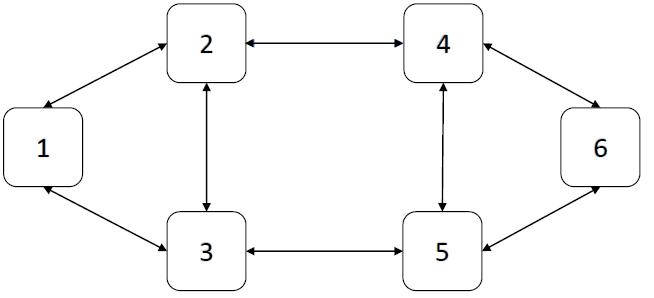
\includegraphics[width=\textwidth]{RedeTeste}
\caption{Physical Topology of the Reference Network.}
\end{figure}


The following table shows the values of the variables associated with this network.
\begin{table}[h!]
\centering
\begin{tabular}{|| c | c | c||}
 \hline
 Constant & Description & Value \\
 \hline\hline
 N & Number of Nodes & 6 \\
 L & Number of Bidirectional Links & 8 \\
 <$\delta$> & Node out-degree & 2,667 \\
 <len> & Mean Link Length (km) & 500 \\
 <h> & Mean Number of Hops,for Working Paths & 1,533 \\
 <h'> & Mean Number of Hops,for Backup Paths & 2,467 \\
 \hline
\end{tabular}
\caption{Table of reference network values}
\label{table:1}
\end{table}

As we can see from table \ref{table:1}, to do all the calculations necessary for this project, let us know the value of the traffic used. This value is defined depending on the scenario used, as we can see:
\begin{itemize}
  \item Low Traffic: \textbf{0.5 TBits/s}
  \item High Traffic: \textbf{5 TBits/s}
\end{itemize}

\subsubsection{Realistic Network}
The real network chosen for this work is the EON (European Optical Network).
The way the nodes are arranged geographically can be seen from the following figure.

\begin{figure}[h!]
\centering
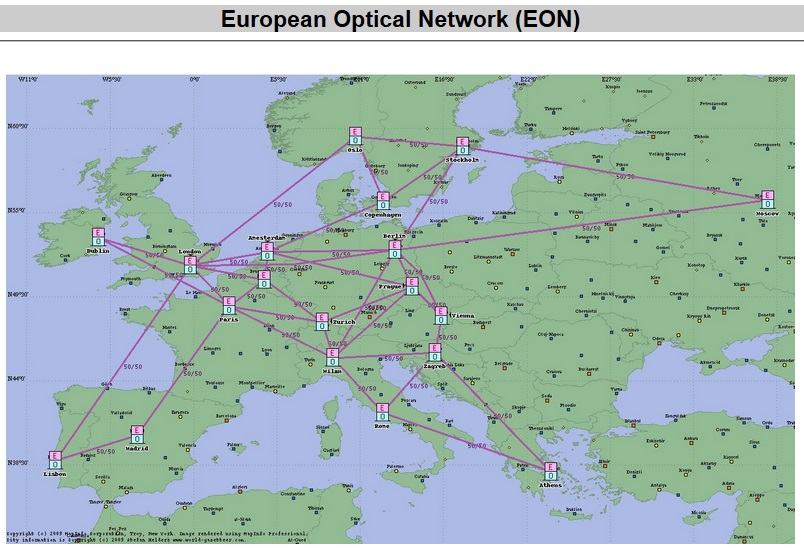
\includegraphics[width=\textwidth]{EON_Rede_Realista}
\caption{Physical Topology of the Realistic Network.}
\end{figure}

\begin{table}[h!]
The table \ref{table:2} shows the values of the variables associated with this network.\vspace{10pt}
\centering
\begin{tabular}{|| c | c | c||}
 \hline
 Constant & Description & Value \\
 \hline\hline
 N & Number of Nodes & 19 \\
 L & Number of Bidirectional Links & 37 \\
 <$\delta$> & Node out-degree & 3,89 \\
 <len> & Mean Link Length (km) & 753,76 \\
 <h> & Mean Number of Hops,for Working Paths & 2,3 \\
 <h'> & Mean Number of Hops,for Backup Paths & 3,2 \\
 \hline
\end{tabular}
\caption{Table of realistic network values}
\label{table:2}
\end{table}

Again, to make all the necessary calculations, only the value of the traffic used is missing. This value is set depending on the scenario used, as we can see:

\begin{itemize}
  \item Low Traffic: \textbf{2 TBits/s}
  \item High Traffic: \textbf{20 TBits/s}
\end{itemize}

\subsection{Dimensioning using ILP}

\subsubsection{ILP models}\label{ILP_models_OP}
The objective function of following ILP is a minimization of the sum of two variables: total number of flows crossing link (i; j) for all demand pairs (o; d) and total number of optical channels in each link (i; j).

\begin{equation}
minimize    \sum_{(i,j)} \sum_{(o,d)} f_{ij}^{od} + \sum_{(i,j)} W_{ij}
\label{ILPOpaque}
\end{equation}

$subject$ $to$
\begin{equation}
\sum_{j\textbackslash \{o\}} f_{ij}^{od} = 2  \qquad \qquad \qquad \qquad \qquad \qquad \qquad \qquad \qquad \qquad
\forall(o,d) : o < d, \forall i: i = o
\label{ILPOpaque1}
\end{equation}

\vspace{-5pt}
\begin{equation}
\sum_{j\textbackslash \{o\}} f_{ij}^{od} = \sum_{j\ \{d\}} f_{ji}^{od}   \qquad \qquad \qquad \qquad \qquad \qquad \qquad \qquad
\forall(o,d) : o < d, \forall i: i \neq o,d
\label{ILPOpaque2}
\end{equation}

\vspace{-5pt}
\begin{equation}
\sum_{j\textbackslash \{d\}} f_{ji}^{od} = 2  \qquad \qquad \qquad \qquad \qquad \qquad \qquad \qquad \qquad \qquad
\forall(o,d) : o < d, \forall i: i = d
\label{ILPOpaque3}
\end{equation}

\vspace{-5pt}
\begin{equation}
\sum_{(o,d):o<d} \left(f_{ij}^{od} + f_{ji}^{od}\right) + \sum_{c\in C} (B\left(c\right) D_{cod}\leq100 W_{ij} G_{ij} \qquad \qquad \qquad \qquad \qquad
\forall(i,j) : i < j
\label{ILPOpaque4}
\end{equation}

\vspace{-5pt}
\begin{equation}
W_{ij} \leq 80 \qquad  \qquad \qquad \qquad \qquad \qquad \qquad \qquad \qquad \qquad \qquad \qquad \qquad \forall(i,j) : i < j
\label{ILPOpaque5}
\end{equation}

\vspace{-5pt}
\begin{equation}
f_{ij}^{od} , f_{ji}^{od} \in \{0,2\}   \qquad \qquad \qquad \qquad \qquad \qquad \qquad \qquad \qquad
\forall(i,j) : i < j, \forall(o,d) : o < d
\label{ILPOpaque6}
\end{equation}

\vspace{-5pt}
\begin{equation}
W_{ij} \in \mathbb{N}  \qquad \qquad \qquad \qquad \qquad \qquad \qquad \qquad \qquad \qquad \qquad \qquad \qquad
\forall(i,j) : i < j\label{ILPOpaque7}
\end{equation}


The objective function, to be minimized, is the expression \ref{ILPOpaque}. The flow conservation constraints are \ref{ILPOpaque1}, \ref{ILPOpaque2} and \ref{ILPOpaque3}. First constraint ensures that, for all demand pairs (o,d), it routes two flows of traffic for all bidirectional links (i,j) when $j$ is not equal to the origin of the demand. Equation \ref{ILPOpaque3} is based on the same idea of \ref{ILPOpaque}, however applied in reverse direction. Assuming bidirectional traffic, so the number of flows in both directions of the link is the same \ref{ILPOpaque2}. The inequality \ref{ILPOpaque4} is considered grooming constraint, so it means the total client traffic flows can not be greater than the capacity of optical channels on all links. Another important constraint \ref{ILPOpaque5} is the capacity of the optical channels which must be less or equal to 100 Gb/s or 80 ODU0. The number of flows per demand can be zero if there are no traffic demands or two if considering working and protection traffic \ref{ILPOpaque6}. The last constraint is just needed to ensure the number optical of channels is a positive integer values greater than zero.


\subsubsection{ILP Results}

In this initial phase the results will be presented using ILP to calculate the CAPEX of the reference network.

The value of the CAPEX of the network will be calculated based on the costs of the equipment present in the figure below.
\begin{figure}[h!]
  \centering
  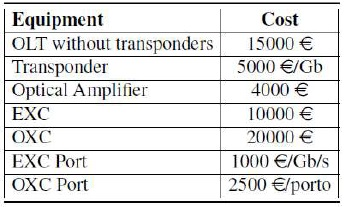
\includegraphics[scale=1]{TabValor}
  \caption{Table with costs}
  \label{TabCustOp}
\end{figure}

In addition to the equipment costs, we will also use the parameter "span", which in this case will have a value of 100.
Because this value is used to calculate the number of optical amplifiers required in the network using Equation \ref{amplifiers}.

\begin{equation}
N^R = \sum\limits_{l=1}^L\left(\left\lceil\frac{len_l}{span}\right\rceil-1\right)
\label{amplifiers}
\end{equation}

The other parameters of this equation are:
\begin{itemize}
\item{$N^R$			$\rightarrow$ Total number of regenerators/amplifiers}
\item{$len_l$		$\rightarrow$ Length of link l}
\item{$span$		$\rightarrow$ Distance between amplifiers}	
\end{itemize}	

To know the value of CAPEX it is necessary to know the value of the cost of the links and the cost of the nodes.

To calculate the cost of the nodes, the sum of the costs of the optical and electrical node is made. For this case the value of the optical cost is zero only needing to know the electric cost of the nodes that is given by equation \ref{electricalCostOpaque}.

\begin{equation}
C_{exc} = \left(\gamma_{e0}\times N\right) + \gamma_{e1} \times \left(T_1 + \left(2 \times w^0 \times \tau \right)\right)
\label{electricalCostOpaque}
\end{equation}

\begin{itemize}
\item{$C_{exc}$		$\rightarrow$	Electrical Ports Cost}
\item{$\gamma_{e0}$	$\rightarrow$	EXC cost in Euros}
\item{$N$			$\rightarrow$	Number of Nodes}
\item{$\gamma_{e1}$	$\rightarrow$	EXC port cost in Euros}
\item{$T_1$         $\rightarrow$   Total Unidirectional Traffic}
\item{$w^0$			$\rightarrow$	Total number of optical channels}
\item{$\tau$		$\rightarrow$	Traffic per port}
\end{itemize}

To calculate the cost of the Links we will use the equation \ref{linkCosts}.

\begin{equation}
C_L = \left(\gamma_0^{OLT} \times L\right) + \left(\gamma_1^{OLT} \times \tau \times W\right) + \left(N^R \times c^R\right)
\label{linkCosts}
\end{equation}	
	
\begin{itemize}
\item{$C_L$				$\rightarrow$	Links Cost}
\item{$\gamma_0^{OLT}$	$\rightarrow$	OLT cost in Euros}
\item{$L$				$\rightarrow$	Number of unidirectional Links}
\item{$\gamma_1^{OLT}$	$\rightarrow$	Transponder cost in Euros}
\item{$W$             $\rightarrow$	Total number of optical channels}
\item{$N^R$				$\rightarrow$	Total number of optical amplifiers}
\item{$c^R$				$\rightarrow$	Optical amplifiers cost in Euros}
\end{itemize}

To perform the calculations using the implementation of the models described in section \ref{ILP_models_OP} it is necessary to use a mathematical software tool. For this we will use MATLAB which is ideal for dealing with linear programming problems and can call the LPsolve through an external interface.

\pagebreak
Using the values calculated through MatLab as well as the values indicated in table \ref{table:1} or table \ref{table:2} (depending on the scenario used) and figure \ref{TabCustOp} we can finally calculate the CAPEX value using equations \ref{electricalCostOpaque} and \ref{linkCosts} for the various situations mentioned.\\

\textbf{Low Traffic scenario:}\\

$C_L$ = \textbf{24 336 000\euro}

$C_N$ = $C_{exc}$ = \textbf{5 860 000\euro}

$CAPEX$ = 24 336 000 + 5 860 000 = \textbf{30 196 000\euro}\\

\textbf{High Traffic scenario:}\\

$C_L$ = \textbf{191 336 000\euro}

$C_N$ = $C_{exc}$ = \textbf{48 260 000 \euro}

$CAPEX$ = 191 336 000 + 48 260 000 = \textbf{239 596 000 \euro}\\

\subsection{Dimensioning using Heuristics}

\subsubsection{Heuristics Models}

\subsubsection{Heuristics Results}

\subsection{Analysis and comparison of results}

\clearpage

\section{Transparent with 1+1 Protection}
In this case study we focus on the transparent case with 1 + 1 protection.
In this mode of transport, the information travels in a route defined through optical channels between origin and destination nodes always in the optical domain and, consequently, physical topology and logical topology are different.
An advantage of this mode of transport is the possibility of transporting express traffic.
An disadvantage is that the capacity utilization of the optical channels is worse than in the opaque mode of transport due to grooming only customer signs with the same endpoints.

\subsection{Physical Network Topology}
\begin{tcolorbox}	
\begin{tabular}{p{2.75cm} p{0.2cm} p{10.5cm}} 	
\textbf{Student Name}  &:& Tiago Esteves    (October 03, 2017 - )\\
\textbf{Goal}          &:& Implement the dimensioning of optical networks in the transparent transport mode.
\end{tabular}
\end{tcolorbox}
\vspace{-5pt}

\subsubsection{Reference Network}
In the figure below we ca see that our reference network consists of 6 nodes and 8 Bidirectional links.
The matrix of distances between the respective nodes and the ODU's matrices are the same as those reported in the opaque transport mode.

\begin{figure}[h!]
\centering
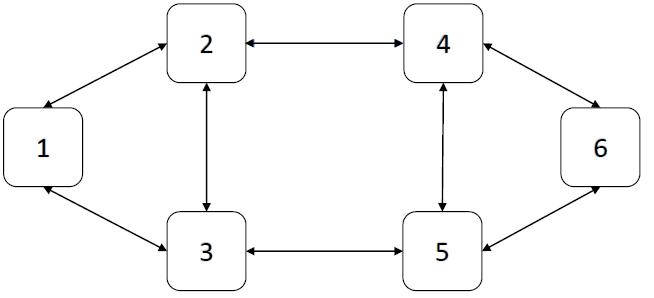
\includegraphics[width=\textwidth]{RedeTeste}
\caption{Physical Topology of the Reference Network.}
\end{figure}

The distance matrix is the same for the two scenarios but the ODU's matrices are not.
In this case only the matrices for the case of high traffic are elucidated, being that in the case of a low traffic it is only necessary to divide these matrices by the value 10.

\[
Dist=
  \begin{bmatrix}
    0 & 500 & 500 & 0 & 0 & 0 \\
    500 & 0 & 400 & 500 & 0 & 0 \\
    500 & 400 & 0 & 0 & 500 & 0 \\
    0 & 500 & 0 & 0 & 600 & 450 \\
    0 & 0 & 500 & 600 & 0 & 550 \\
    0 & 0 & 0 & 450 & 550 & 0
  \end{bmatrix}
\quad ODU0=
  \begin{bmatrix}
    0 & 50 & 10 & 30 & 10 & 30 \\
    50 & 0 & 0 & 10 & 50 & 0 \\
    10 & 0 & 0 & 10 & 40 & 10 \\
    30 & 10 & 10 & 0 & 10 & 0 \\
    10 & 50 & 40 & 10 & 0 & 30 \\
    30 & 0 & 10 & 10 & 30 & 0
  \end{bmatrix}
\]
\[
ODU1=
  \begin{bmatrix}
    0 & 20 & 40 & 20 & 0 & 50 \\
    20 & 0 & 0 & 30 & 10 & 10 \\
    40 & 0 & 0 & 10 & 10 & 0 \\
    30 & 30 & 10 & 0 & 10 & 30 \\
    0 & 10 & 10 & 10 & 0 & 10 \\
    50 & 10 & 0 & 30 & 10 & 0
  \end{bmatrix}
\quad ODU2=
  \begin{bmatrix}
    0 & 10 & 10 & 10 & 0 & 0 \\
    10 & 0 & 0 & 0 & 10 & 0 \\
    10 & 0 & 0 & 10 & 10 & 0 \\
    10 & 0 & 10 & 0 & 10 & 0 \\
    0 & 10 & 10 & 10 & 0 & 10 \\
    0 & 0 & 0 & 0 & 10 & 0
  \end{bmatrix}
\]
\[
ODU3=
  \begin{bmatrix}
    0 & 0 & 0 & 0 & 0 & 0 \\
    0 & 0 & 10 & 0 & 0 & 10 \\
    0 & 10 & 0 & 0 & 10 & 0 \\
    0 & 0 & 0 & 0 & 0 & 0 \\
    0 & 0 & 10 & 0 & 0 & 0 \\
    0 & 10 & 0 & 0 & 0 & 0
  \end{bmatrix}
\qquad ODU4=
  \begin{bmatrix}
    0 & 0 & 0 & 0 & 0 & 0 \\
    0 & 0 & 0 & 0 & 0 & 10 \\
    0 & 0 & 0 & 0 & 0 & 0 \\
    0 & 0 & 0 & 0 & 0 & 0 \\
    0 & 0 & 0 & 0 & 0 & 10 \\
    0 & 10 & 0 & 0 & 10 & 0
  \end{bmatrix}
\]

Through these ODU's we can calculate total network traffic for the low traffic scenario:\\
$T_1^0$ = 600x1.25 = 750 Gbits/s \qquad
$T_1^1$ = 500x2.5 = 1250 Gbits/s \qquad
$T_1^2$ = 160x10 = 1600 Gbits/s \\
$T_1^3$ = 60x40 = 2400 Gbits/s \quad
$T_1^4$ = 40x100 = 4000 Gbits/s \\
$T_{1total}$ = 750 + 1250 + 1600 + 2400 + 4000 = 10000 Gbits/s \qquad
$T_{total}$ = 10000/2 = 5 Tbits/s\\

We can thus conclude that the total traffic for the two scenarios is as follows:
\begin{itemize}
  \item Low Traffic: \textbf{0.5 TBits/s}
  \item High Traffic: \textbf{5 TBits/s}
\end{itemize}

Finally for this project has to take into consideration the table \ref{table:3} because in it we can see the values of the variables associated with this network.
\begin{table}[h!]
\centering
\begin{tabular}{|| c | c | c||}
 \hline
 Constant & Description & Value \\
 \hline\hline
 N & Number of nodes & 6 \\
 L & Number of bidirectional links & 8 \\
 <$\delta$> & Node out-degree & 2.667 \\
 <len> & Mean link length (km) & 500 \\
 <h> & Mean number of hops for working paths & 1.533 \\
 <h'> & Mean number of hops for backup paths & 2.467 \\
 \hline
\end{tabular}
\caption{Table of reference network values}
\label{table:3}
\end{table}


\subsubsection{Realistic Network}
The real network chosen for this work is the EON (European Optical Network).
The way the nodes are arranged geographically can be seen from the following figure and the matrix of distances created in the next page is constructed based on real distances.
In this case just ODU's matrices are created to be able to determine the total traffic used in each scenario.

\begin{figure}[h!]
\centering
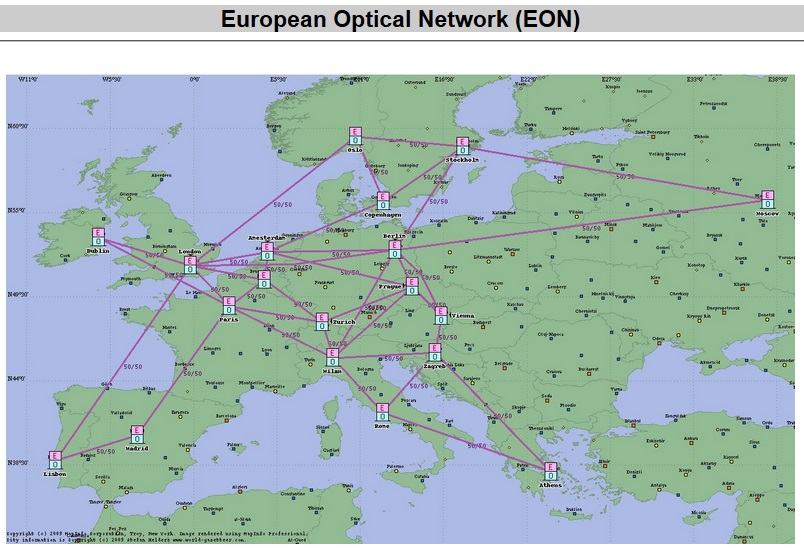
\includegraphics[width=\textwidth]{EON_Rede_Realista}
\caption{Physical Topology of the Realistic Network.}
\end{figure}

The table \ref{table:4} shows the values of the variables associated with this network.
\begin{table}[h!]
\centering
\begin{tabular}{|| c | c | c||}
 \hline
 Constant & Description & Value \\
 \hline\hline
 N & Number of nodes & 19 \\
 L & Number of bidirectional links & 37 \\
 <$\delta$> & Node out-degree & 3.89 \\
 <len> & Mean link length (km) & 753.76 \\
 <h> & Mean number of hops for working paths & 2.3 \\
 <h'> & Mean number of hops for backup paths & 3.2 \\
 \hline
\end{tabular}
\caption{Table of realistic network values}
\label{table:4}
\end{table}

Again, through the ODU's we can calculate the total traffic for both scenarios being them:
\begin{itemize}
  \item Low Traffic: \textbf{2 TBits/s}
  \item High Traffic: \textbf{20 TBits/s}
\end{itemize}


\[
  \text{Dist} = \kbordermatrix{
    & Oslo & Stockholm & Moscow & Copenhagen & Berlin & Prague & Vienna & Zagreb & Athens & Rome & Milan & Zurich & Brussels & Amesterdan & London & Dublin & Paris & Madrid & Lisbon \\
    Oslo & 0 & 500 & 500 & 0 & 0 & 0 & 0 & 500 & 500 & 0 & 0 & 500 & 500 & 0 & 0 & 0 & 0 & 500 & 500 \\
    Stockholm & 0 & 500 & 500 & 0 & 0 & 0 & 0 & 500 & 500 & 0 & 0 & 500 & 500 & 0 & 0 & 0 & 0 & 500 & 500 \\
    Moscow & 0 & 500 & 500 & 0 & 0 & 0 & 0 & 500 & 500 & 0 & 0 & 500 & 500 & 0 & 0 & 0 & 0 & 500 & 500 \\
    Copenhagen & 0 & 500 & 500 & 0 & 0 & 0 & 0 & 500 & 500 & 0 & 0 & 500 & 500 & 0 & 0 & 0 & 0 & 500 & 500 \\
    Berlin & 0 & 500 & 500 & 0 & 0 & 0 & 0 & 500 & 500 & 0 & 0 & 500 & 500 & 0 & 0 & 0 & 0 & 500 & 500 \\
    Prague & 0 & 500 & 500 & 0 & 0 & 0 & 0 & 500 & 500 & 0 & 0 & 500 & 500 & 0 & 0 & 0 & 0 & 500 & 500 \\
    Vienna & 0 & 500 & 500 & 0 & 0 & 0 & 0 & 500 & 500 & 0 & 0 & 500 & 500 & 0 & 0 & 0 & 0 & 500 & 500 \\
    Zagreb & 0 & 500 & 500 & 0 & 0 & 0 & 0 & 500 & 500 & 0 & 0 & 500 & 500 & 0 & 0 & 0 & 0 & 500 & 500 \\
    Athens & 0 & 500 & 500 & 0 & 0 & 0 & 0 & 500 & 500 & 0 & 0 & 500 & 500 & 0 & 0 & 0 & 0 & 500 & 500 \\
    Rome & 0 & 500 & 500 & 0 & 0 & 0 & 0 & 500 & 500 & 0 & 0 & 500 & 500 & 0 & 0 & 0 & 0 & 500 & 500 \\
    Milan & 0 & 500 & 500 & 0 & 0 & 0 & 0 & 500 & 500 & 0 & 0 & 500 & 500 & 0 & 0 & 0 & 0 & 500 & 500 \\
    Zurich & 0 & 500 & 500 & 0 & 0 & 0 & 0 & 500 & 500 & 0 & 0 & 500 & 500 & 0 & 0 & 0 & 0 & 500 & 500 \\
    Brussels & 0 & 500 & 500 & 0 & 0 & 0 & 0 & 500 & 500 & 0 & 0 & 500 & 500 & 0 & 0 & 0 & 0 & 500 & 500 \\
    Amesterdan & 0 & 500 & 500 & 0 & 0 & 0 & 0 & 500 & 500 & 0 & 0 & 500 & 500 & 0 & 0 & 0 & 0 & 500 & 500 \\
    London & 0 & 500 & 500 & 0 & 0 & 0 & 0 & 500 & 500 & 0 & 0 & 500 & 500 & 0 & 0 & 0 & 0 & 500 & 500 \\
    Dublin & 0 & 500 & 500 & 0 & 0 & 0 & 0 & 500 & 500 & 0 & 0 & 500 & 500 & 0 & 0 & 0 & 0 & 500 & 500 \\
    Paris & 0 & 500 & 500 & 0 & 0 & 0 & 0 & 500 & 500 & 0 & 0 & 500 & 500 & 0 & 0 & 0 & 0 & 500 & 500\\
    Madrid & 0 & 500 & 500 & 0 & 0 & 0 & 0 & 500 & 500 & 0 & 0 & 500 & 500 & 0 & 0 & 0 & 0 & 500 & 500 \\
    Lisbon & 0 & 500 & 500 & 0 & 0 & 0 & 0 & 500 & 500 & 0 & 0 & 500 & 500 & 0 & 0 & 0 & 0 & 500 & 444
  }
\]


\newpage
\subsection{Dimensioning using ILP}
\begin{tcolorbox}	
\begin{tabular}{p{2.75cm} p{0.2cm} p{10.5cm}} 	
\textbf{Student Name}  &:& Tiago Esteves    (October 03, 2017 - )\\
\textbf{Goal}          &:& Implement the dimensioning of optical networks in the transparent transport mode.
\end{tabular}
\end{tcolorbox}

\subsubsection{ILP Models} \label{ILP_models_Transp}

Again, for a better understanding of the functions and variables used in the ILP, a table \ref{description_transp} will be created with all the variables and their description. \\

\begin{table}[h!]
\centering
\begin{tabular}{ |p{1cm}||p{13cm}|}
 \hline
 \multicolumn{2}{|c|}{Description of notation used in the objective function} \\
 \hline
 \hline
 $i$ & index for start node of a physical link \\
 $j$ & index for end node of a physical link \\
 $o$ & index for node that is origin of a demand \\
 $d$ & index for node that is destination of a demand \\
 $($ i,j $)$ & physical link between the nodes $i$ and $j$ \\
 $($ o,d $)$ & demand between the nodes $o$ and $d$ \\
 $f_{ij}^{od}$ & Number of 100 Gbit/s optical channels (number of flows) between the link $i$ and $j$ for all demand pairs between $o$ and $d$ \\
 $W_{od}$ & number of optical channels between the nodes $o$ and $d$\\
 G & Network topology in form of adjacency matrix \\
 \hline
\end{tabular}
\caption{Table with description of variables}
\label{description_transp}
\end{table}


The optimization model suggested for transparent transport mode with dedicated path protection intends to minimize the total number of flows crossing link (i, j) for all demand pairs (o, d). The mathematical model described below also minimizes the total number of optical channels between each demand end nodes $W_{od}$, instead of minimizing the number of optical link-by-link channels as in the previous model.

\vspace{10pt}
\begin{equation}
minimize    \sum_{(i,j)} \sum_{(o,d)} f_{ij}^{od} + \sum_{(o,d)} W_{od}
\label{ILPTransp}
\end{equation}

$subject$ $to$
\begin{equation}
\sum_{j\textbackslash \{o\}} f_{ij}^{od} = 2  \qquad \qquad \qquad \qquad \qquad \qquad \qquad \qquad \qquad \qquad
\forall(o,d) : o < d, \forall i: i = o
\label{ILPTransp1}
\end{equation}

\begin{equation}
\sum_{j\textbackslash \{o\}} f_{ij}^{od} = \sum_{j\textbackslash \{d\}} f_{ji}^{od}   \qquad \qquad \qquad \qquad \qquad \qquad \qquad \qquad
\forall(o,d) : o < d, \forall i: i \neq o,d
\label{ILPTransp2}
\end{equation}

\begin{equation}
\sum_{j\textbackslash \{d\}} f_{ji}^{od} = 2  \qquad \qquad \qquad \qquad \qquad \qquad \qquad \qquad \qquad \qquad
\forall(o,d) : o < d, \forall i: i = d
\label{ILPTransp3}
\end{equation}

\begin{equation}
\sum_{(o,d):o<d} \left(f_{ij}^{od} + f_{ji}^{od}\right) W_{od} \leq 80 G_{ij} \qquad \qquad \qquad \qquad \qquad \qquad \qquad \qquad
\forall(i,j) : i < j
\label{ILPTransp4}
\end{equation}

\begin{equation}
f_{ij}^{od} , f_{ji}^{od} \in \{0,2\}   \qquad \qquad \qquad \qquad \qquad \qquad \qquad \qquad \qquad
\forall(i,j) : i < j, \forall(o,d) : o < d
\label{ILPTransp5}
\end{equation}

\begin{equation}
W_{od} \in \mathbb{N}  \qquad \qquad \qquad \qquad \qquad \qquad \qquad \qquad \qquad \qquad \qquad \qquad \qquad
\forall(o,d) : o < d
\label{ILPTransp6}
\end{equation}


The objective function, to be minimized, is the expression \ref{ILPTransp}. The flow conservation is performed by equations \ref{ILPTransp1}, \ref{ILPTransp2} and \ref{ILPTransp3} and share the same mathematical description of opaque model. The inequality \ref{ILPTransp4} answers capacity constraint problem. Then, total flows times the traffic of the demands must be less or equal to the capacity of network links. The grooming of this model can be done before routing since the traffic is aggregated just for demands between the same nodes, thus not depending on the routes. Last two constraints define the total number of flows must be zero if there is no demand, or two for a demand with traffic protection, and the number of optical channels must be a counting number.

\subsubsection{ILP Results}

In this initial phase the results will be presented using ILP to calculate the CAPEX of the reference network and the realistic network.
The value of the CAPEX of the network will be calculated based on the costs of the equipment present in the table below.

\begin{table}[h!]
\centering
\begin{tabular}{|| c | c||}
 \hline
 Equipment & Cost \\
 \hline\hline
 OLT without transponders & 15000 \euro \\
 Transponder & 5000 \euro/Gb \\
 Optical Amplifier & 4000 \euro \\
 EXC & 10000 \euro \\
 OXC & 20000 \euro \\
 EXC Port & 1000 \euro /Gb/s\\
 OXC Port & 2500 \euro /porto \\
 \hline
\end{tabular}
\caption{Table with costs}
\label{table_cost2}
\end{table}

In addition to the equipment costs we will also use the parameter "span", which in this case will have a value of 100, because this value is used to calculate the number of optical amplifiers required in the network using Equation \ref{amplifiersTransp}.

\begin{equation}
N^R = \sum\limits_{l=1}^L\left(\left\lceil\frac{len_l}{span}\right\rceil-1\right)
\label{amplifiersTransp}
\end{equation} \\

To know the value of CAPEX it is necessary to know the value of the cost of the links and the cost of the nodes.

To calculate the cost of the nodes, the sum of the costs of the optical and electrical node is made. For this case the optical cost is given by equation \ref{opticalCost} and the electrical cost by the equation \ref{electricalCostTransp}.


\begin{equation}
C_{oxc} = \left(\gamma_{o0} \times N \right) + \gamma_{o1} \times  \left(P_{LINE} + P_{ADD}\right)
\label{opticalCost}
\end{equation}	
	
\begin{itemize}
\item{$C_{oxc}$		$\rightarrow$	Optical Ports Cost}
\item{$\gamma_{o0}$	$\rightarrow$	OXC cost in Euros}
\item{$\gamma_{o1}$	$\rightarrow$	OXC port cost in Euros}
\item{$P_{TRIB}	$	$\rightarrow$	Number of tributary ports}
\item{$P_{ADD} $	$\rightarrow$	Number of adding ports}
\end{itemize}

\begin{equation}
C_{exc} = \left(\gamma_{e0}\times N\right) + \gamma_{e1} \times \left(2 \times T_1 \right)		\label{electricalCostTransp}
\end{equation}

\vspace{10pt}

To calculate the cost of the Links we will use the equation \ref{linkCostsTransp}.

\begin{equation}
C_L = \left(2 \times \gamma_0^{OLT} \times L\right) + \left(2 \times \gamma_1^{OLT} \times \tau \times W\right) + \left(N^R \times c^R\right)
\label{linkCostsTransp}
\end{equation} \\
	
\vspace{11pt}
To perform the calculations using the implementation of the models described in section \ref{ILP_models_OP} it is necessary to use a mathematical software tool. For this we will use MATLAB which is ideal for dealing with linear programming problems and can call the LPsolve through an external interface. \\

\textbf{Scenario 1: Test Network Low Traffic} \label{Scenario1_transp} \\
In this scenario we used the table \ref{table:3}. In the table \ref{result_ILP1_T} we can see the values calculated through MatLab and using the values indicated in table \ref{table_cost2} we can finally calculate the CAPEX value. \\
\newpage
\begin{table}[h!]
\centering
\begin{tabular}{|| c | c||}
 \hline
 Number of optical channels & Value \\
 \hline\hline
 in the link (1,2) & 2 \\
 in the link (1,3) & 2 \\
 in the link (2,3) & 4 \\
 in the link (2,4) & 3 \\
 in the link (3,5) & 3 \\
 in the link (4,5) & 3 \\
 in the link (4,6) & 3 \\
 in the link (5,6) & 3 \\
 \hline
\end{tabular}
\caption{Table with results}
\label{result_ILP1_T}
\end{table}

Using equation \ref{linkCostsTransp} : \\
$C_L$ = $($2 * 15 000 * 8$)$ + $($2 * 5 000 * 100 * $)$ + $($24 * 4 000$)$ \\
$C_L$ = \textbf{ \euro} \\

Using equation \ref{electricalCostTransp} : \\
$C_{exc}$ = $($6 * 10 000$)$ + 1 000 * $($2 * 1 000$)$ \\
$C_{exc}$ = \textbf{2 060 000\euro} \\

Using equation \ref{opticalCost} : \\
$C_{oxc}$ = $($6 * 10 000$)$ + 1 000 * $($ + $)$ \\
$C_{oxc}$ = \textbf{ \euro} \\
$C_N$ = $C_{oxc}$ + $C_{exc}$ = \textbf{ \euro} \\

$CAPEX$ =  +  = \textbf{ \euro}\\

\textbf{Scenario 2: Test Network High Traffic} \label{Scenario2_transp} \\
In this scenario we used again the table \ref{table:3} In the table \ref{result_ILP2_T} we can see the values calculated through MatLab and using the values indicated in table \ref{table_cost2} we can finally calculate the CAPEX value.

\begin{table}[h!]
\centering
\begin{tabular}{|| c | c||}
 \hline
 Number of optical channels & Value \\
 \hline\hline
 in the link (1,2) & 2 \\
 in the link (1,3) & 2 \\
 in the link (2,3) & 4 \\
 in the link (2,4) & 3 \\
 in the link (3,5) & 3 \\
 in the link (4,5) & 3 \\
 in the link (4,6) & 3 \\
 in the link (5,6) & 3 \\
 \hline
\end{tabular}
\caption{Table with results}
\label{result_ILP2_T}
\end{table}


Using equation \ref{linkCostsTransp} : \\
$C_L$ = $($2 * 15 000 * 8$)$ + $($2 * 5 000 * 100 * $)$ + $($24 * 4 000$)$ \\
$C_L$ = \textbf{ \euro} \\

Using equation \ref{electricalCostTransp} : \\
$C_{exc}$ = $($6 * 10 000$)$ + 1 000 * $($2 * 2 000$)$ \\
$C_{exc}$ = \textbf{4 060 000 \euro} \\

Using equation \ref{opticalCost} : \\
$C_{oxc}$ = $($6 * 10 000$)$ + 1 000 * $($ + $)$ \\
$C_{oxc}$ = \textbf{ \euro} \\
$C_N$ = $C_{oxc}$ + $C_{exc}$ = \textbf{ \euro} \\

$CAPEX$ =  +  = \textbf{ \euro}\\


\vspace{11pt}
\textbf{Scenario 3: Realistic Network Low Traffic} \label{Scenario3_transp} \\
In this scenario we used the table \ref{table:4} In the table \ref{result_ILP3_T} we can see the values calculated through MatLab and using the values indicated in table \ref{table_cost2} we can finally calculate the CAPEX value. \\

\begin{table}[h!]
\centering
\begin{tabular}{|| c | c||}
 \hline
 Number of optical channels & Value \\
 \hline\hline
 in the link (1,2) & 2 \\
 in the link (1,3) & 2 \\
 in the link (2,3) & 4 \\
 in the link (2,4) & 3 \\
 in the link (3,5) & 3 \\
 in the link (4,5) & 3 \\
 in the link (4,6) & 3 \\
 in the link (5,6) & 3 \\
 \hline
\end{tabular}
\caption{Table with results}
\label{result_ILP3_T}
\end{table}

Using equation \ref{linkCostsTransp} : \\
$C_L$ = $($2 * 15 000 * 37$)$ + $($2 * 5 000 * 100 * $)$ + $($24 * 4 000$)$ \\
$C_L$ = \textbf{ \euro} \\

Using equation \ref{electricalCostTransp} : \\
$C_{exc}$ = $($19 * 10 000$)$ + 1 000 * $($2 * 4 000$)$ \\
$C_{exc}$ = \textbf{8 190 000\euro} \\

Using equation \ref{opticalCost} : \\
$C_{oxc}$ = $($19 * 10 000$)$ + 1 000 * $($ + $)$ \\
$C_{oxc}$ = \textbf{ \euro} \\
$C_N$ = $C_{oxc}$ + $C_{exc}$ = \textbf{ \euro} \\

$CAPEX$ =  +  = \textbf{ \euro}\\


\vspace{11pt}
\textbf{Scenario 4: Realistic Network High Traffic} \label{Scenario4_transp} \\
In this scenario we used again the table \ref{table:4} In the table \ref{result_ILP4_T} we can see the values calculated through MatLab and using the values indicated in table \ref{table_cost2} we can finally calculate the CAPEX value. \\

\begin{table}[h!]
\centering
\begin{tabular}{|| c | c||}
 \hline
 Number of optical channels & Value \\
 \hline\hline
 in the link (1,2) & 2 \\
 in the link (1,3) & 2 \\
 in the link (2,3) & 4 \\
 in the link (2,4) & 3 \\
 in the link (3,5) & 3 \\
 in the link (4,5) & 3 \\
 in the link (4,6) & 3 \\
 in the link (5,6) & 3 \\
 \hline
\end{tabular}
\caption{Table with results}
\label{result_ILP4_T}
\end{table}

Using equation \ref{linkCostsTransp} : \\
$C_L$ = $($2 * 15 000 * 37$)$ + $($2 * 5 000 * 100 * $)$ + $($24 * 4 000$)$ \\
$C_L$ = \textbf{ \euro} \\

Using equation \ref{electricalCostTransp} : \\
$C_{exc}$ = $($19 * 10 000$)$ + 1 000 * $($2 * 40 000$)$ \\
$C_{exc}$ = \textbf{80 190 000\euro} \\

Using equation \ref{opticalCost} : \\
$C_{oxc}$ = $($19 * 10 000$)$ + 1 000 * $($ + $)$ \\
$C_{oxc}$ = \textbf{ \euro} \\
$C_N$ = $C_{oxc}$ + $C_{exc}$ = \textbf{ \euro} \\

$CAPEX$ =  +  = \textbf{ \euro}\\

\newpage

\subsection{Dimensioning using Heuristics}

\subsubsection{Heuristics Models}

\subsubsection{Heuristics Results}

\subsection{Comparative Analysis} 
\clearpage

\begin{tcolorbox}	
\begin{tabular}{p{2.75cm} p{0.2cm} p{10.5cm}} 	
\textbf{Student Name}  &:& Tiago Esteves\\
\textbf{Starting Date} &:& October 03, 2017\\
\textbf{Goal}          &:& Implement the dimensioning of optical networks in the translucent transport mode.
\end{tabular}
\end{tcolorbox}

\section{Translucent with 1+1 Protection}
In this case study we focus on the translucent case with 1 + 1 protection.


\subsection{Physical Network Topology}

\subsubsection{Reference Network}
As we can see in the figure, our reference network consists of 6 nodes and 8 Bidirectional links.
The average length of the links was chosen so that the following calculations are more simplistic.

\begin{figure}[h!]
\centering
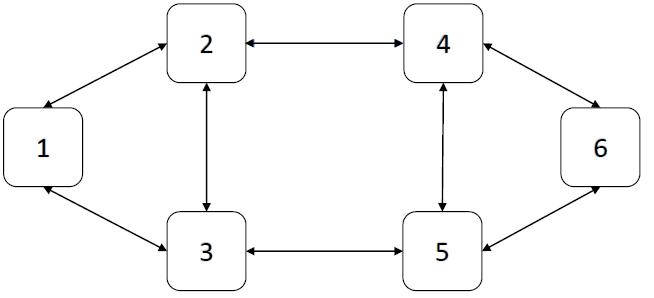
\includegraphics[width=\textwidth]{RedeTeste}
\caption{Physical Topology of the Reference Network.}
\end{figure}

The following table shows the values of the variables associated with this network.
\begin{table}[h!]
\centering
\begin{tabular}{|| c | c | c||}
 \hline
 Constant & Description & Value \\
 \hline\hline
 N & Number of Nodes & 6 \\
 L & Number of Bidirectional Links & 8 \\
 <$\delta$> & Node out-degree & 2,667 \\
 <len> & Mean Link Length (km) & 500 \\
 <h> & Mean Number of Hops,for Working Paths & 1,533 \\
 <h'> & Mean Number of Hops,for Backup Paths & 2,467 \\
 \hline
\end{tabular}
\caption{Table of reference network values}
\label{table:5}
\end{table}

As we can see from table \ref{table:5}, to do all the calculations necessary for this project, let us know the value of the traffic used. This value is defined depending on the scenario used, as we can see:
\begin{itemize}
  \item Low Traffic: \textbf{0.5 TBits/s}
  \item High Traffic: \textbf{5 TBits/s}
\end{itemize}

\subsubsection{Realistic Network}
The real network chosen for this work is the EON (European Optical Network). \\
The way the nodes are arranged geographically can be seen from the following figure.

\begin{figure}[h!]
\centering
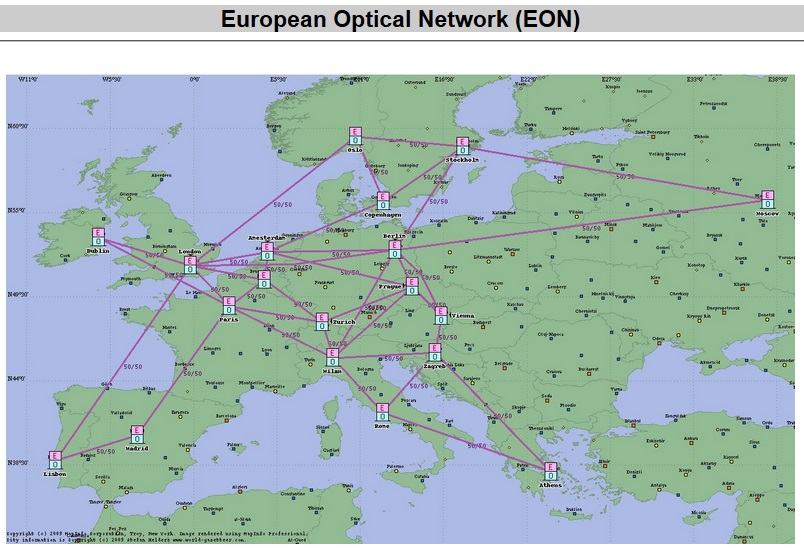
\includegraphics[width=\textwidth]{EON_Rede_Realista}
\caption{Physical Topology of the Realistic Network.}
\end{figure}


Again, to make all the necessary calculations, only the value of the traffic used is missing. This value is set depending on the scenario used, as we can see:

\begin{itemize}
  \item Low Traffic: \textbf{2 TBits/s}
  \item High Traffic: \textbf{20 TBits/s}
\end{itemize}

\begin{table}[h!]
The table \ref{table:6} shows the values of the variables associated with this network.\vspace{10pt}
\centering
\begin{tabular}{|| c | c | c||}
 \hline
 Constant & Description & Value \\
 \hline\hline
 N & Number of Nodes & 19 \\
 L & Number of Bidirectional Links & 37 \\
 <$\delta$> & Node out-degree & 3,89 \\
 <len> & Mean Link Length (km) & 753,76 \\
 <h> & Mean Number of Hops,for Working Paths & 2,3 \\
 <h'> & Mean Number of Hops,for Backup Paths & 3,2 \\
 \hline
\end{tabular}
\caption{Table of realistic network values}
\label{table:6}
\end{table}

\newpage
\subsection{Dimensioning using ILP}

\subsubsection{ILP models} \label{ILP_models_Transluc}

Again, for a better understanding of the functions and variables used in the ILP, a table \ref{description_transluc} will be created with all the variables and their description. \\

\begin{table}[h!]
\centering
\begin{tabular}{|| c | c||}
 \hline
 Variables & Description \\
 \hline\hline
 $($ i,j $)$ & Origin node, i and destination node, j of a Link \\
 $($ o,d $)$ & Origin node, o and destination node, d of a Demand \\
 c & Client traffic Type $($ 1 to 5 $)$ \\
 L &  \\
 y &  \\
 W & Number of optical channels \\
 B & Client signals granularities $($1.25, 2.5, 10, 40, 100$)$ \\
 D & Client traffic demands \\
 G & Network topology in form of Adjacency matrix \\
 BD & \\
 \hline
\end{tabular}
\caption{Table with description of variables}
\label{description_transluc}
\end{table}

\vspace{20pt}

\begin{equation}
minimize \qquad \qquad \qquad \qquad \qquad  \sum_{(o,d,b)} W_{od}
\label{ILPTransluc}
\end{equation}

$subject$ $to$

\begin{equation}
\sum_{j \neq i} L_{ij}^{od} = D_{odc}
\qquad \qquad \qquad \qquad \qquad \qquad \qquad \qquad \qquad
\forall o,c,d : o < d
\label{ILPTransluc1}
\end{equation}

\begin{equation}
\sum_{j \neq i \ j \neq o} L_{ij}^{od} = \sum_{j \neq i \ j \neq o} L_{ji}^{od}
\qquad \qquad \qquad \qquad \qquad \qquad
\forall s,d,p,o : s < d : p \neq s : p \neq d
\label{ILPTransluc2}
\end{equation}

\begin{equation}
\sum_{i \neq j} L_{ji}^{od} = D_{odc}
\qquad \qquad \qquad \qquad \qquad \qquad \qquad \qquad
\forall o,d,c : o < d
\label{ILPTransluc3}
\end{equation}

\begin{equation}
\sum_{(o,d,c): o<d} (B(c) \times L_{ij}^{od}) \leq  \sum_{b} BD_b \times W_{ijb}
\qquad \qquad \qquad \qquad \qquad
\forall i,j
\label{ILPTransluc4}
\end{equation}

\begin{equation}
L_{ij}^{od} \geq 0;
\qquad \qquad \qquad \qquad \qquad \qquad \qquad \qquad \qquad \qquad
\forall o,d,i,j : o < d
\label{ILPTransluc5}
\end{equation}

\begin{equation}
\sum_{i \neq j} y_{ij}^{od} = W_{od}
\qquad \qquad \qquad \qquad \qquad \qquad \qquad \qquad \qquad \qquad \qquad
\forall i,j,b
\label{ILPTransluc6}
\end{equation}

\begin{equation}
\sum_{j\neq i \ j\neq o} y_{ij}^{od} = \sum_{j \neq i \ j \neq d} y_{ji}^{od}
\qquad \qquad \qquad \qquad \qquad \qquad \qquad
\forall o,d,i,b : i \neq d : i \neq o
\label{ILPTransluc7}
\end{equation}

\begin{equation}
\sum_{j \neq i} y_{ji}^{od} = W_{od}
\qquad \qquad \qquad \qquad \qquad \qquad \qquad \qquad \qquad \qquad \qquad
\forall o,d,b
\label{ILPTransluc8}
\end{equation}

\begin{equation}
\sum_{(o,d,b)} \left( y_{ij}^{od} + y_{ji}^{od}\right) \leq 80 G_{ij}
\qquad \qquad \qquad \qquad \qquad \qquad \qquad
\forall i,j : i < j
\label{ILPTransluc9}
\end{equation}

\begin{equation}
y_{ij}^{od} \geq 0
\qquad \qquad \qquad \qquad \qquad \qquad \qquad \qquad \qquad \qquad \qquad \qquad
\forall o,d,i,j,b
\label{ILPTransluc10}
\end{equation}	


\subsubsection{ILP Results}

In this initial phase the results will be presented using ILP to calculate the CAPEX of the reference network.

The value of the CAPEX of the network will be calculated based on the costs of the equipment present in the table below.
\begin{table}[h!]
\centering
\begin{tabular}{|| c | c||}
 \hline
 Equipment & Cost \\
 \hline\hline
 OLT without transponders & 15000 \euro \\
 Transponder & 5000 \euro/Gb \\
 Optical Amplifier & 4000 \euro \\
 EXC & 10000 \euro \\
 OXC & 20000 \euro \\
 EXC Port & 1000 \euro /Gb/s\\
 OXC Port & 2500 \euro /porto \\
 \hline
\end{tabular}
\caption{Table with costs}
\label{table_cost3}
\end{table}

In addition to the equipment costs, we will also use the parameter "span", which in this case will have a value of 100.
Because this value is used to calculate the number of optical amplifiers required in the network using Equation \ref{amplifiersTranslu}.

\begin{equation}
N^R = \sum\limits_{l=1}^L\left(\left\lceil\frac{len_l}{span}\right\rceil-1\right)
\label{amplifiersTranslu}
\end{equation} \\

To know the value of CAPEX it is necessary to know the value of the cost of the links and the cost of the nodes.

To calculate the cost of the nodes, the sum of the costs of the optical and electrical node is made. %For this case the optical cost is given by equation \ref{opticalCost} and the electrical cost by the equation \ref{electricalCostTransp}.

%\begin{equation}
%C_{oxc} = \left(\gamma_{o0} \times N \right) + \gamma_{o1} \times  \left(P_{LINE} + P_{ADD}\right)
%\label{opticalCost}
%\end{equation}	
	
%\begin{itemize}
%\item{$C_{oxc}$		$\rightarrow$	Optical Ports Cost}
%\item{$\gamma_{o0}$	$\rightarrow$	OXC cost in Euros}
%\item{$\gamma_{o1}$	$\rightarrow$	OXC port cost in Euros}
%\item{$P_{TRIB}	$	$\rightarrow$	Number of tributary ports}
%\item{$P_{ADD} $	$\rightarrow$	Number of adding ports}
%\end{itemize}

%\begin{equation}
%C_{exc} = \left(\gamma_{e0}\times N\right) + \gamma_{e1} \times \left(2 \times T_1 \right)		\label{electricalCostTransp}
%\end{equation} \\


To calculate the cost of the Links we will use the equation .

%\begin{equation}
%C_L = \left(\gamma_0^{OLT} \times L\right) + \left(\gamma_1^{OLT} \times \tau \times W\right) + \left(N^R \times %c^R\right)
%\label{linkCostsTransp}
%\end{equation} \\
	

Finally we will calculate the CAPEX values for the various situations mentioned.\\

\textbf{Low Traffic scenario:}\\

$C_L$ = \textbf{\euro}

$C_N$ = \textbf{\euro}

$CAPEX$ = \textbf{\euro}\\

\textbf{High Traffic scenario:}\\

$C_L$ = \textbf{\euro}

$C_N$ = \textbf{ \euro}

$CAPEX$ =  \textbf{ \euro}\\

\subsection{Dimensioning using Analytical solution}

\subsubsection{Analytical Models}

\subsubsection{Analytical Results}

\newpage

\subsection{Dimensioning using Heuristics}

\subsubsection{Heuristics Models}

\subsubsection{Heuristics Results}

\subsection{Analysis and comparison of results}



% ------------------------------------------------------------------------
\chapter{Appendices}

\clearpage

\graphicspath{{./figures/}}
\section{Net2Plan guide}
This first section will describe how to install Net2Plan and some of the solvers usable by it as well as the main program preferences available.


    \subsection*{Net2Plan download and installation}
    \vspace{0.5cm}
	Before downloading Net2Plan, the first step is verifying if the computer has the necessary Java Runtime Environment, it is recommended the latest release (Version 8). This can be download from the java website at \url{https://java.com/en/download/}. The Java Runtime Environment is necessary as Net2Plan was coded in Java.
		
    Having installed the Java Environment it is now possible to install Net2Plan. The download is available on its website at \url{http://net2plan.com/download.php}. The files just need to be extracted and the program can be run without an installation by just double clicking on the file "Net2Plan.jar". The latest Net2Plan version available at the time this report was revised is 0.4.2 from July 22nd, 2016

    \begin{figure}[h!]
       	\centering
       	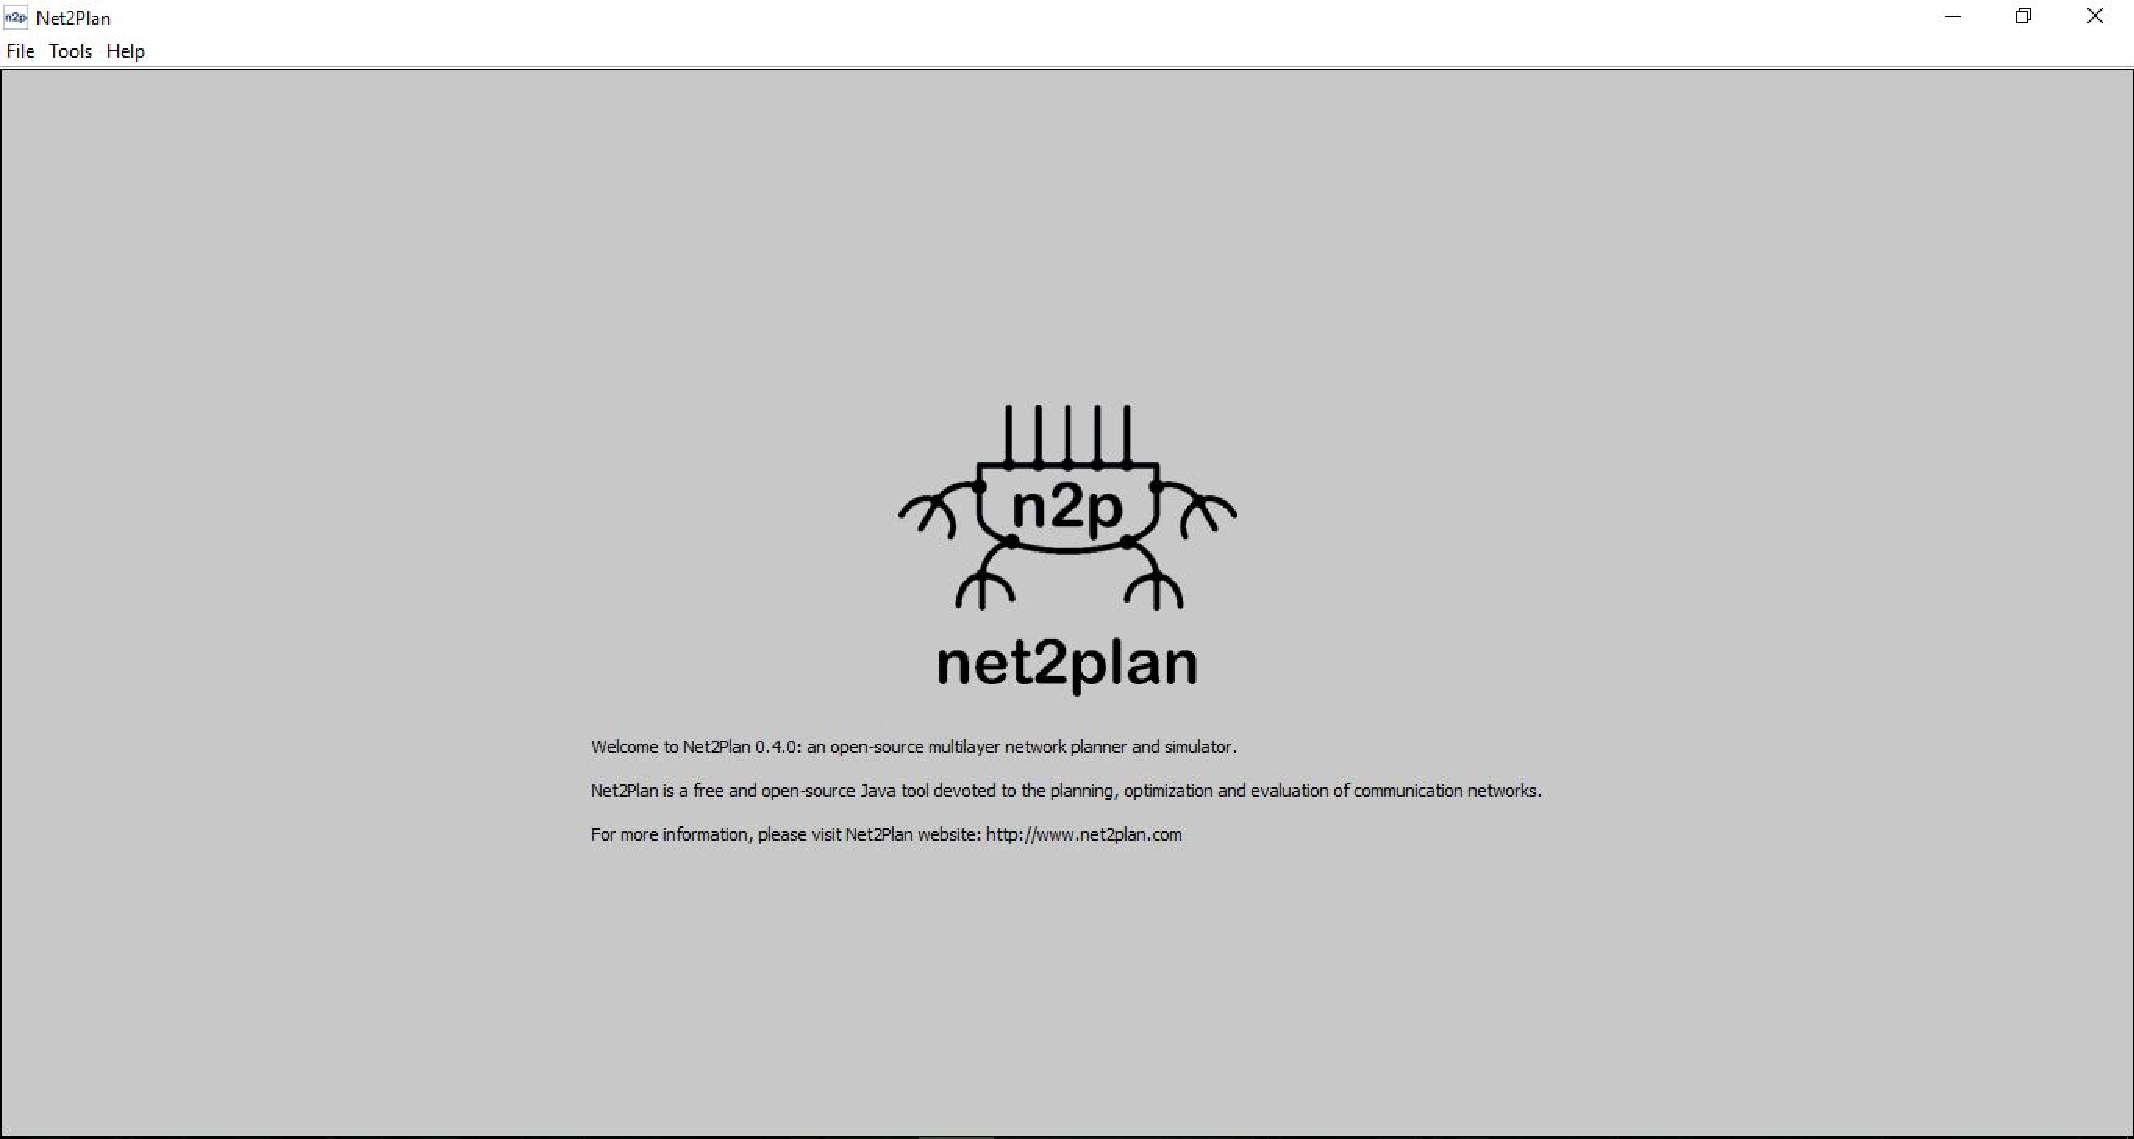
\includegraphics[width = 13cm]{Net2Plan.pdf}
       	\caption{Net2Plan Opening Menu}
    \end{figure}

	\subsection*{Net2Plan Options and installing solvers}
	\vspace{0.5cm}
	To access the main Net2Plan options click "File $\rightarrow$ Options". In this window the global parameters for simulations can be changed if needed.
	For example, an important option to note in this tab is the parameter "defaultRunnableCodePath", whose value should be the path to the jar file containing NetPlanner algorithms. As will be explained further on, Net2Plan is an open source tool and as such, new algorithms can be implemented and the default path can be changed to the path where those will be available instead of loading them manually each time Net2Plan is opened.	The remaining parameters are related to solver options, which are the default external solvers used and also the path in which the $".dll"$, $".so"$, $".dylib"$ files of each solver are available. By default there is no path for each solver but in this case it was already changed to where the solvers were installed.
	\pagebreak
	
	\begin{figure}[h!]
		\centering
		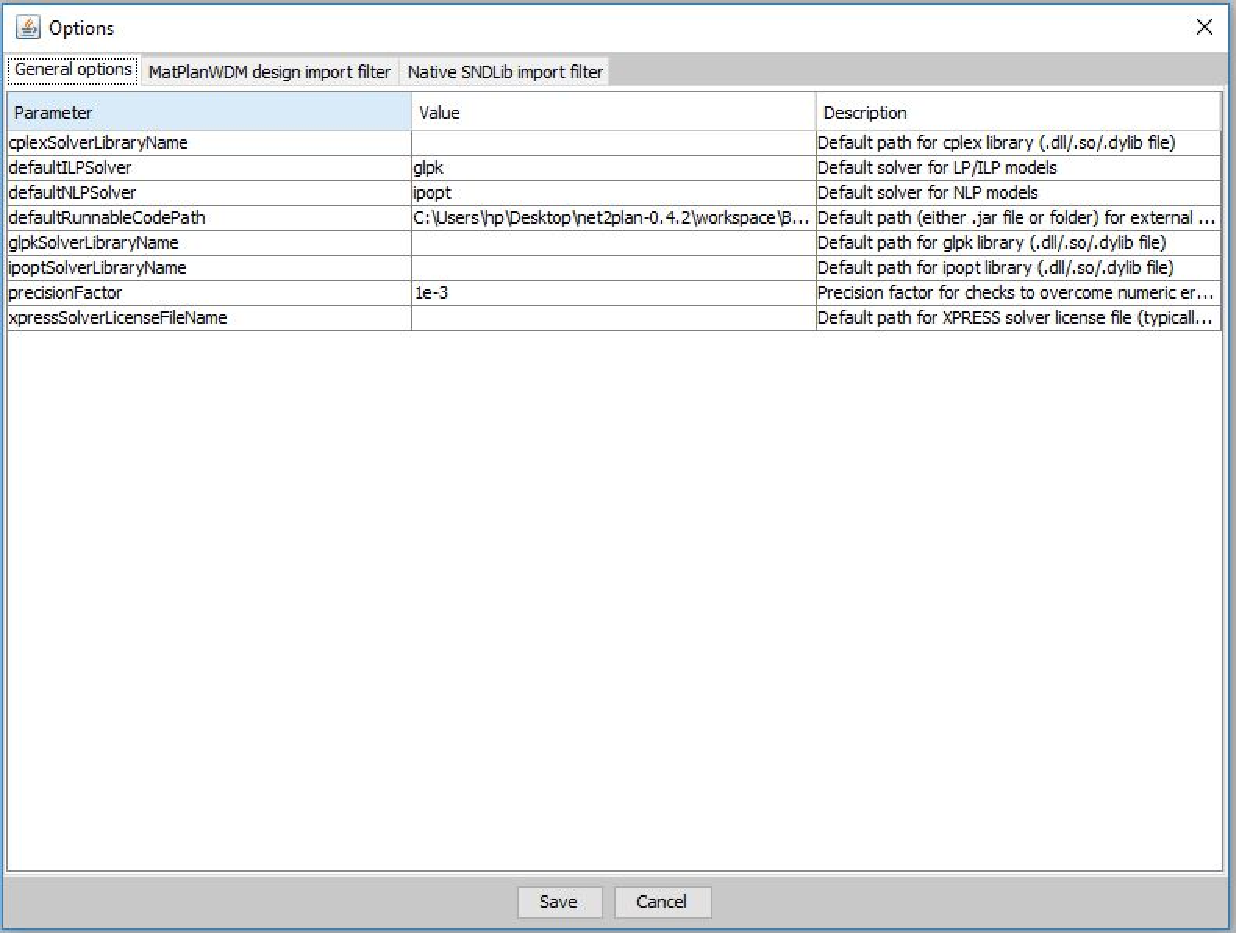
\includegraphics[width = 11cm]{Net2Plan_options.pdf}
		\caption{Net2Plan General Options}
	\end{figure}
		
	
			
	These external solvers are not extracted along with Net2Plan and as such, need to be downloaded if needed for the algorithms to be used. As "cplex" is a paid application, only the other two solvers will be shown as the process is similar.\\
		
	The "IPOPT" solver can be downloaded from \url{http://www.coin-or.org/download/source/Ipopt/}. There are various choices available to download but for this case the $.dll$ is the main file needed. An example of an algorithm which uses this solver is shown on Figure \ref{Net2Plan_ipopt}. Note that the "solverLibraryName" has the path shown earlier on the "Solver options" tab, this would have to be added manually if not introduced into the main options.
	
		
	\begin{figure}[h!]
		\centering
		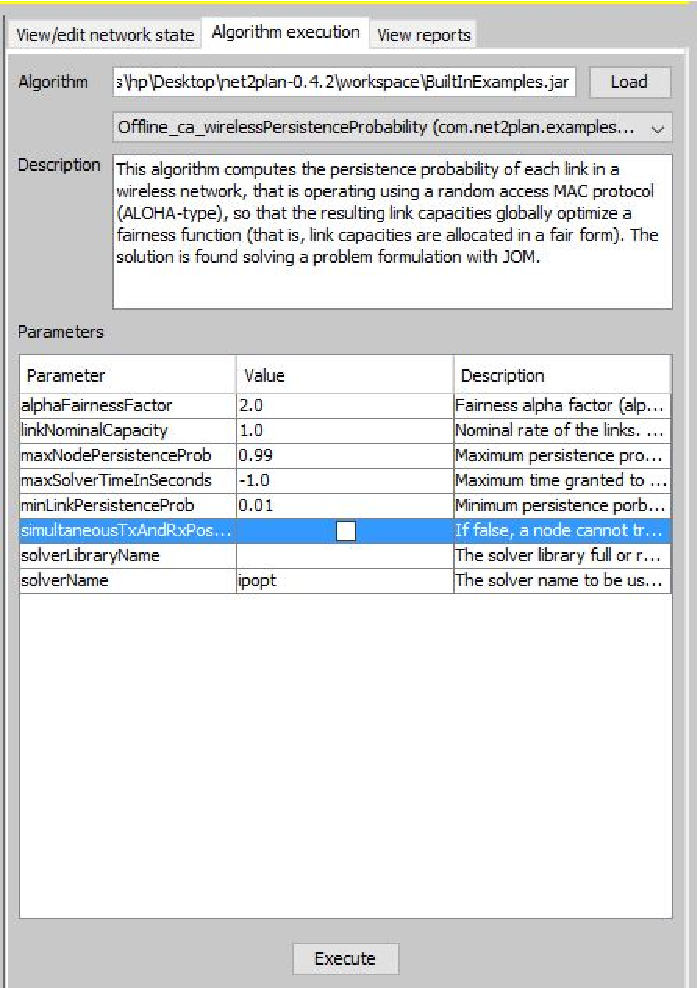
\includegraphics[width = 7cm]{Net2Plan_ipopt.pdf}
		\caption{Net2Plan Algorithm with $ipopt$ solver}
		\label{Net2Plan_ipopt}
	\end{figure}
				
	\vspace{-0.2cm}
		
	The other free solver also used by some Net2Plan is "glpk", this one can be downloaded from \url{http://sourceforge.net/projects/winglpk/?source=typ_redirect}. An example is shown on Figure \ref{Net2Plan_glpk}. Again note the path shows up as in the options.
		

		
	\begin{figure}[h!]
		\centering
		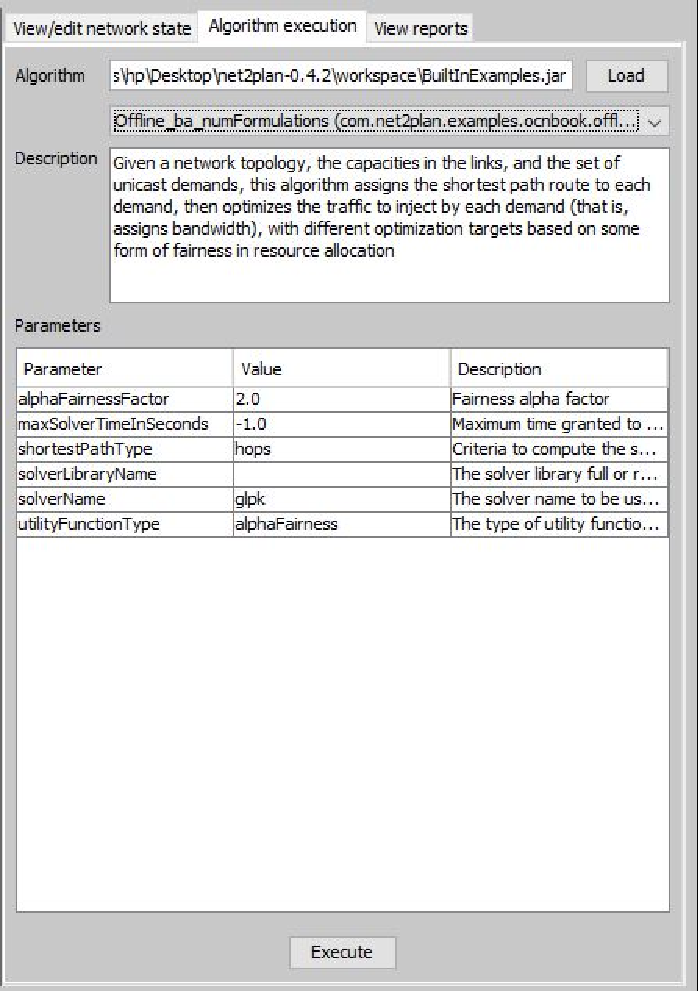
\includegraphics[width = 7cm]{Net2Plan_glpk.pdf}
		\caption{Net2Plan Algorithm with $glpk$ solver}
		\label{Net2Plan_glpk}
	\end{figure}		
		   	
    \newpage

\section*{Net2Plan Tools}
This section will describe in some detail the tools presented in Net2Plan as a network planner, most notably how to created a traffic matrix, design a network and some of the simulation options available.

	\subsection*{Creating Traffic Matrices}
    To start creating a traffic matrix in Net2Plan go to "Tools $\rightarrow$ Traffic matrix design" or press $Alt+2$. The traffic matrix menu is shown on Figure \ref{Net2Plan_traffic}.
	
	\begin{figure}[h!]
		\vspace{-0.3cm}
		\centering	
		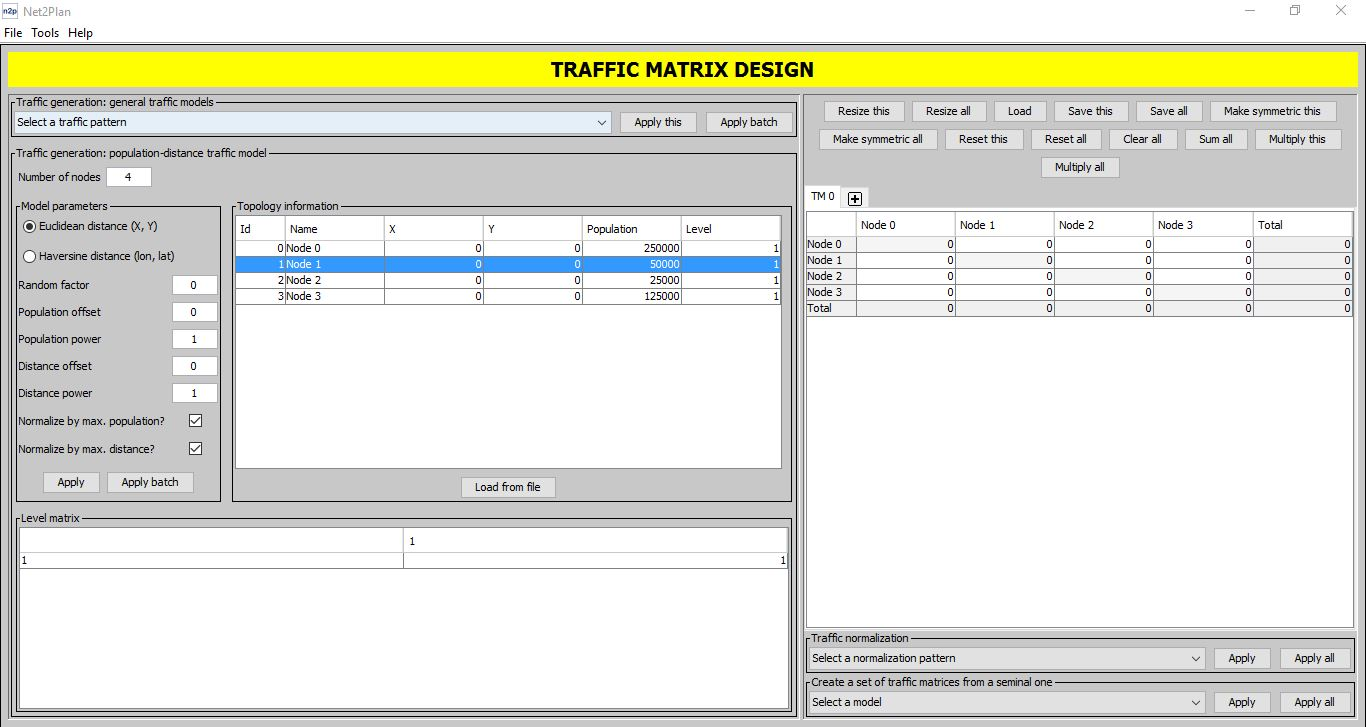
\includegraphics[width = 16cm]{Net2Plan_traffic.pdf}
		\caption{Net2Plan Traffic Matrix Design}
		\label{Net2Plan_traffic}
	\end{figure}
		
	\vspace{-0.3cm}
	
	On the top left side a traffic pattern can be chosen for one matrix or several if used the "Apply batch" option.
	
	\begin{itemize}	
		
		\item{"Constant" has two parameters the number of nodes and a constant value. This creates an uniform matrix with the number of nodes chosen and traffic equal to the value selected.}
	
		\item{"Uniform (0,10)" has the number of nodes and the option of being symmetric as the parameters. The matrix then has the number of nodes introduced and an amount of traffic chosen randomly between 0 and 10 which can be symmetric or not depending on the choice done.}
	
		\item{"Uniform (0,100)" is very similar to the other uniform option whereas in this case the traffic values are chosen randomly between 0 and 100.}
	
		\item{"50\% Uniform (0,100) \& 50\% Uniform (0,10)" and "25\% Uniform (0,100) \& 75\% Uniform (0,10)" are as expected a mixture of the previous two options.}
	
		\item{"Gravity model" in this option a number of nodes is chosen as well as the amount of traffic both generated and received by each node. The sum of the traffic generated by all the nodes needs to be equal to the sum of the traffic received by them. }

	\end{itemize}
	
	Below the traffic pattern options, an existing model can be loaded and additional parameters defined such as Population and Node Level.
	
	On the right side a traffic matrix can be created manually by defining the number of nodes on "resize this" and the amount of traffic can be typed on each demand. The other options above the matrix are self explanatory, for example, "multiply this" multiplies all the traffic by a constant number chosen. A point to note is that most options has an "all" choice as it is possible to have more then one matrix created.
	
	Below the matrix part are two further options available for the matrices, the first one is the option to select a normalization pattern such as "Total normalization" where a total number of traffic can be chosen for the network and the demands are adapted to it accordingly. The other option is to create a set of matrices based on the designed one.\\
	
	Figure \ref{TrafficMatrixCreation} shows how to create batch of matrices with constant traffic.
	
	\begin{figure}[h!]
		\centering
		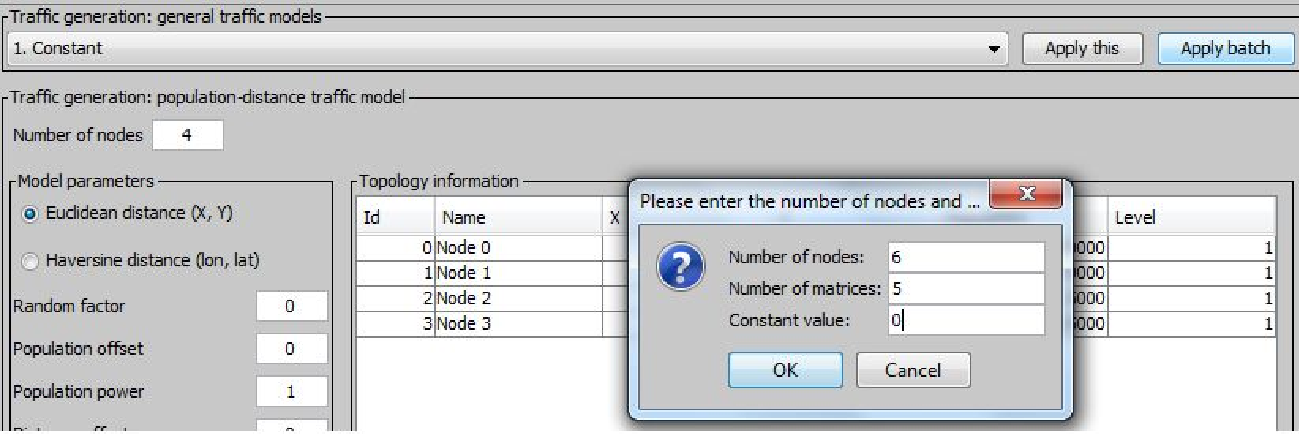
\includegraphics[width = 13cm]{TrafficMatrixCreation.pdf}
		\caption{Net2Plan example on creating a batch of matrices }
		\label{TrafficMatrixCreation}
	\end{figure} 	
	
	Using this option, 5 traffic matrices for a 6 node network were created all with a constant value of 1 as can be seen on figure \ref{Net2Plan_matrix} that shows the first matrix of the batch.

	\begin{figure}[h!]
		\centering
		\includegraphics[width = 13cm]{Net2Plan_matrix.pdf}
		\caption{Net2Plan Traffic Matrix Example}
		\label{Net2Plan_matrix}
	\end{figure}
	
	This example demonstrates how several different types of traffic can be introduced for a network by creating different matrices for each. These can then be saved individually and will further on be used as traffic matrices for ODU's 0 through 4.
	
	\newpage
		
	\subsection*{Creating the Network topologies} \label{Creating the Network topologies}
	To start with the Network creation tools in Net2Plan go to "Tools $\rightarrow$ Offline network design" or press $Alt+1$. The network design menu is shown on Figure \ref{Net2Plan_Network}.
	
	\begin{figure}[h!]
		\centering
		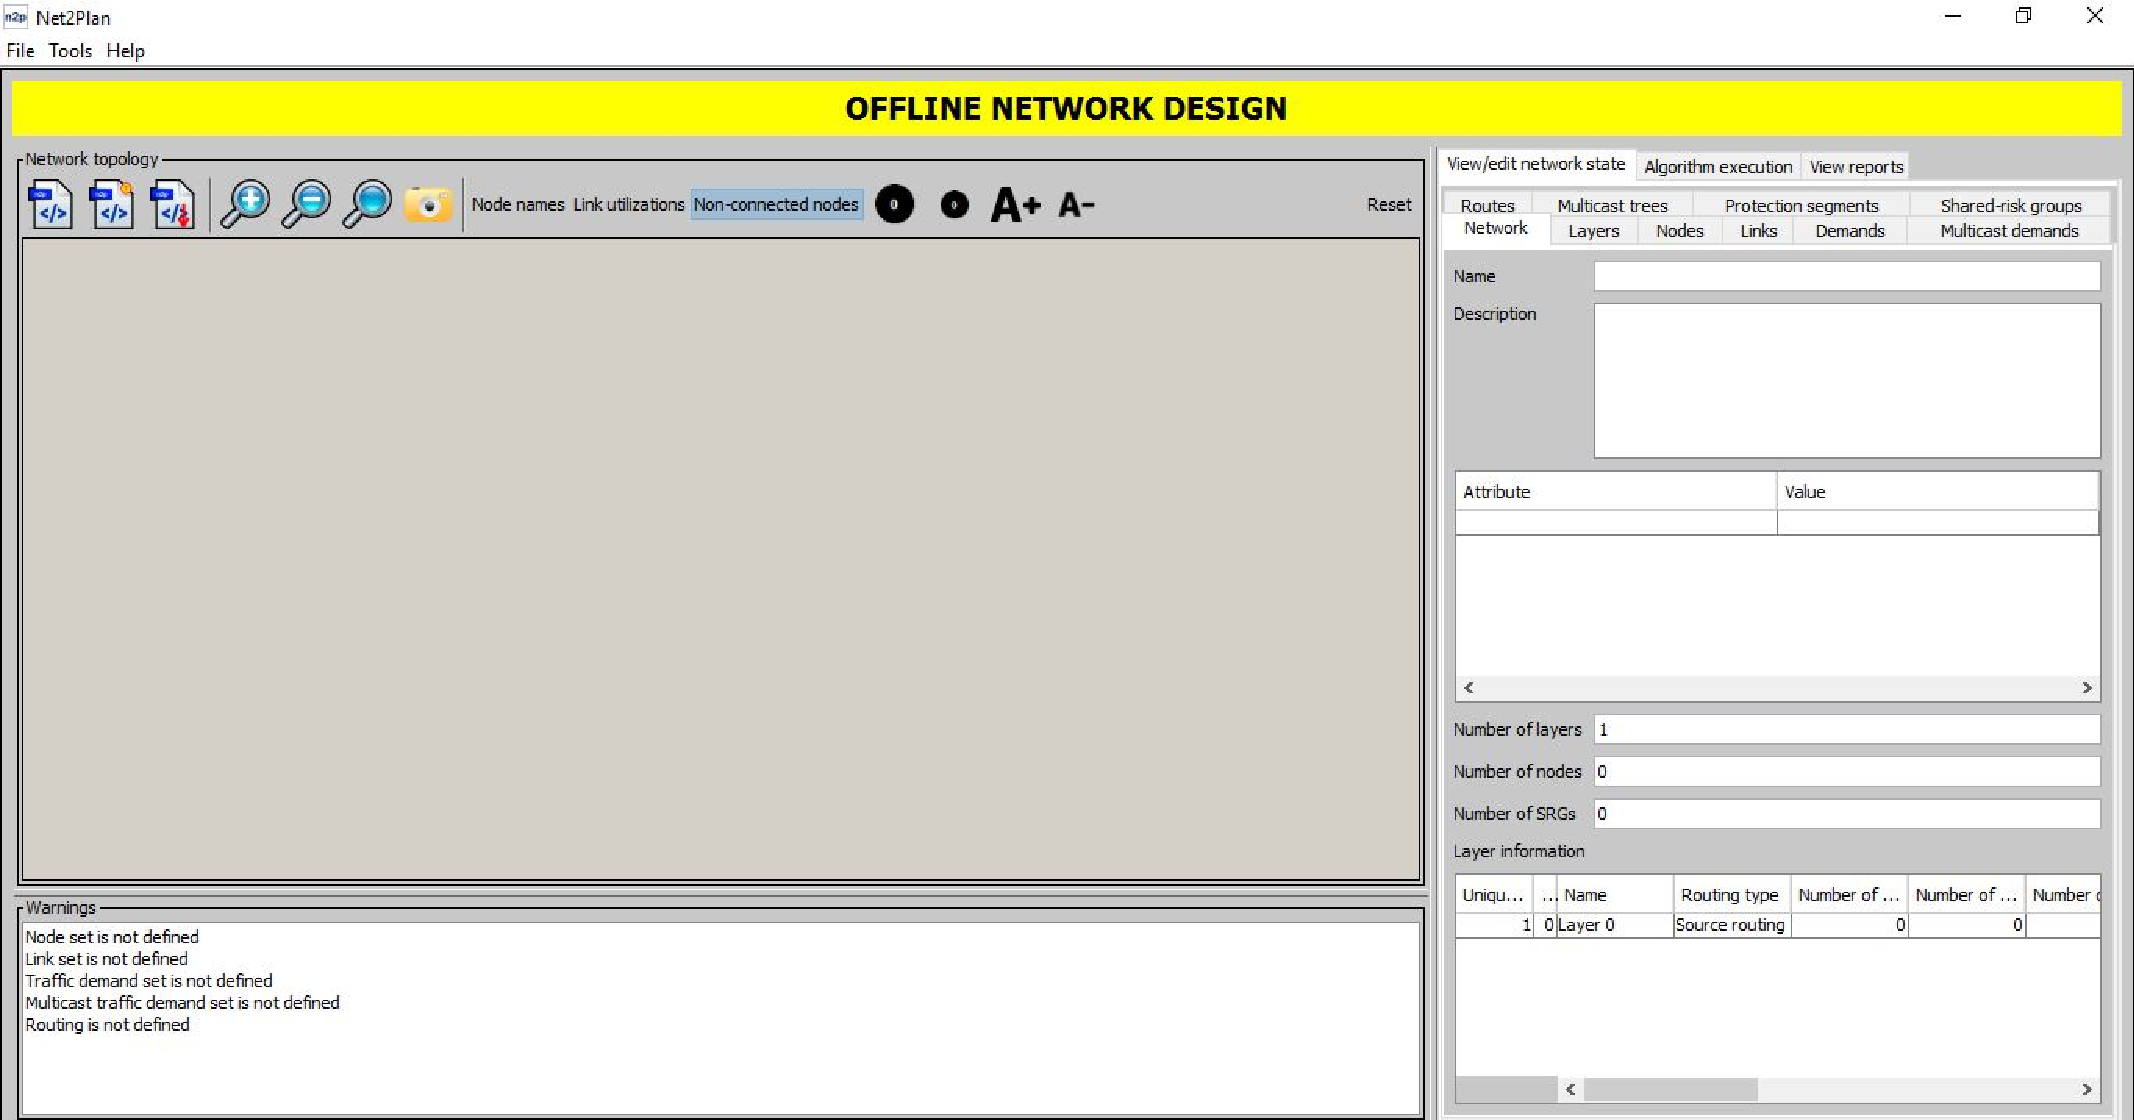
\includegraphics[width = 17cm]{Net2Plan_Network.pdf}
		\caption{Net2Plan Offline Network Design}
		\label{Net2Plan_Network}
	\end{figure}
	
	On the left side, the network topology part has the option to load an existing design and demand set or a new one can be created. To start creating a new network, first nodes have to be introduced by right clicking on the grey area and choosing "Add node here". Links between nodes are created by holding a click on the origin node and dragging until the destination node, holding shift before releasing the click creates 2 links, one in each direction. Another option to create links is to right click on an existing node and choosing the desired create a link option. Nodes can be moved by holding control and dragging them into the desired position.\\
	
	Below the network topology is the "Warnings" box where the parts missing from having a functional network are displayed. For example if the nodes and links where already created it should say "traffic demand set is not defined" and "Routing is not defined" as these were still not introduced.\\
	
	The whole right side of the network design menu are the parameters separated into various tabs which will be explored further on in this document. Besides these tabs, there is also the tab for Algorithm execution where the network is modified based on built algorithms, for example a routing algorithm and the View reports tab where information on the network can be displayed from built in reports. \\

	Figure \ref{Net2Plan_Network_1} demonstrates an example of the 6 node and 16 links network created using the tools explained above. As can be seen on the image at the warning tab, this network sill has several steps left to become a fully functional network. The link capacity will be defined based on the routing algorithm chosen and the demand set will be loaded based on the matrices created. \\
		
	\pagebreak
	\begin{figure}[h!]
		\centering
		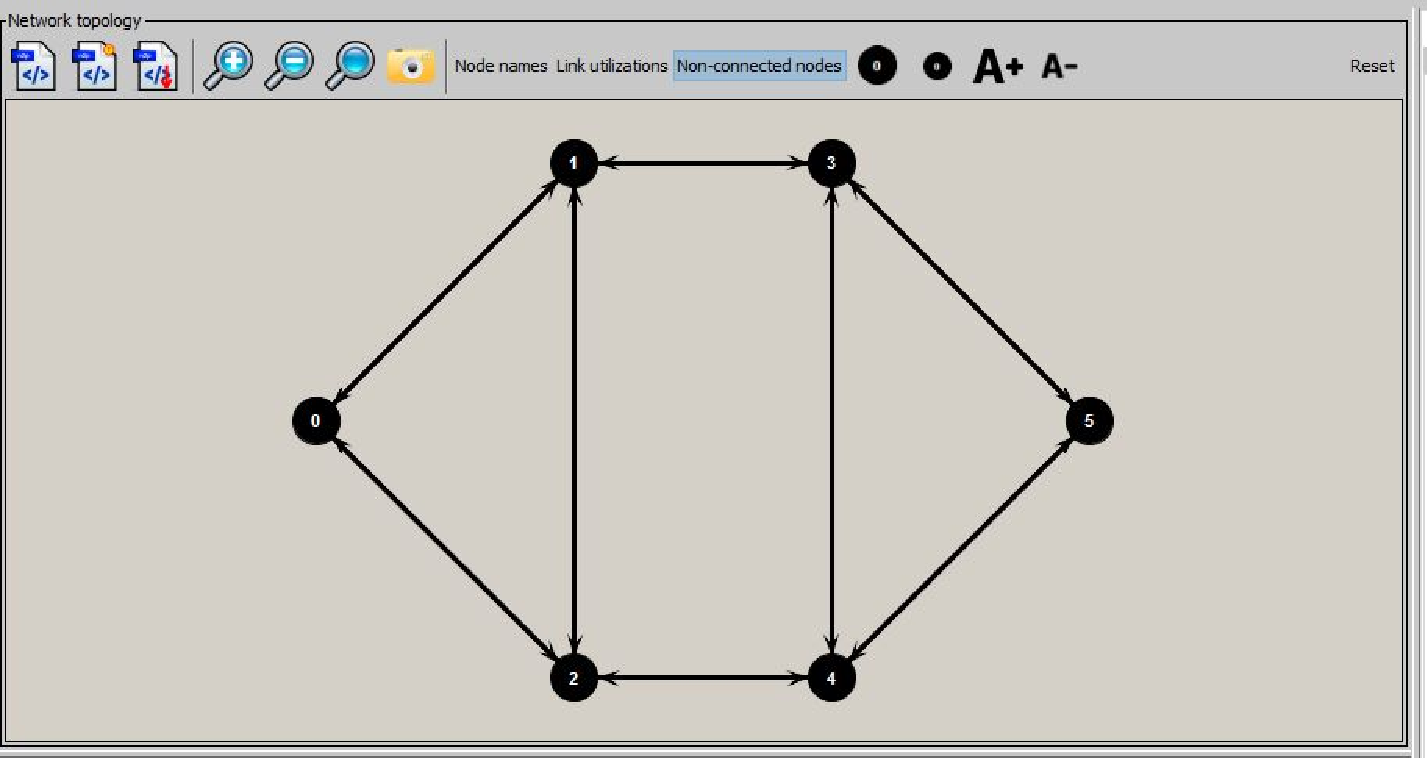
\includegraphics[width = 12cm]{Net2Plan_Network_1.pdf}
		\caption{Net2Plan Network Example}
		\label{Net2Plan_Network_1}
	\end{figure}

	The links and nodes parameters created for the network can be visualized and modified as seen on Figures \ref{Net2Plan_Network_Parameters_a} and \ref{Net2Plan_Network_Parameters_b} displaying the tabs for each case.
	

	\begin{figure}[!h]
		\centering
		\subfigure[a]
		{
			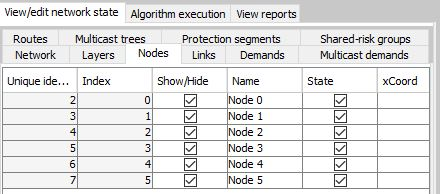
\includegraphics[width=8cm]{Net2Plan_Network_Parameters.pdf}
			\label{Net2Plan_Network_Parameters_a}
		}
		\subfigure[b]
		{
			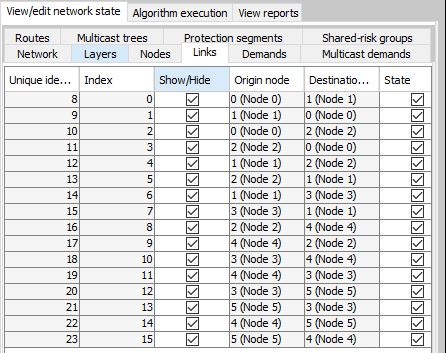
\includegraphics[width=8cm]{Net2Plan_Network_Parameters_1.pdf}
			\label{Net2Plan_Network_Parameters_b}
		}
		\caption{Network a) Nodes tab ; b) Links tab}
	\end{figure}	
	
	On the Nodes tab most of the parameters are still 0 as there is no traffic on the network but there are three parameters that can be changed here. A node name can be set and both x and y coordinates can be defined as a more thorough alternative to define the node position.
	
	On the links tab, again most is at 0 at this moment while the parameters that can be manually set are the link capacity, at 0 until defined and the link length which was set to the same value in every link.\\
	
	Having the basic physical topology created, the next step is to load the demand set into the network. In the case where there are multiple traffic matrices an algorithm was developed to aggregate these in order for it to be possible to load all demands.
	For traffic matrices with ODU signals, an algorithm called "joinTrafficMatrices" can aggregate the different ODUs and convert them to ODU0 in order to have all the traffic in the same units. Besides converting the different ones to ODU0 it also creates an attribute in each demand indicating the type of signal before converting. This attribute can be seen on the demands tab after loading the resulting demand list. Figure \ref{joinMatrices} shows the algorithm to be used.
	

	\begin{figure}[h!]
		\centering
		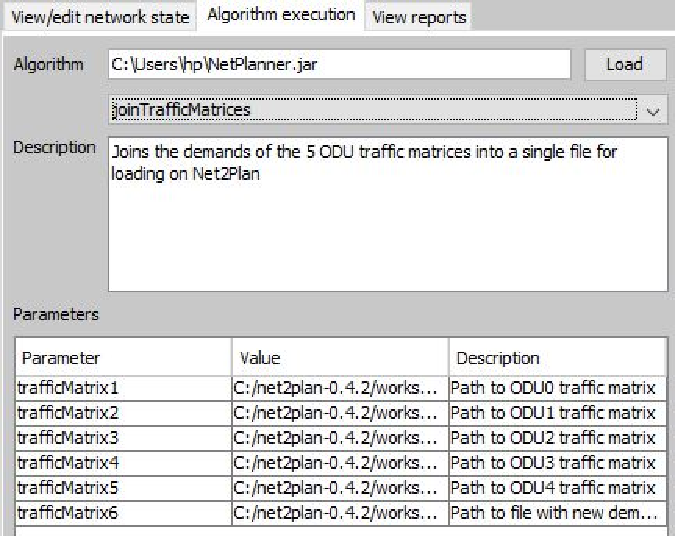
\includegraphics[width=11cm]{Net2Plan_joinMatrices.pdf}
		\caption{joinTrafficMatrices Algorithm}
		\label{joinMatrices}		
	\end{figure}
	
	As can be seen on Figure \ref{joinMatrices} there are 6 user defined parameters, the first five are the paths for the traffic matrices to be aggregated in order, as said in the description. The last parameter is the resulting demand list that can then be loaded into the network.
	
	The paths are by default defined considering Net2Plan is on C:\ and the matrices are in the default directory were they are saved. Lastly, the name of the files are in order ODU0.n2p through ODU4.n2p. All the path and file names can be changed to where the matrices are saved taking into account that just the order of the ODUs needs to be kept due to the conversion to ODU0 units.\\
	
	To load the resulting demands into the created network the second icon on top of the network topology called "Load a demand traffic set" is used. After this, the warning tab changes from "Traffic demand set not defined" to "Traffic losses: Not all the traffic is being carried". This new warning indicates that the demand are in the network but as the routes have not yet been defined the traffic is not being transported.\\
	
	In the demands tab, all the traffic that was created will be displayed in order of ODU type. For this case as all matrices were unitary and uniform, there are thirty demands with offered traffic 1 which is the ODU0 matrix and then consecutively groups of 30 demands (6 nodes) with offered traffic based on the ODU type (5 matrices). For example, an ODU1 is equivalent to two ODU0 so these demands have 2 in offered traffic and an attribute called ODU with value 1.\\
	
	\pagebreak
	
	Before going into the network routing, the network transport mode needs to be defined by creating a logical topology. An algorithm was developed that creates a new layer consisting on this topology depending on the transport mode chosen. This algorithm can be seen on Figure \ref{Logical_Topology_Algorithm}.\\
	
	
	\begin{figure}[h!]
		\centering
		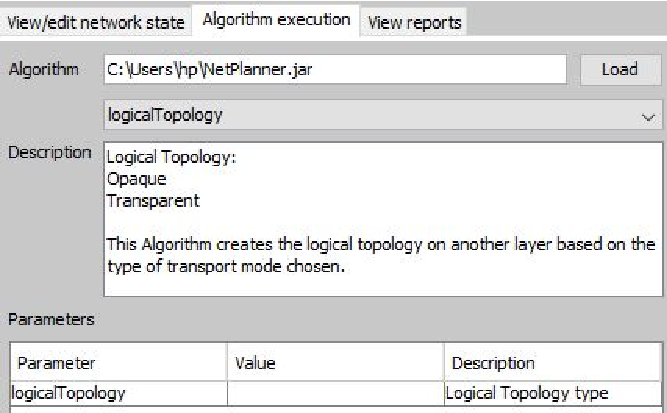
\includegraphics[width = 11cm]{Logical_Topology_Algorithm.pdf}
		\caption{Net2Plan Logical Topology Algorithm}
		\label{Logical_Topology_Algorithm}
	\end{figure}	
	
	There are two user defined parameters on this algorithm. The "logicalTopology" parameter defines the type of transport mode, Opaque or Transparent.\\
	
	%The other parameter, "maximumOpticalReach" is only needed for the Translucent transport mode to define the distance between OEO (Optical-Electrical-Optical) conversions.
	
	Besides creating this new Layer, the algorithm also copies the demands to that layer and defines the logical links based on the length of the physical ones.
	Figures \ref{Net2Plan_Opaque}, \ref{Net2Plan_Transparent}  demonstrate the resulting logical topologies for each transport mode.
	
			\begin{figure}[!h]
				\centering
				\subfigure[]{
					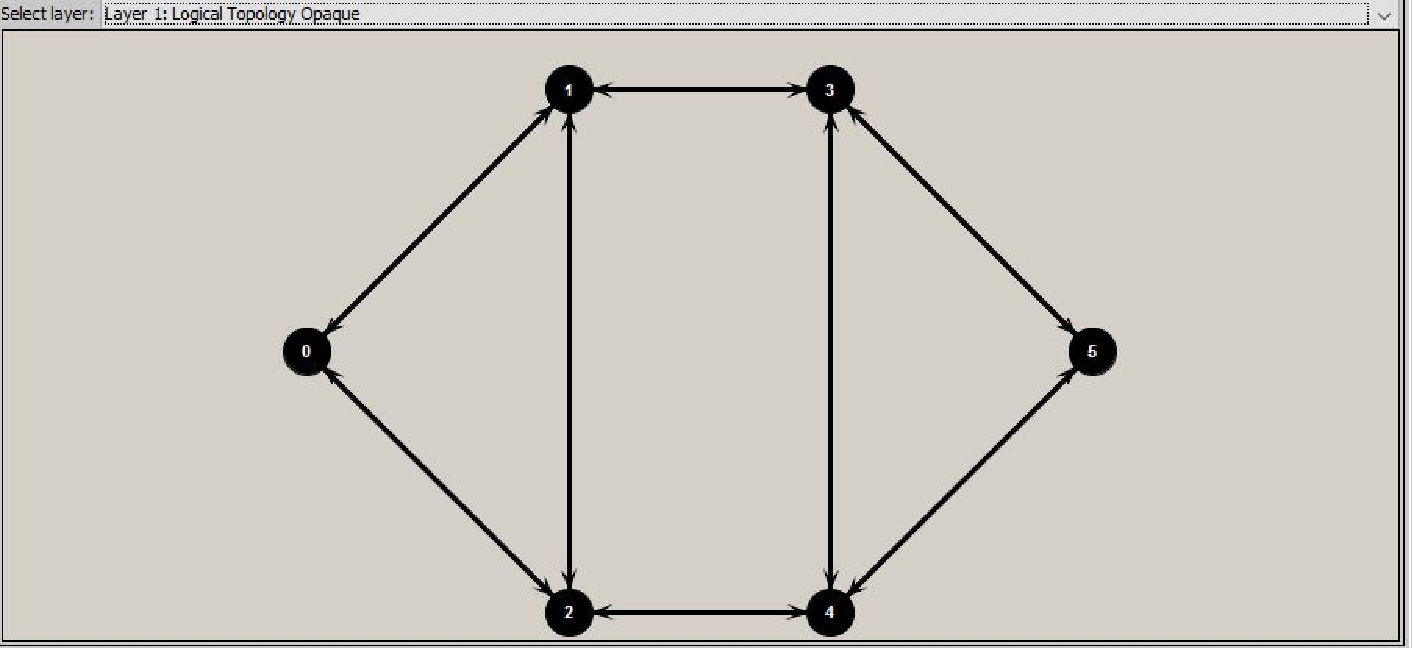
\includegraphics[width=7cm]{Net2Plan_Opaque.pdf}
					\label{Net2Plan_Opaque}					
				}
				\subfigure[]{
					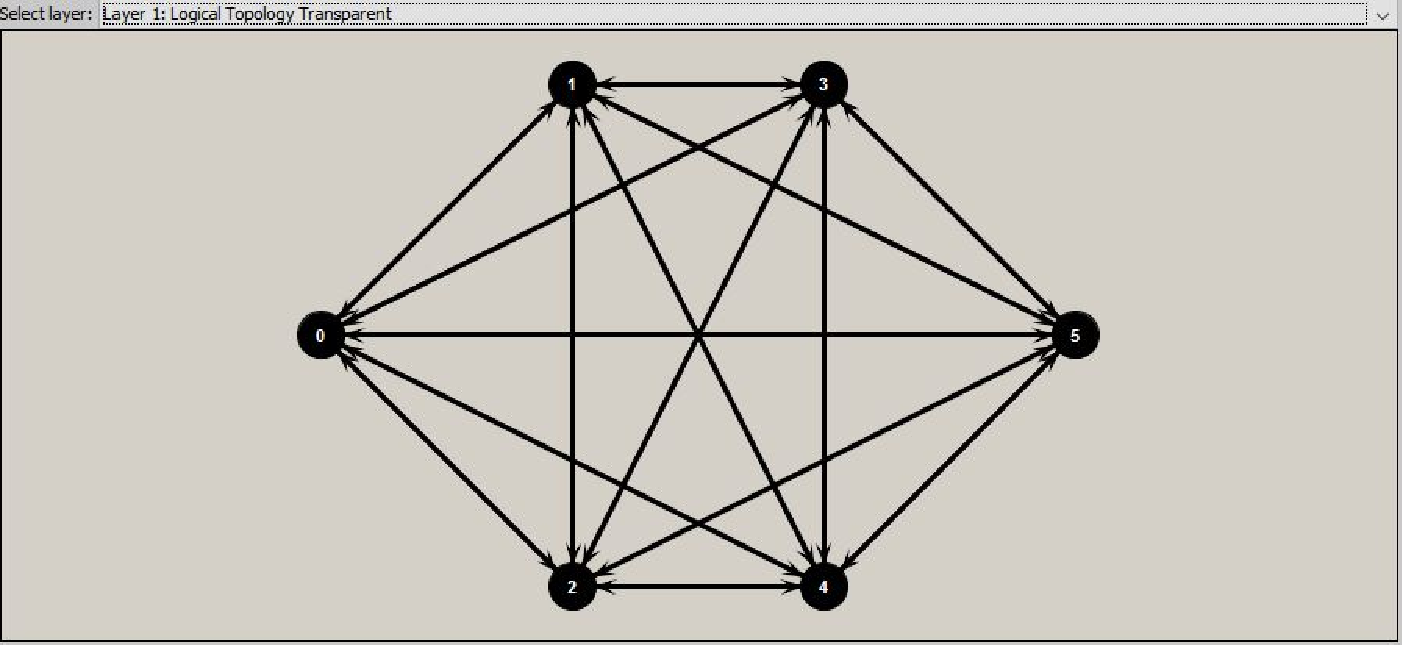
\includegraphics[width=7cm]{Net2Plan_Transparent.pdf}		
					\label{Net2Plan_Transparent}									
				}
				
				\caption{Logical Topology: a) Opaque; b) Transparent;}								
			\end{figure}	

	As can be seen on the logical topologies, for an Opaque transport mode the traffic goes through an OEO conversion at every node and as such the logical topology is the same as the physical one.
	
	In the Transparent mode, there are no regeneration in intermediate nodes and as such the logical topology shows that the traffic between nodes flows directly without grooming with signals from another source.
	
	%Lastly for the Translucent mode, the grooming is performed in a mix between the previous two modes. Up to a certain reach defined in the logical topology algorithm the network acts similarly to a transparent one and after that distance the signal is regenerated as in an Opaque network. For the example presented the optical reach was 400 km.
	\pagebreak
	\subsection*{Routing and Grooming} \label{Routing and Grooming}
	In this section, different routing and grooming options will be discussed for both a network without protection and using a 1+1 protection scheme (dedicated path protection).\\
	The routing will be done based on a shortest path algorithm where the routes for each demand are are created based one either the shortest number of hops needed to reach the destination node or by shortest distance in km. The option can be chosen as a user defined parameter on the algorithm as can be seen on Figure \ref{Grooming_Algorithm}. This algorithm does the routing in both the logical and physical topologies based on the transport mode chosen and makes sure routes are bidirectional meaning the route from node $o$ to $d$ should be the opposite direction of node $d$ to $o$ as there could be different routes with the shortest path that are not using the same path.
	
	\vspace{0.5cm}
	\begin{figure}[h!]
		\centering
		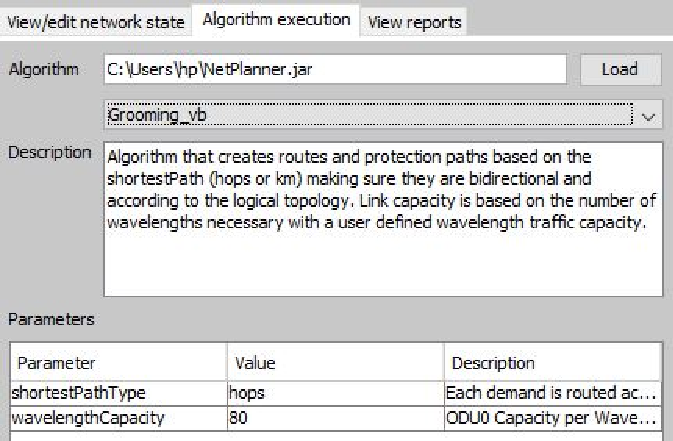
\includegraphics[width = 11cm]{Grooming_Algorithm.pdf}
		\caption{Net2Plan Grooming shortest Path Algorithm}
		\label{Grooming_Algorithm}
	\end{figure}	
	
	Besides the metric through which the shortest path is calculated, the other available parameter defines the amount of ODU0s each wavelength is capable of carrying. By default it is set for 80 ODU0s as it is equal to an ODU4 or 100 Gbit/s.\\

	%The other option for routing without protection is based on reducing the number of wavelengths needed for the network to carry all traffic. Instead of finding the shortest distance between origin and destination node, this algorithm creates the routes based on the previous ones, for example, if the first demand goes through a specific group of links and there is enough capacity in the wavelengths left for the traffic in the next one that demand will be routed to use this spare capacity instead of going through the shortest path.
	
	%As this algorithm is only trying to reduce wasted capacity in links the only user defined parameter available is as before the wavelength capacity in ODU0s, as can be seen on Figure \ref{Grooming2_Algorithm}. The default value is again defined as 80 ODU0s.
		
	%An important point to take into consideration in this algorithm is that even though it might reduce the number of wavelengths needed compared to the shortest path it is not the optimal solution. This fact is due to the limitation imposed by Net2Plan as there is not an option to obtain all available paths between two nodes. The option chosen in order to perform the calculations was to obtain two disjoint paths between the origin and destination node and then performs the steps explained above. This limitation is also felt when creating protection segments in the network as will be explained further on in the 1+1 protection scheme grooming.\\
	
    %\begin{figure}[h!]
	%	\centering
	%	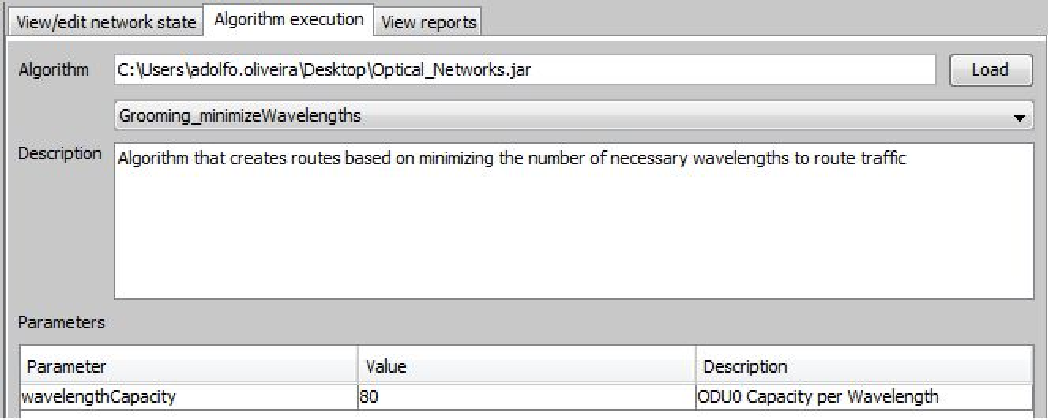
\includegraphics[width = 17cm]{Grooming2_Algorithm.pdf}
	%	\caption{Net2Plan  minimize wavelengths grooming Algorithm}
	%	\label{Grooming2_Algorithm}
	%\end{figure}	
	
	%To create the network routing with a 1+1 protection scheme in place, the algorithms developed for this instance are similar to the ones presented for a network without protection whereas in this case besides finding routes for each demand a protection segment is created with a disjoint path to the one used for the route. "Grooming1\_1" is an algorithm that creates the routes as in the "Grooming" algorithm by choosing the shortestPath and then making the disjoint path the protection one. This algorithm can be run as seen on \ref{Grooming11_Algorithm}.
	
	%\begin{figure}[h!]
	%	\centering
	%	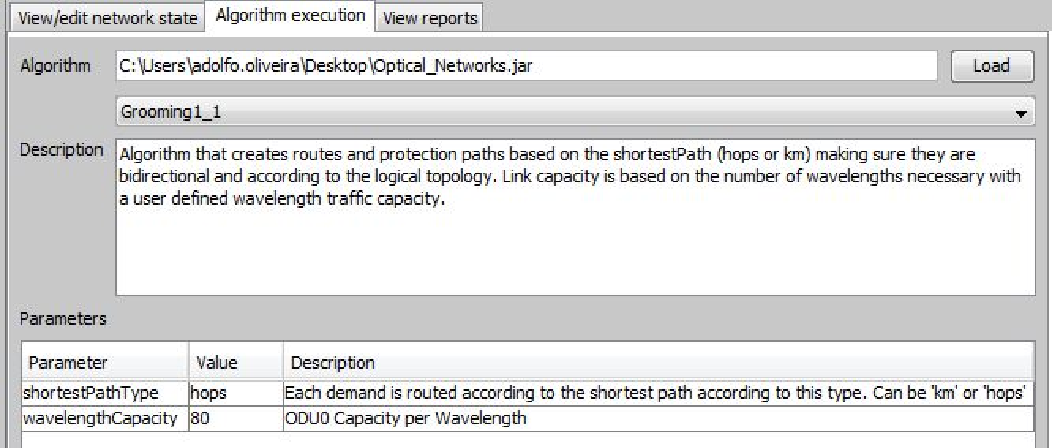
\includegraphics[width = 17cm]{Grooming11_Algorithm.pdf}
	%	\caption{Net2Plan Grooming with protection segments Algorithm}
	%	\label{Grooming11_Algorithm}
	%\end{figure}	
	
	The protection segments similarly to the routes have their own tab where information on their path, route it protects and such can be observed.

\newpage
	
	\subsection*{Reports} \label{Reports}
	As looking separately at each tab to obtain information for different parts of the network is a slow process and does not show some important metrics, Net2Plan allows for the creation of reports where in a similar way to algorithms they can be adjusted to display the information needed, these can also be seen in html format for an easier read. In this section, the report developed will be demonstrated.
	
%   	The first report developed for the optical network classes is called "lineMatrix". This report can be loaded as seen on Figure \ref{lineMatrix_Report}.
%	
%	\begin{figure}[h!]
%		\centering
%		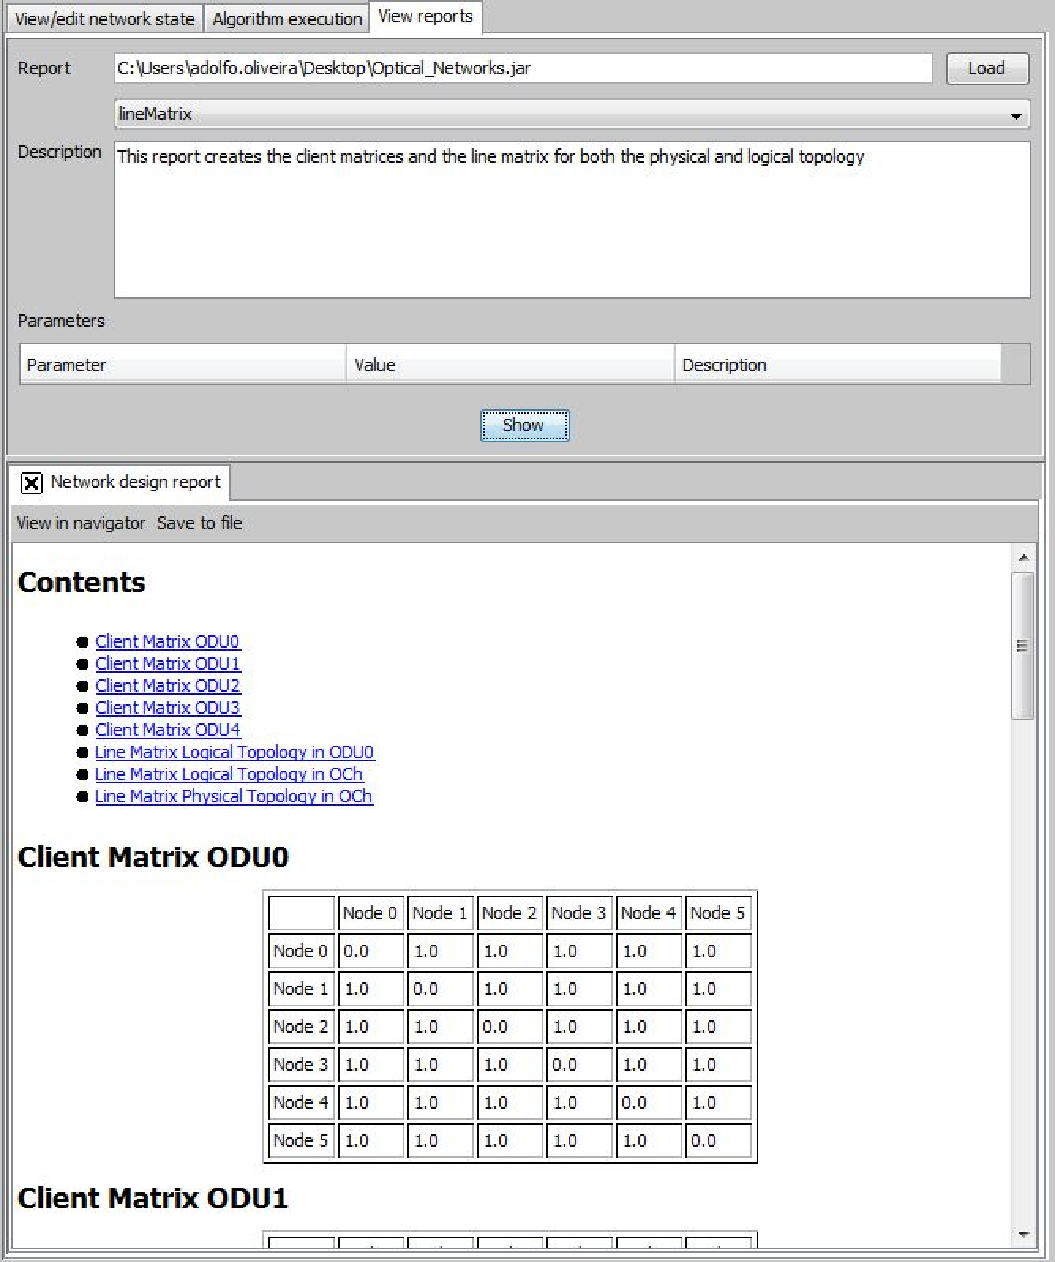
\includegraphics[width=15cm]{lineMatrix_Report.pdf}
%		\caption{Line matrix report}
%		\label{lineMatrix_Report}
%	\end{figure}
%	
%	This report showcases the client matrix created for each ODU type as well as the line matrices in both topologies. In the physical topology the matrix is in Och, number of wavelengths between nodes while on the logical topology there is both a matrix in Och and one in ODU0s.
%	
%	Another report that was created was called "simplifiedReport". This one is a simplified version of the "networkDesign" report whereas in this case only the most relevant information is displayed as can be seen on Figure \ref{simplified_Report}.
%	
%	\begin{figure}[h!]
%		\centering
%		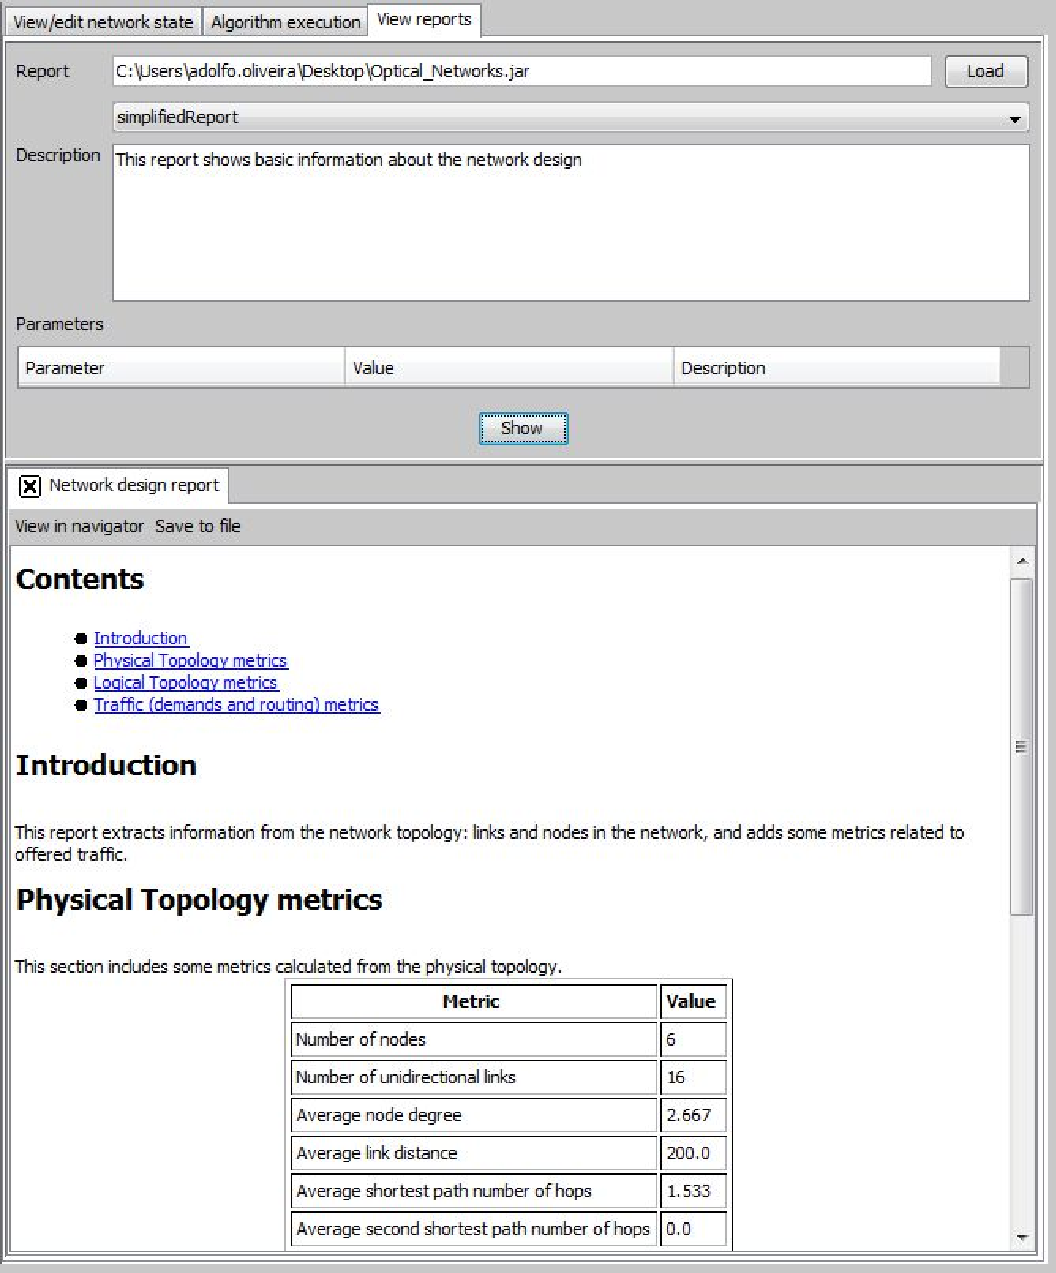
\includegraphics[width=16cm]{simplified_Report.pdf}
%		\caption{Simplified Report}
%		\label{simplified_Report}
%	\end{figure}	
%	
%	Both of these reports have no user defined parameters as they only relay network information. Another option to obtain more network metrics is to use the "Report\_networkDesignModified" as this is a modified version of the already built in Net2Plan report but with a few fixes. This option not only represents the metrics in tables but also has expressions indicating how some of the main network metric can be calculated from basic information. For example the average node degree is obtained by calculating $\frac{E}{N}$.\\
	
	A very important aspect in network planning that is not present natively in Net2Plan is a Network Cost report. To fulfil this gap, a report was created to obtain the network Capex based on user defined equipment costs present on Table \ref{EquipmentCosts}.
		
	\begin{table} [h]
		\centering
		\resizebox{0.4\textwidth}{!}{
		\begin{tabular} {|c|c|}
			\hline
			Equipment & Costs \\
			\hline
			OLT					&	15000\euro		\\ \hline
			Transponder			&	5000\euro/GB	\\ \hline
			Optical Amplifier	&	4000\euro		\\ \hline
			EXC					&	10000\euro		\\ \hline
			OXC					&	20000\euro		\\ \hline
			EXC Port			&	1000\euro/GB/s	\\ \hline
			OXC Port			&	2500\euro/port	\\ \hline										
		\end{tabular}}
		\caption{Equipment Costs}			
		\label{EquipmentCosts}			
	\end{table}
	
	These Equipment costs are introduced into a report as user defined parameters as can be seen on Figure \ref{networkCost_Report}.
	
	\begin{figure}[h!]
		\centering
		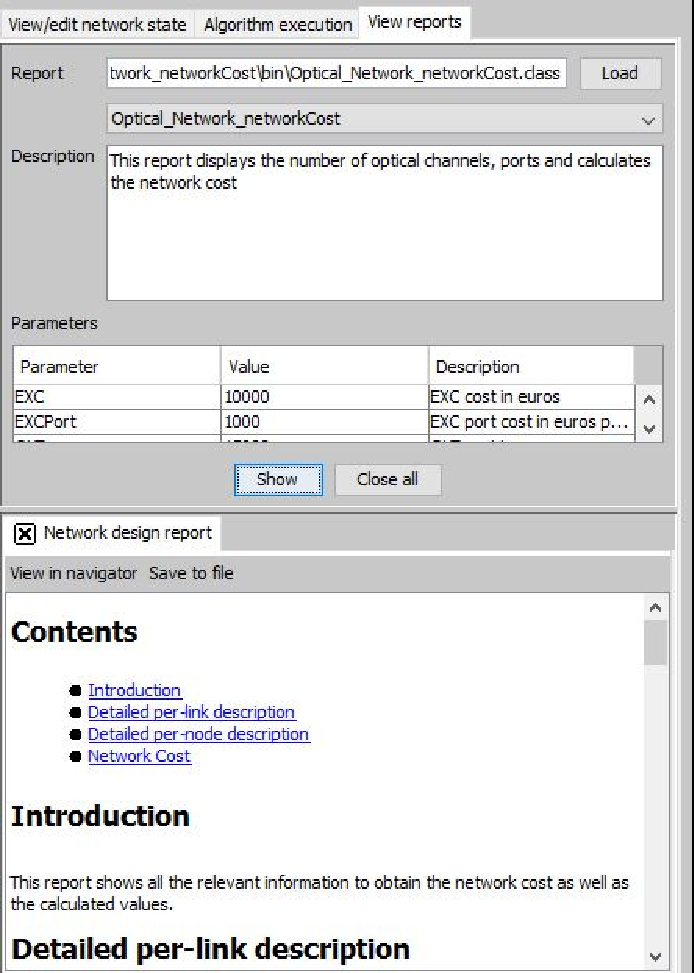
\includegraphics[width=7.5cm]{networkCost_Report.pdf}
		\caption{Network Cost Report}
		\label{networkCost_Report}
	\end{figure}	
	
	Besides the equipment costs, this report also has the parameter "span". The value of this variable is used to calculate the number of optical amplifiers needed in the network using Equation \ref{amplifiersLink}.
	
	\begin{equation}
		N^R = \sum\limits_{l=1}^L\left(\left\lceil\frac{len_l}{span}\right\rceil-1\right)
		\label{amplifiersLink}
	\end{equation}

	The other parameters of this equation being:
	
	\begin{itemize}
		\item{$N^R$			$\rightarrow$ Total number of regenerators/amplifiers}
		\item{$len_l$		$\rightarrow$ Length of link l}
		\item{$span$		$\rightarrow$ Distance between amplifiers}	
	\end{itemize}	
	
	By running the report three main categories are presented to the user.
	
	The first category displayed by the report is the Detailed per-link description. In here the number of optical channels or wavelengths is displayed for each link based on the grooming algorithm used. The numbers displayed are based on the physical topology and represent all the wavelengths that will be needed to transport the network traffic. Using this information it is possible to obtain the average and total number of optical channels on the network.
	
	Besides the number of wavelengths, this section also indicates the amount of amplifiers necessary in each link. \\
	
	The second category is the Detailed per-node description. This section displays a table indicating how many ports are needed of each type for every node. The number of tributary ports obtained in each node is the sum of all traffic originating from that node or ending on it depending if its the input or output ports divided by the amount of traffic each optical channel can carry. This number also depends on the links through which traffic will be routed, for example, if 40 ODU0s are transmitted into 2 separate links only one wavelengths could carry it but as they are going through different routes then 2 wavelengths will be used resulting in also a need for 2 tributary ports.\\
	
	The number of line ports is obtained by adding the total amount of optical channels in the links that use that specific node as origin or destination.\\
	
	Finally the total number of ports is as expected the sum of all the tributary ports with the line ones. With this information the average and the total number of ports in the network can be obtained which will later be used in calculating the network cost.\\
	
	Having the node and link information available, the network cost can then be calculated as displayed on the third category of the report.								
	The Node electrical cost is obtained with Equation \ref{electricalPortsCostTransparent} for a Transparent Network.
	
	\begin{equation}
		C_{exc} = \left(\gamma_{e0}\times N\right) + \left(\gamma_{e1} \times \tau \times 2 \times P_{TRIB}\right)
		\label{electricalPortsCostTransparent}
	\end{equation}
	
	\begin{itemize}
		\item{$C_{exc}$		$\rightarrow$	Electrical Ports Cost}
		\item{$\gamma_{e0}$	$\rightarrow$	EXC cost in Euros}
		\item{$N$			$\rightarrow$	Number of Nodes}
		\item{$\gamma_{e1}$	$\rightarrow$	EXC port cost in Euros per GB/s}
		\item{$\tau$		$\rightarrow$	Traffic supported by optical channel}
		\item{$P_{TRIB}$	$\rightarrow$	Number of tributary ports}
	\end{itemize}
	
	The cost values can be obtained from Table \ref{EquipmentCosts}, the number of nodes is a known value when designing a network, the traffic supported by optical channel is defined by the grooming algorithm or by dividing the link capacity by its amount of optical channels and the number of tributary ports was obtained on the previous section of the report. \\
	
	For an Opaque network, the electrical nodes cost is similar as displayed in Equation \ref{electricalPortsCostOpaque}.\\
	
	\begin{equation}
	C_{exc} = \left(\gamma_{e0}\times N\right) + \left(\gamma_{e1} \times \tau \left(P_{LINE} + P_{TRIB}\right)\right)
	\label{electricalPortsCostOpaque}
	\end{equation}	\\
	
	The node optical cost on the other hand, can be calculated for a Transparent network using Equation \ref{opticalPortsCost}.
	
	\begin{equation}
		C_{oxc} = \left(\gamma_{o0} \times N \right) + \gamma_{o1} \times  \left(P_{LINE} + P_{TRIB}\right)
		\label{opticalPortsCost}
	\end{equation}	
	
	\begin{itemize}
		\item{$C_{oxc}$		$\rightarrow$	Optical Ports Cost}
		\item{$\gamma_{o0}$	$\rightarrow$	OXC cost in Euros}
		\item{$N$			$\rightarrow$	Number of Nodes}
		\item{$\gamma_{o1}$	$\rightarrow$	OXC port cost in Euros}
		\item{$P_{TRIB}	$	$\rightarrow$	Number of tributary ports}
		\item{$P_{LINE} $	$\rightarrow$	Number of line ports}
	\end{itemize}
		
	As for the electrical ports, the cost values were previously defined in Table \ref{EquipmentCosts} and as such, only the number of ports is needed. These value were obtained on the second part of the report (Detailed per-Node description). \\
	
	For an Opaque network, the node optical cost is 0 as the ports are all electrical. \\
	
	The Node Total Cost is as expected the sum of both the optical and electrical node costs. \\
	
	The rest of the network cost is from the links. This cost is obtained with Equation \ref{linksCost}.
	
	\begin{equation}
		C_L = \left(\gamma_0^{OLT} \times L\right) + \left(\gamma_1^{OLT} \times \tau \times W\right) + \left(N^R \times c^R\right)
		\label{linksCost}
	\end{equation}	
	
	\begin{itemize}
		\item{$C_L$				$\rightarrow$	Links Cost}
		\item{$\gamma_0^{OLT}$	$\rightarrow$	OLT cost in Euros}
		\item{$L$				$\rightarrow$	Number of unidirectional Links}
		\item{$\gamma_1^{OLT}$	$\rightarrow$	Transponder cost in Euros}
		\item{$\tau$			$\rightarrow$	Traffic per port}
		\item{$W$				$\rightarrow$	Total number of optical channels}
		\item{$N^R$				$\rightarrow$	Total number of optical amplifiers}
		\item{$c^R$				$\rightarrow$	Optical amplifiers cost in Euros}
	\end{itemize}
	
	As in previous equations, the costs are all available in Table \ref{EquipmentCosts}. The total number of optical channels can be obtained by summing the wavelengths in each link on the Detailed per-Link description section. The number of optical amplifiers was calculated previously with Equation \ref{EquipmentCosts}.
	
	The middle part of the equation: $\gamma_1^{OLT} \times \tau \times W$ refers to the Transponders cost while the rest is the "Fiber" and the "OLT" cost.	Lastly the total network cost can be obtained by adding the Links cost with the Nodes cost.\\
	
	\section*{Results}
	This section will display the results obtained using the algorithms and reports previously explained for a network with an Opaque transport mode and for one with Transparent.

	
	\subsection*{Opaque with 1+1 protection}
	%For this case, the difference to the previous example will be as for the case of a transparent network in the creation of a protection segment for each route.
	
	The results will be displayed only in the logical topology as in an opaque network it is the same as the physical one.
	Using the algorithm presented on figure \ref{Grooming_Algorithm} the routes and protection segments are created as well as the grooming. \\
	
	There is not a second algorithm type for wavelengths reduction due to the fact that, that algorithm chooses the best path based on the shortest or disjointed path which in this case both need to be used one for work and one for protection. As such, is difficult to reduce in any instance the shortest path because of the algorithm performance.
	
	The traffic matrix for the reference 6 node network, used for demonstration is shown below.
	
	\begin{figure}[h!]
		\centering
		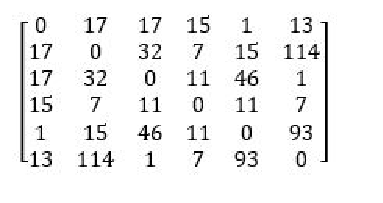
\includegraphics[width=9cm]{opaqueLineMatricesLogical11.pdf}	
		\caption{}
		\label{opaqueLineMatricesLogical11}								
	\end{figure}	
	
	The amount of traffic that needs to be reserved in each link is as was to be expected a lot higher due to the need to reserve double the amount and in more links. The same happens in terms of wavelengths. \\
	
%	Tab layer will display the average number of hops per protection segment as in this case as the other metrics will stay the same. This is shown on Figure \ref{simplifiedReportOpaque11}.
%	
%	\begin{figure}[h!]
%		\centering
%		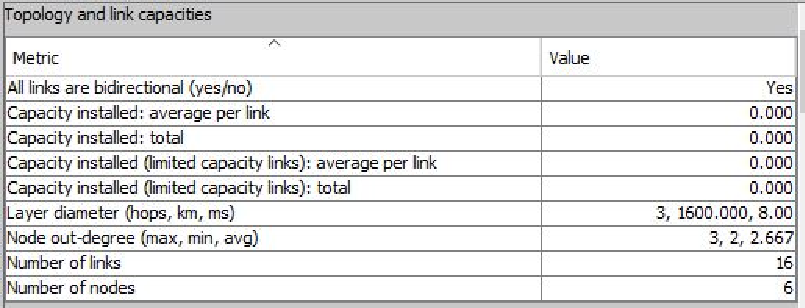
\includegraphics[width=9cm]{simplifiedReportOpaque11.pdf}	
%		\caption{simplified Report for opaque transport mode with 1+1 protection}
%		\label{simplifiedReportOpaque11}								
%	\end{figure}
%	
%	The number obtained for the second shortest path is the same as was obtained in the physical topology in the transparent network since as explained the algorithm being used is the same only difference will be on the way the grooming is done. \\
	
	The number of wavelengths can again be seen on the links section of the "networkCost" report as well as the amplifiers needed on Figure \ref{networkCost_Report_Links_Opaque11}.
	
	\begin{figure}[h!]
		\centering
		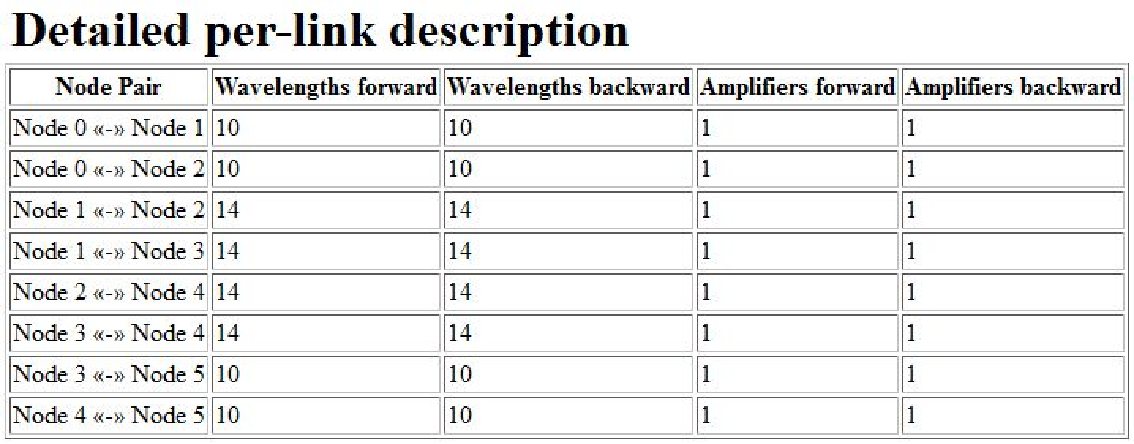
\includegraphics[width=11cm]{networkCost_Report_Links_Opaque11.pdf}	
		\caption{Links for Opaque Network with 1+1 Protection}
		\label{networkCost_Report_Links_Opaque11}								
	\end{figure}	
	
	The conclusions to take from these results are the same as was previously discussed as the number of amplifiers does not change and the wavelengths are the ones shown on the line matrices.
	
	As for the nodes in the network Figure \ref{networkCost_Report_Nodes_Opaque11} shows the ports needed.
	
	\begin{figure}[h!]
		\centering
		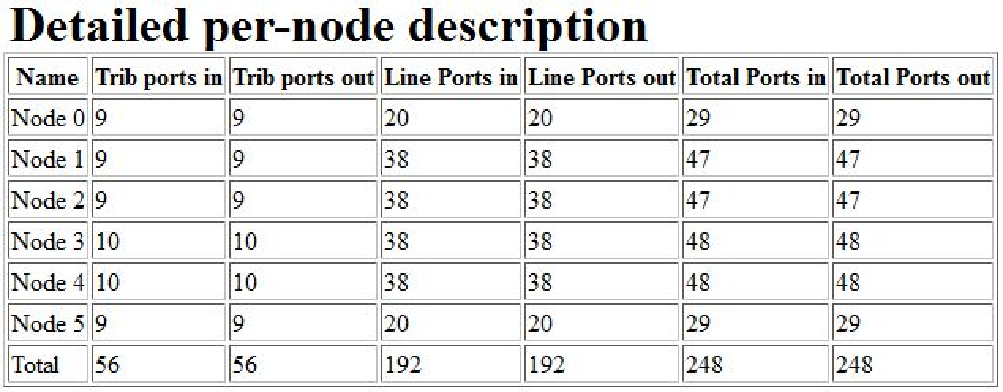
\includegraphics[width=11cm]{networkCost_Report_Nodes_Opaque11.pdf}	
		\caption{Nodes for Opaque Network with 1+1 Protection}
		\label{networkCost_Report_Nodes_Opaque11}								
	\end{figure}		
	
	Again, the difference for the case without protection is only on the number of line ports as this value is based on the number of wavelengths going in or out of that node.
	
	Comparing the number of ports obtained here with the network with a transparent transport mode, the amount is lower for the opaque network due to the reduced number of wavelengths required to route the traffic. \\
	
	Lastly the total network cost is on Figure \ref{networkCost_Report_Cost_Opaque11}.\\
	
	\begin{figure}[!h]
		\centering
		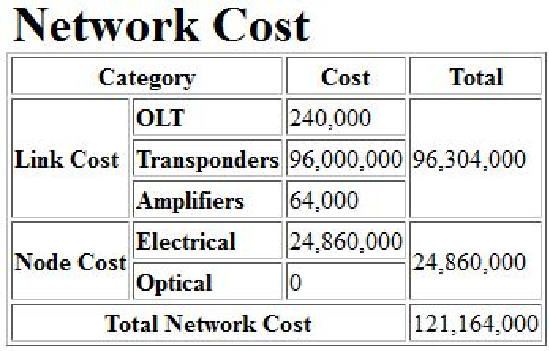
\includegraphics[width=9cm]{networkCost_Report_Cost_Opaque11.pdf}	
		\caption{Network Cost for Opaque Network with 1+1 Protection}
		\label{networkCost_Report_Cost_Opaque11}								
	\end{figure}	
	
	\pagebreak
	
	The increase in cost is as described on the transparent network just based on the additional number of wavelengths required which translates in also more trunk ports needed. As noted above in the amount of ports, the cost is also lower in this instance when compared to the transparent network due to the cheaper cost in transponders and optical ports.
	
	
	
		\subsection*{Transparent with 1+1 protection}
		
		
		For a network with a transparent transport mode, the routing as was explained before, is done using a shortest path algorithm since there are no traffic grooming between different node pairs. For this instance as there is also a 1+1 protection scheme in place, the algorithm needs to not only create the routes but also a protection segment for each route. This segment is the shortest disjoint path of the route created.

		
		Comparing the results obtained here with the previous example, it can be seen that the amount of traffic and wavelengths is significantly higher. It is in both cases, double the amount of before since the same quantity needs to be reserved for protection.\\
		

		
		The conclusions that can be taken from the physical topology are as explained before, the huge number of wavelengths is related to the needed for double the amount of traffic where this extra will go through even more links.
		
		For the logical topology the Average second shortest path number of hops is 1 since as for the shortest path, it is considered that there are always direct links between nodes in a transparent network. As for the physical topology, this value is not so obvious as it has to be calculated based on the second shortest path between each node pair. \\
		
			
	
			
		These differences for the transparent network with protection segments can also be seen on the information provided in the "networkCost" report. Figure \ref{networkCost_Report_Links_Transparent11} shows the results for the links in the physical topology.\\
		
		\begin{figure}[!h]
			\centering
			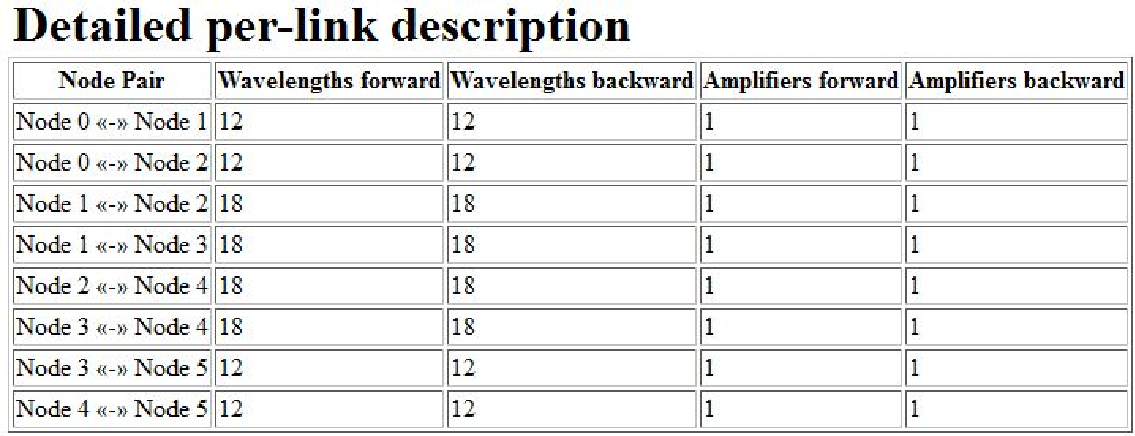
\includegraphics[width=11cm]{networkCost_Report_Links_Transparent11.pdf}
			\caption{Links for Transparent Network with 1+1 Protection}
			\label{networkCost_Report_Links_Transparent11}						
		\end{figure}	
		
		It can be seen that as expected the number of amplifiers is the same due to the link lengths remaining constant but the number of wavelengths are higher due to having a grooming scheme worst with this topology.\\
		\newpage
		The results in terms of ports per node are shown below.
		
		\begin{figure}[!h]
			\centering
			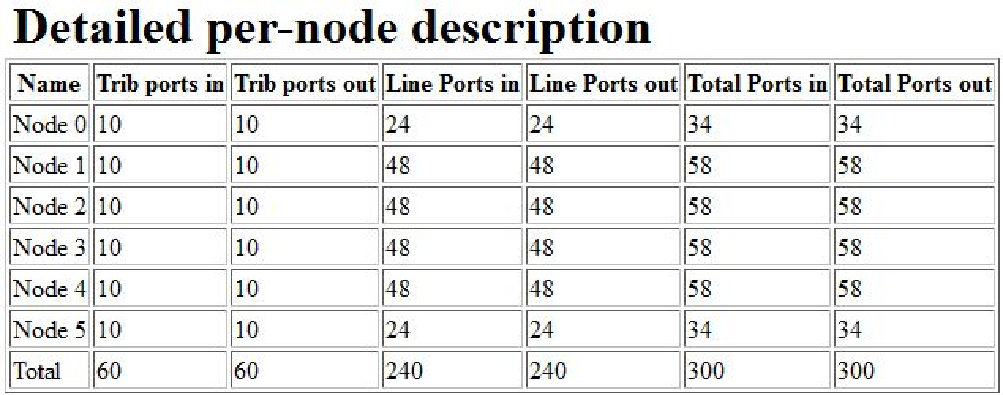
\includegraphics[width=11cm]{networkCost_Report_Nodes_Transparent11.pdf}
			\caption{Nodes for Transparent Network with 1+1 Protection}
			\label{networkCost_Report_Nodes_Transparent11}						
		\end{figure}
		
		 The number of tributary ports remain the same but the number of line ports increase based on the higher number of wavelengths needed in the network.\\
		
		Lastly, the total network cost is shown on Figure \ref{networkCost_Report_Cost_Transparent11}.\\
		
		
		\begin{figure}[!h]
			\centering
			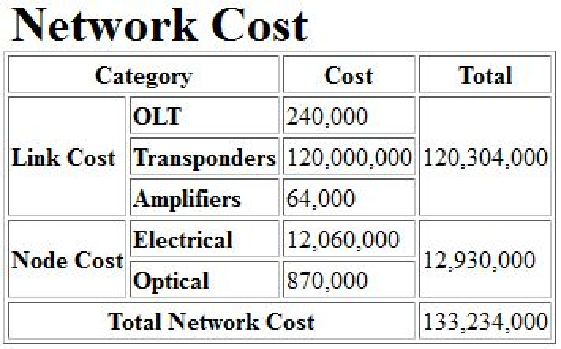
\includegraphics[width=9cm]{networkCost_Report_Cost_Transparent11.pdf}	
			\caption{Network Cost for Transparent Network with 1+1 Protection}
			\label{networkCost_Report_Cost_Transparent11}								
		\end{figure}		
		
		The results obtained for the network Cost confirm those obtained in the previous categories in this report. The OLT and amplifiers cost does not change as the number of links and amplifiers remains the same. Similarly, the electrical ports cost is also the same as the amount of ADD/DROP ports remains the same.
		
		The differences are in the Transponders cost in the links and the Optical cost in the nodes. These as expected, cost more based on the increased number of them needed in the network to have a 1+1 protection scheme in a transparent transport mode network.
		
	
	\newpage
	
	
	\section*{Simulations}
	To access the Simulations window go to  "Tools $\rightarrow$ Online Simulation" or press $Alt + 3$. The simulations menu is very similar to the one available for network design with the notable difference that in this instance the network needs to have already been saved with every definition done as all the tabs described earlier are only available here for viewing.
	
	Using the already built network with the demand set introduced as well as routing and protection segments, an example of a Time-varying simulation is demonstrated. The main parameters to be chosen on this simulation are the "Event generator" and the "Provisioning algorithm", displayed on Figures \ref{Net2Plan_Simulation} and \ref{Net2Plan_Simulation_1}.
	
	\vspace{-0.3cm}
	
	\begin{figure}[!h]
		\centering
		\subfigure[]
		{
			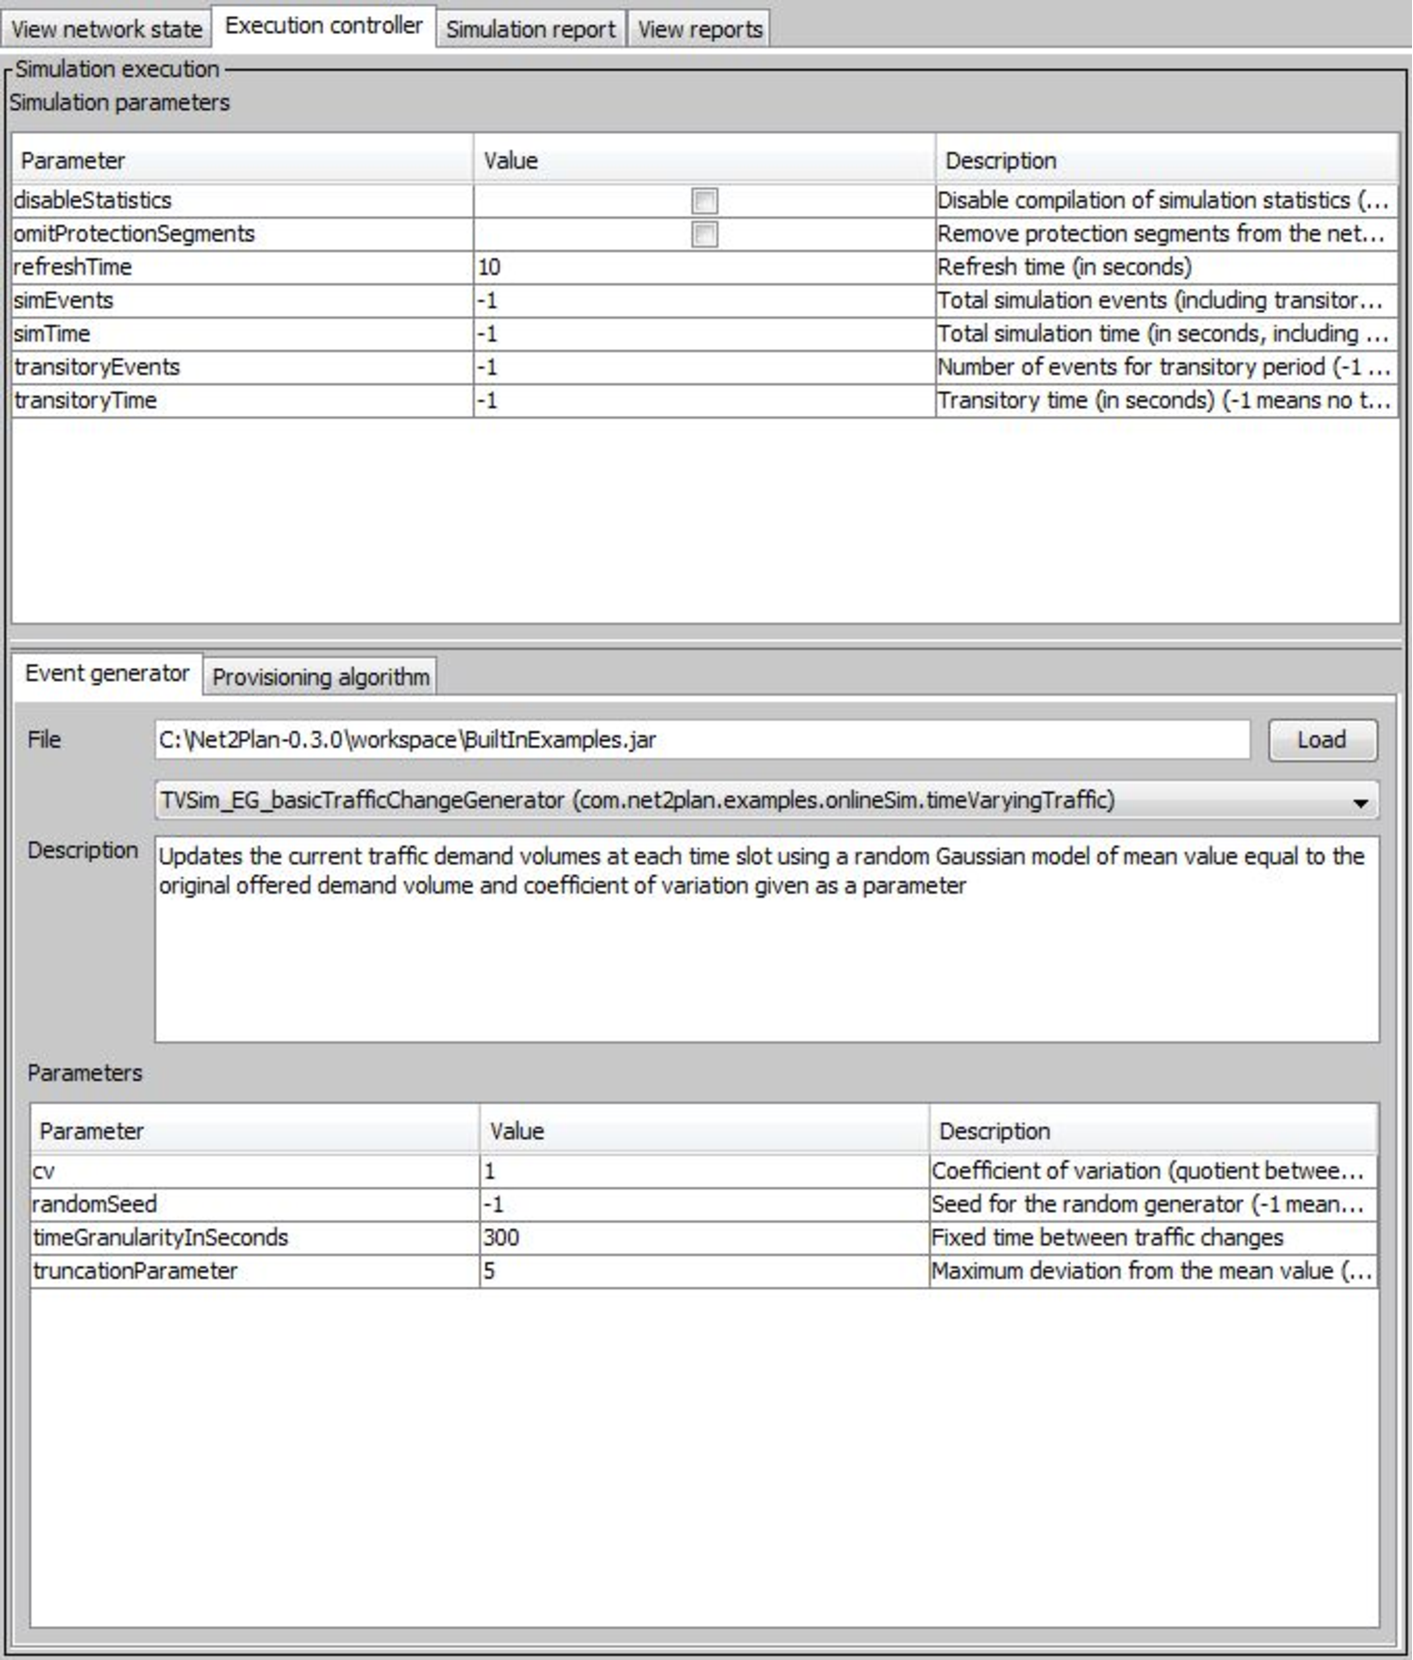
\includegraphics[width = 5cm]{Net2Plan_Simulation.pdf}
			\label{Net2Plan_Simulation}
		}
		\subfigure[]
		{
			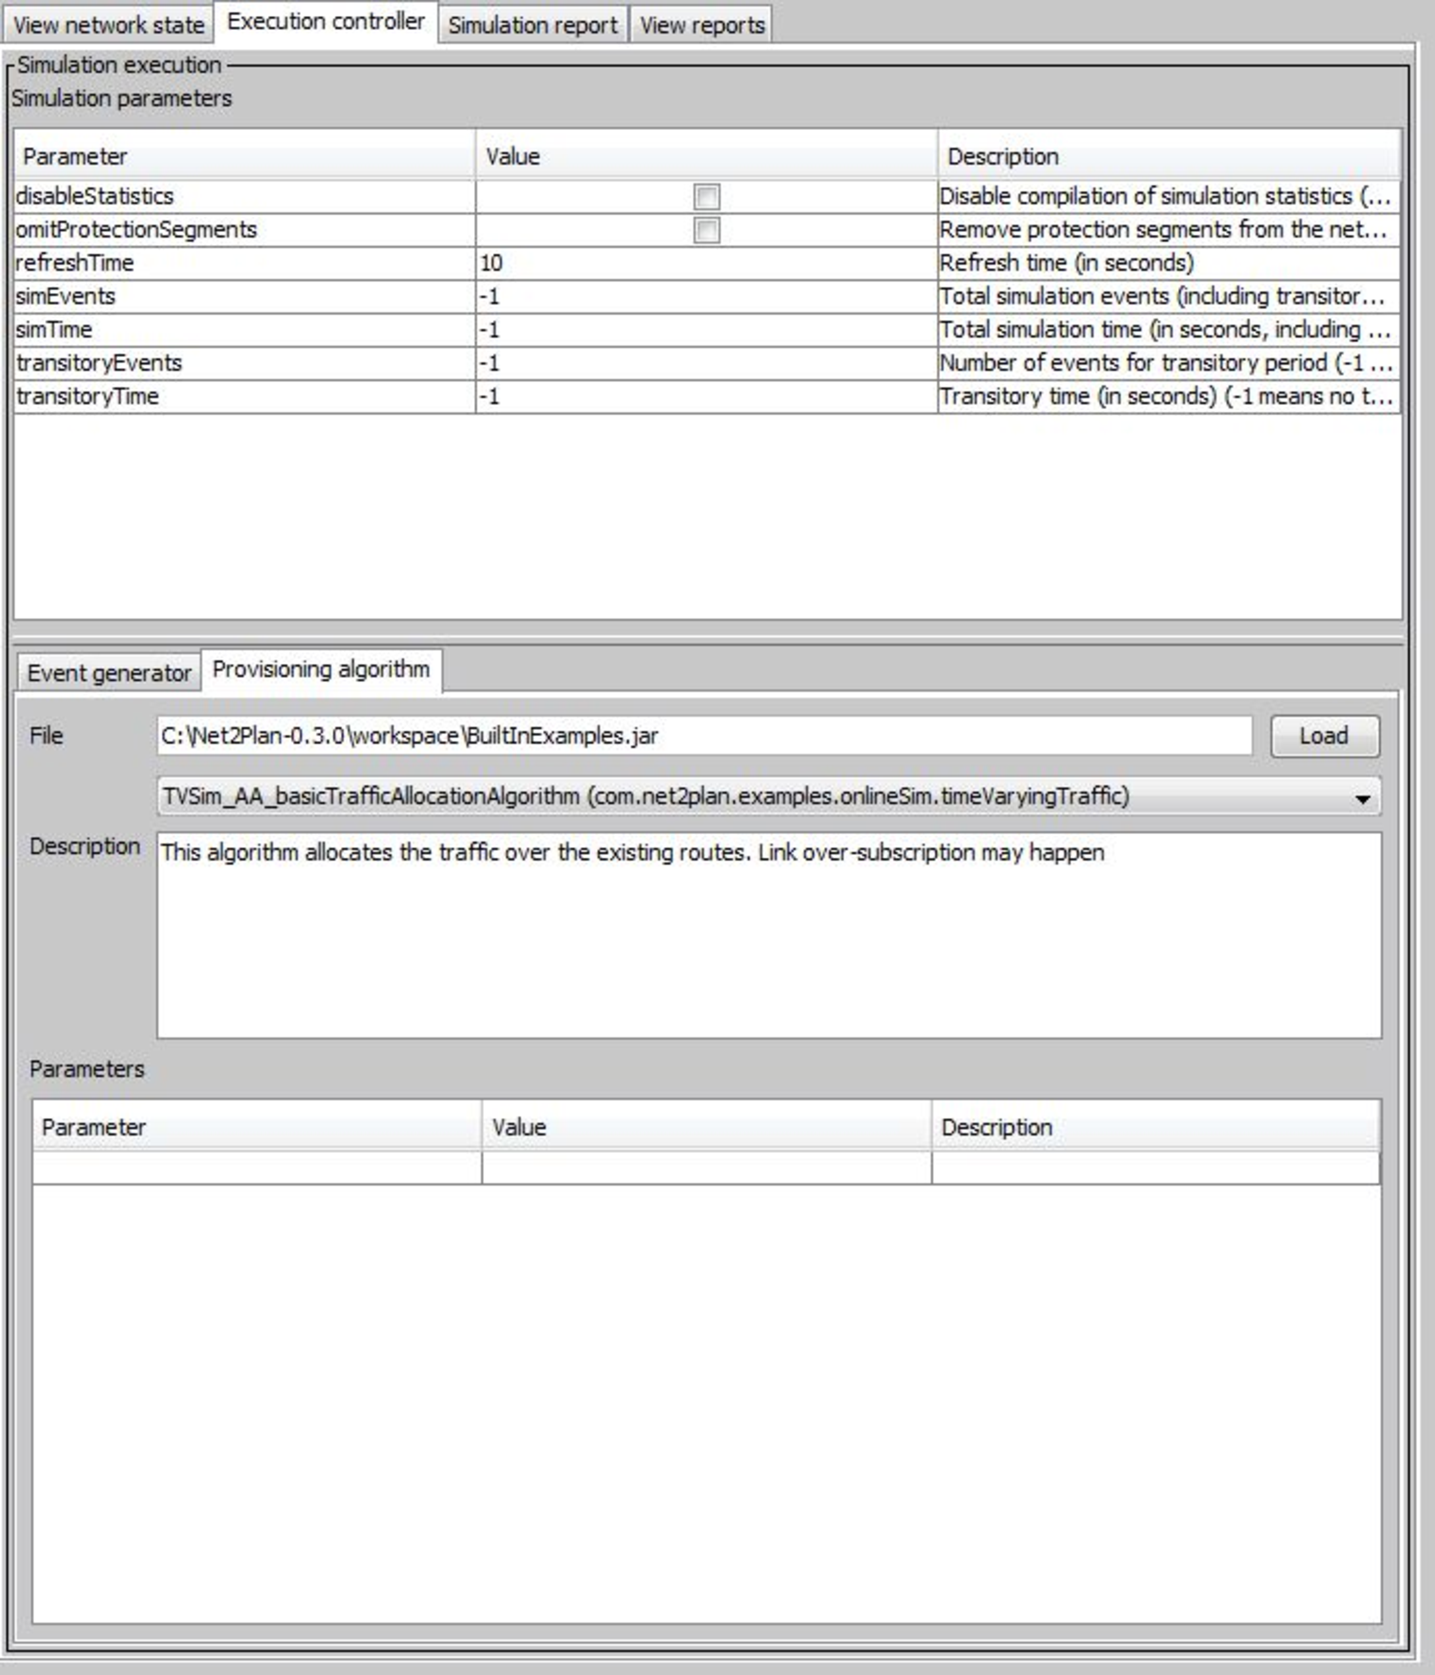
\includegraphics[width = 5cm]{Net2Plan_Simulation_1.pdf}
			\label{Net2Plan_Simulation_1}
		}
		\caption{a) Net2Plan Event generator ; b) Net2Plan Provisioning algorithm}
	\end{figure}	

	The Event generator shown creates a time varying simulation by updating the network traffic based on the chosen parameters while the allocation algorithm in this case only allocates this traffic into the available routes. Besides these options it is also possible to change the main simulation parameters which are displayed on the top half.

	Having defined all the simulation parameters and the other necessary options, the simulation can be started by just pressing "run" below the network topology at the lower left side. The "simulation controller" will update automatically based on the time defined at the simulation parameters or it can be paused for an update on the results.
	
	\newpage

	\section*{Implementing new algorithms on Net2Plan}
	\vspace{1cm}
	This section will demonstrate some of the possibilities provided by Net2Plan as an open source tool. By creating new algorithms or reports it is possible to adapt this program for most necessities in terms of network planning.

	There are already several built-in algorithms present in Net2Plan but as it is impossible to have an algorithm built for every specific necessity it is possible for each user to build new ones or modify existing ones to fulfil what needs to be done.\\
	
	As everything in Net2Plan was built in Java, the program "Eclipse" that can be downloaded from \url{https://eclipse.org/downloads/} was chosen as the best option for coding. All the .java files from the available algorithms in Net2Plan can be downloaded from its website and introduced into "Eclipse" to create a class.
	
	When opening Eclipse, the first choice is to define the work directory in which all the projects will be created. Having defined the workspace, Figure \ref{Eclipse_project} demonstrates the window for creating new projects in Eclipse, this can be accessed by going into "File $\rightarrow$ New $\rightarrow$ Java Project". In this window, only the name needs to be defined and then finish.
	
	\vspace{1.5cm}
	\begin{figure}[h!]
		\centering
		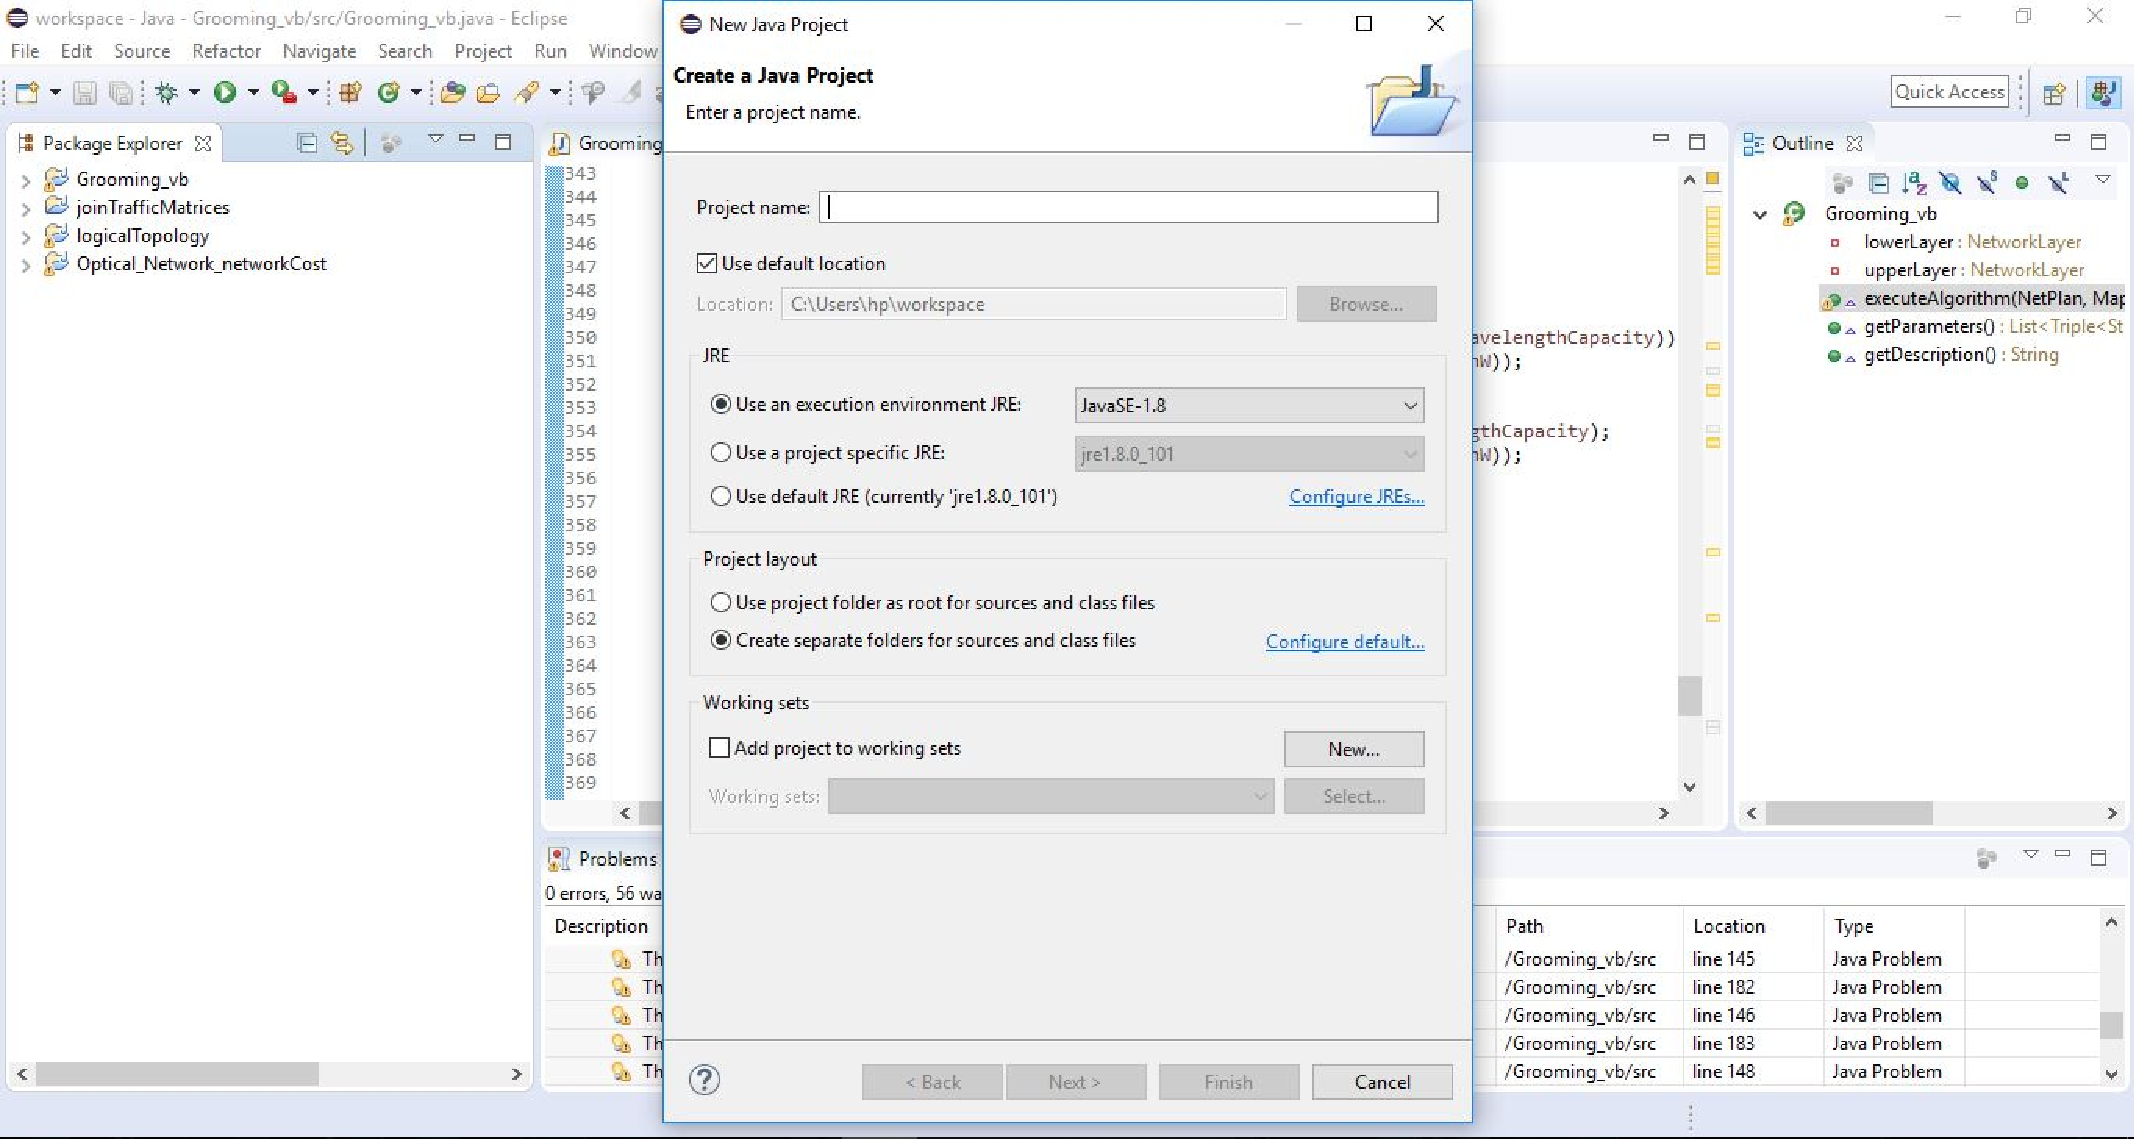
\includegraphics[width = 13cm]{Eclipse_project.pdf}
		\caption{Eclipse new project}
		\label{Eclipse_project}
	\end{figure}	
	
	\newpage
	
	Having created a new project, a "src" directory should be available where the .java should be located. As a starting point, an existing algorithm should be used as a template and then modified to do its necessary purpose. Figure \ref{Eclipse_project_1} shows a newly created project called "logicalTopology".
	
	\vspace{1.5cm}
	\begin{figure}[h!]
		\centering
		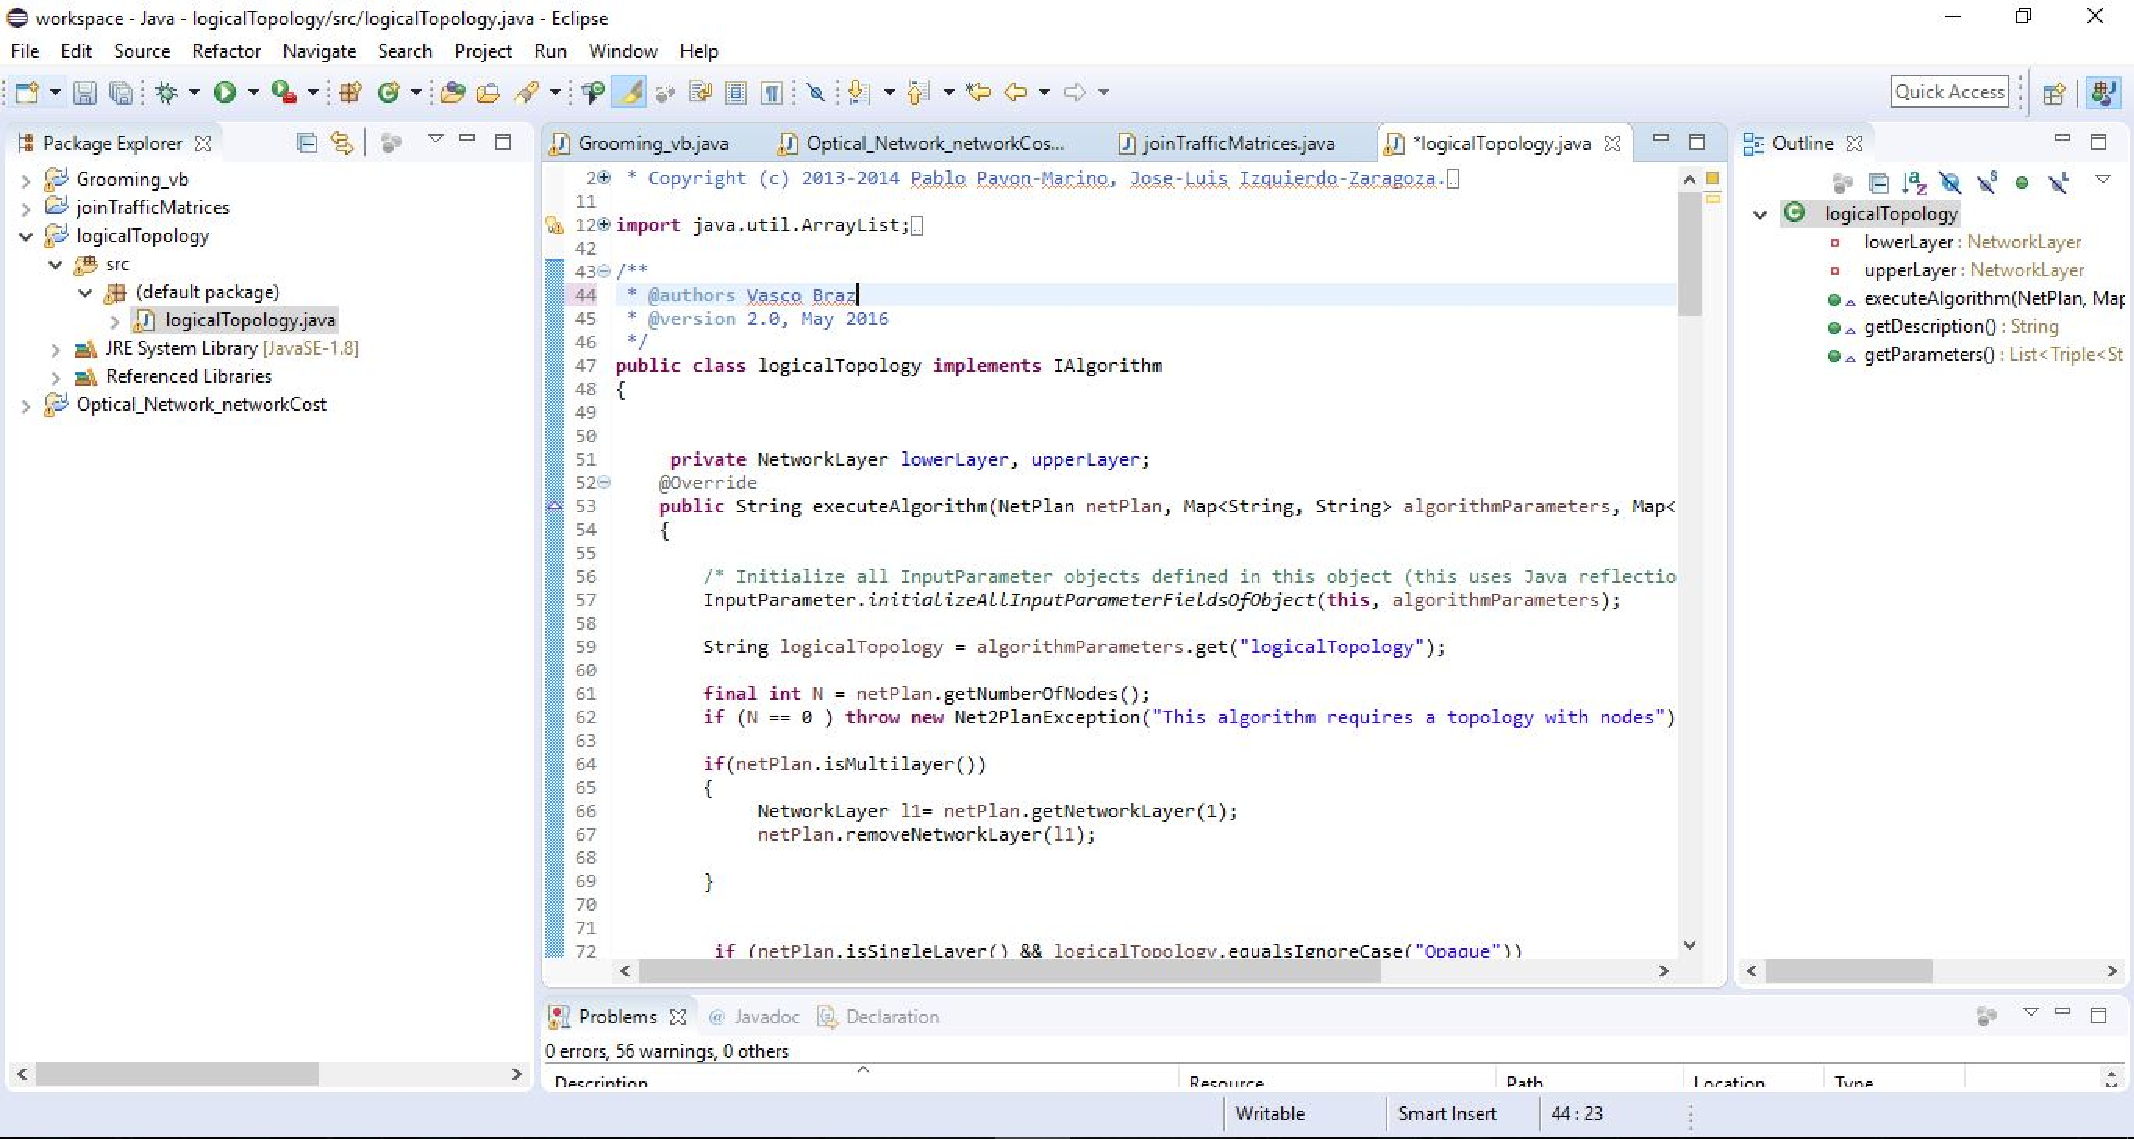
\includegraphics[width = 13cm]{Eclipse_project_1.pdf}
		\caption{Eclipse new project with source file}
		\label{Eclipse_project_1}
	\end{figure}	
	
	To add the library files to a project, right click on it and choose "Build Path $\rightarrow$ Configure Build Path ..." . On the window that appears, press "Add External Jars..." and include all the files in the Net2Plan "lib" directory as shown on Figures \ref{Eclipse_libraries} and \ref{Eclipse_libraries_1}.
	
	\vspace{1.5cm}
	\begin{figure}[!h]
		\centering
		\subfigure[]
		{
			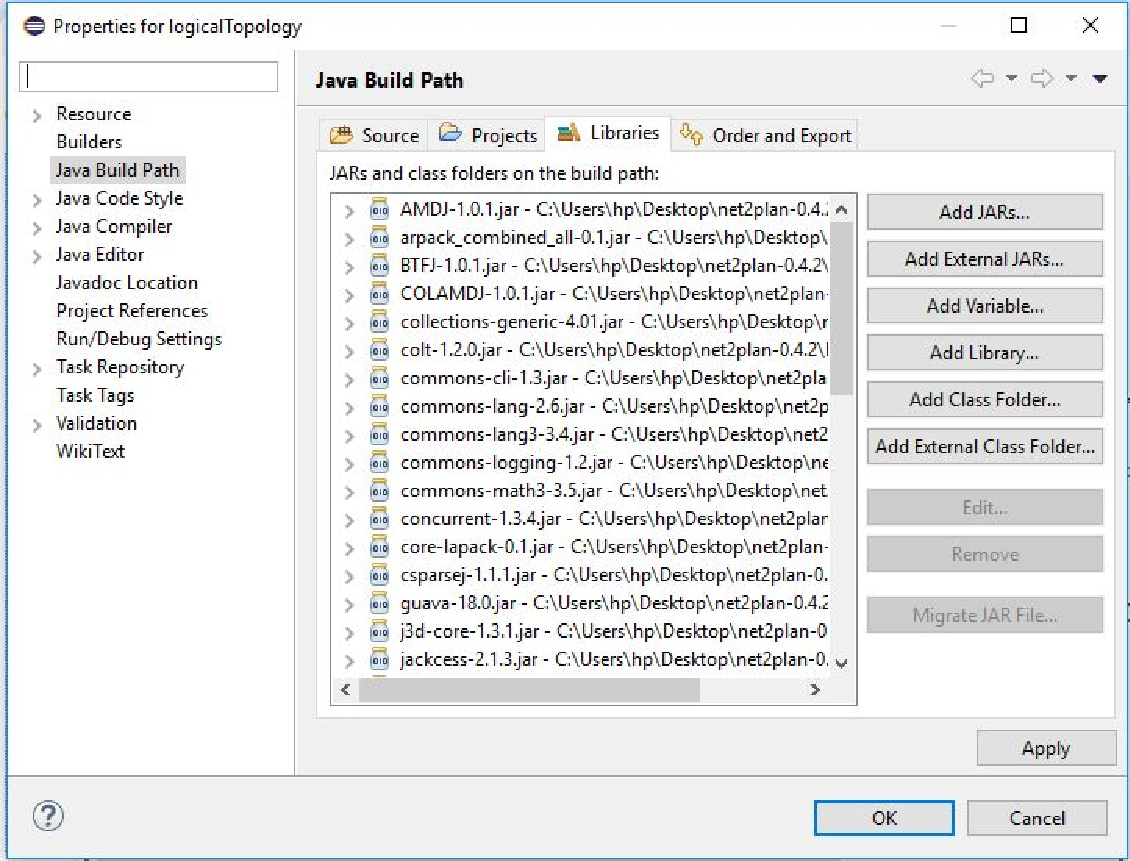
\includegraphics[width = 7.2cm]{Eclipse_libraries.pdf}
			\label{Eclipse_libraries}
		}
		\subfigure[]
		{
			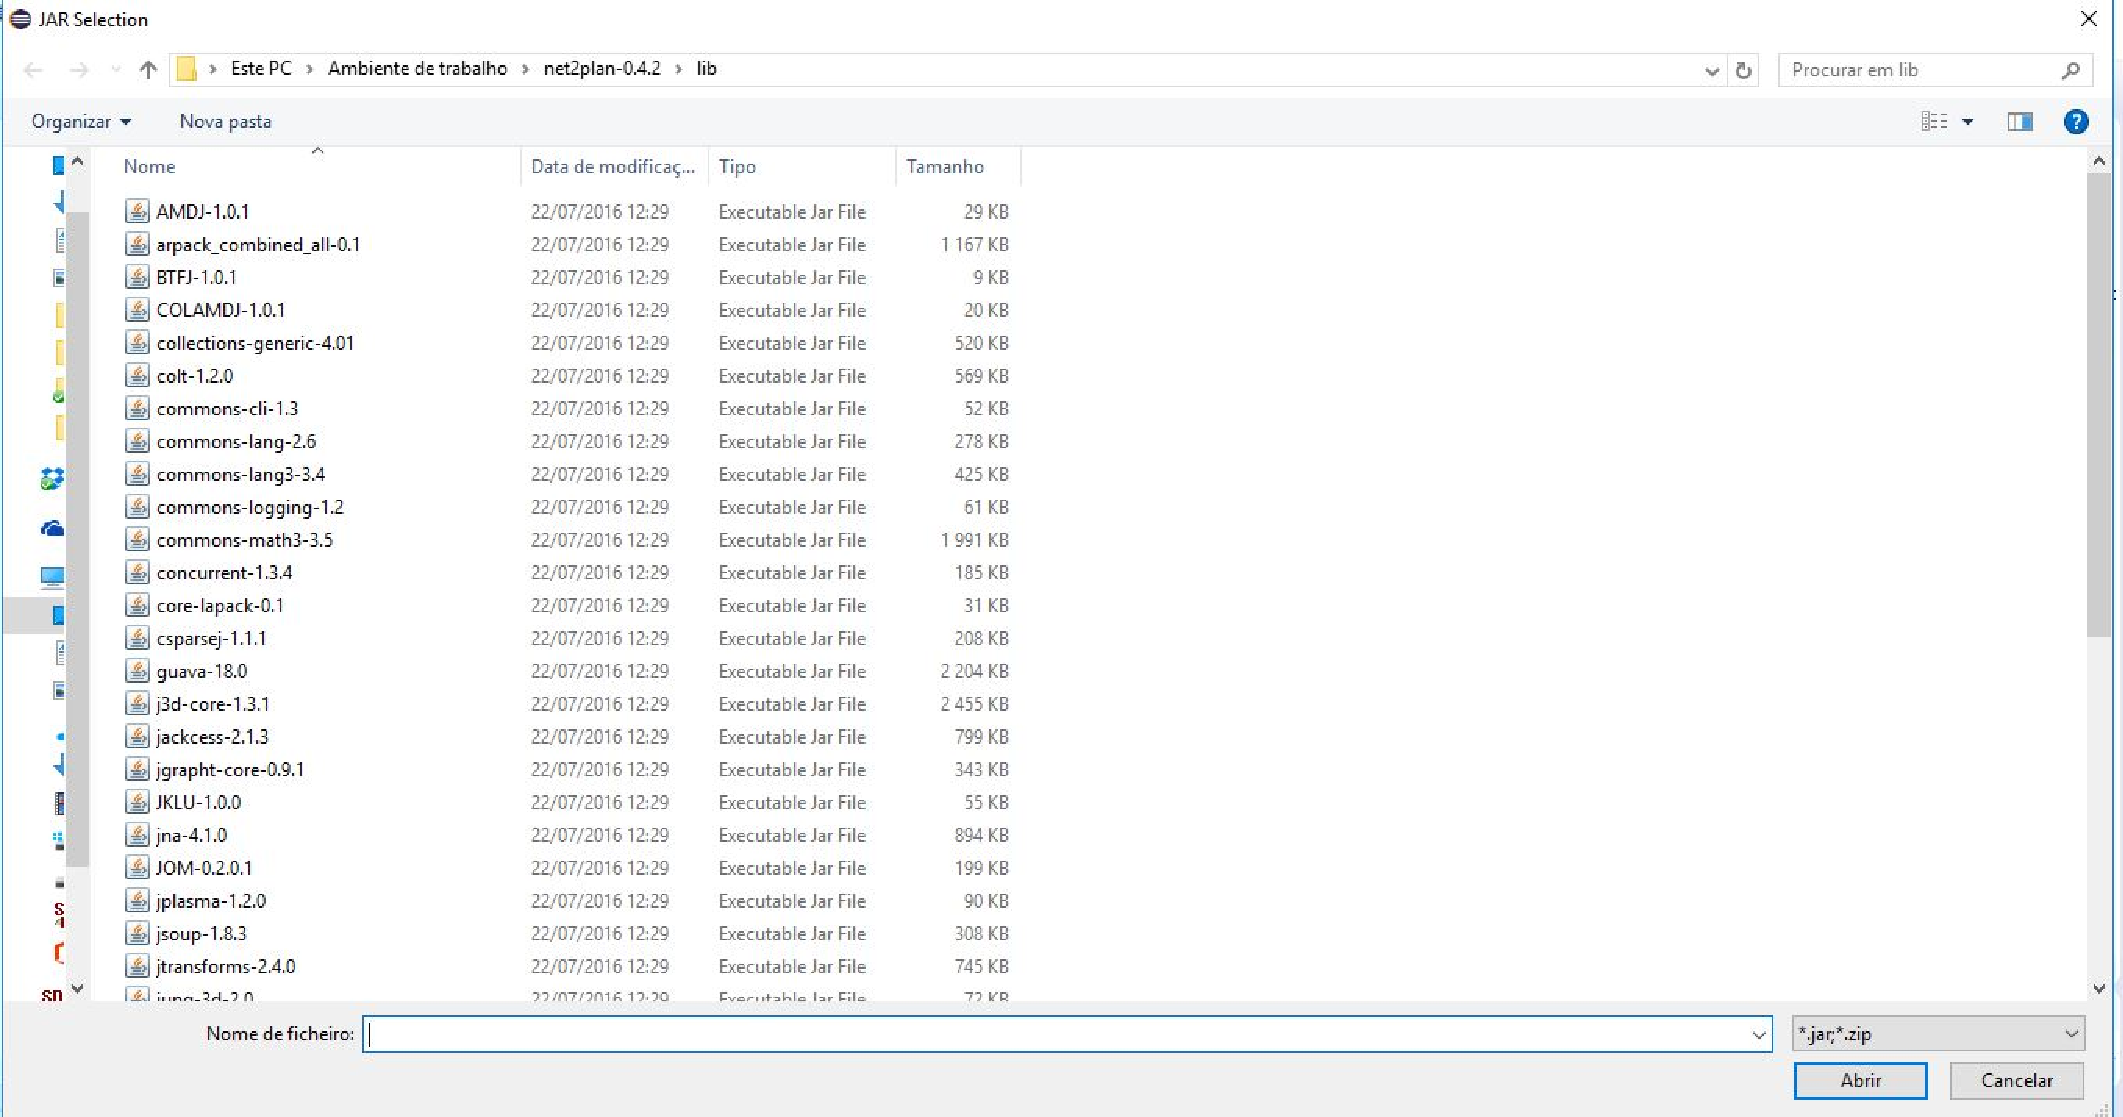
\includegraphics[width = 8.2cm]{Eclipse_libraries_1.pdf}
			\label{Eclipse_libraries_1}
		}
		\caption{a) Eclipse Java Configure Build Path ; b) Net2Plan library files}
	\end{figure}	
	

	
	To further illustrate how these modifications to algorithms work, the project created above using an existing code as a template was modified to create a new algorithm which creates the logical topology of a network in another layer.
	\newpage
	 The code created is shown on Figure \ref{Eclipse_project}.
	By saving this project on Eclipse a .class file is created on the bin directory of the project which can be loaded on Net2Plan. On the "Algorithm execution" tab at the "Offline network design", the "BuiltInExamples.jar" is loaded as the default location for algorithms and as it is a .jar file all the available ones that came with Net2Plan are integrated into it.	To get the newly created algorithm available, press "Load" and find the .class file created in Eclipse as shown on Figure \ref{Net2Plan_introduce_algorithm}.
	
	\begin{figure}[h!]
		\centering
		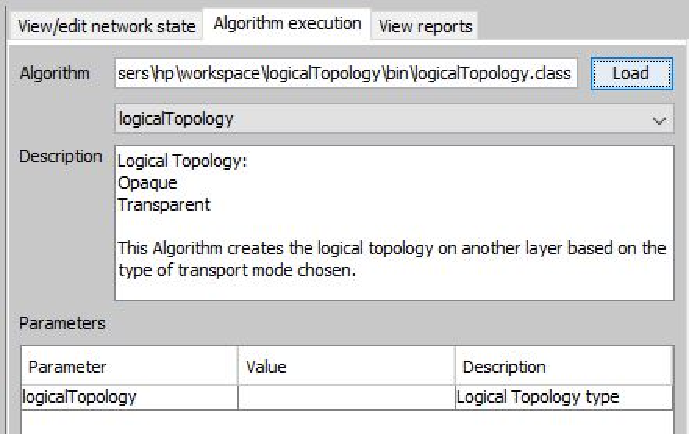
\includegraphics[width = 10.5cm]{Net2Plan_introduce_algorithm.pdf}
		\caption{Net2Plan new algorithm}
		\label{Net2Plan_introduce_algorithm}
	\end{figure}
			
				
			
	As was said before and can be seen on the "Description", this algorithm creates the network logical topology as was explained on section \ref{Creating the Network topologies}.
			
	Algorithms developed on Eclipse can be exported into a .jar file so on Net2Plan this file can be loaded and all the algorithms developed are shown in a list in the same manner as the ones that came with the Net2Plan installation. The export option can be accessed by going into File $\rightarrow$ Export, and the menu are shown in Figures \ref{Eclipse_export} and \ref{Eclipse_export_1}.
	
	\begin{figure}[!h]
		\centering
		\subfigure[]
		{
			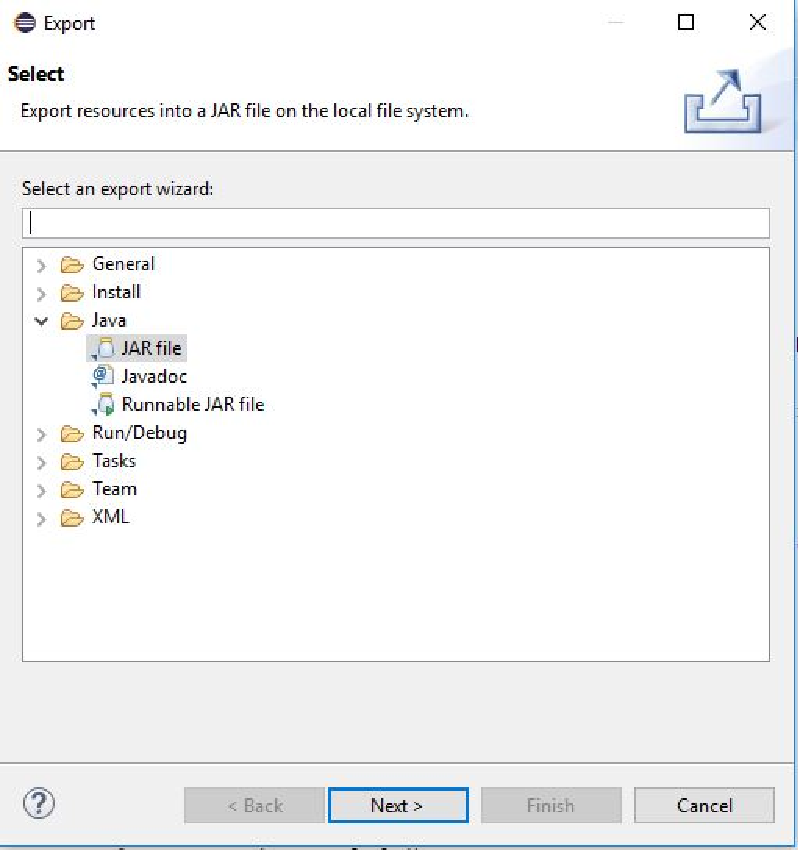
\includegraphics[width = 6cm]{Eclipse_export.pdf}
			\label{Eclipse_export}
		}
		\subfigure[]
		{
			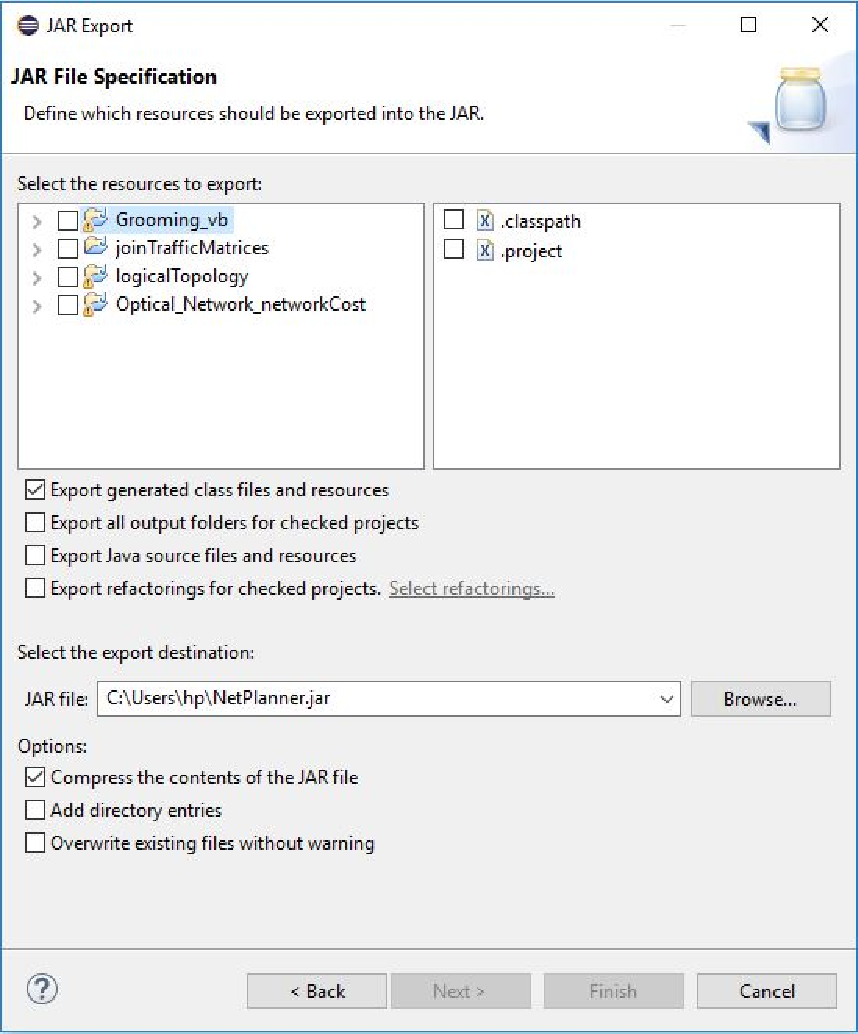
\includegraphics[width = 6cm]{Eclipse_export_1.pdf}
			\label{Eclipse_export_1}
		}
		\caption{a) Eclipse export ; b) Projects to export into a .jar file}
	\end{figure}
	
	By default only the .class files are exported along with the necessary libraries so that the algorithms can be loaded on Net2Plan. There is however an option to also export the .java files so that if needed the ones who will use the code also have access to it if they need to change it.
	 						
	\newpage

	\section*{Developing new Reports}
	Similarly to the way algorithms can be modified or new ones created, also reports can be done using almost the same steps. For the following examples, the "Optical\_Network\_networkcost" is being used as a basis for modifying or creating new reports.

	An important point to note as the main difference as to when modifying algorithms, is that in this case not only are the Net2Plan libraries needed but also the extra files summoned by the report. These files can be found opening the "BuiltInExamples.jar" file in the Net2Plan directory on the corresponding report.

	For the report being used there is an .html file called "main" which is where the information to be displayed in html form is described as well as several image files that are displayed in the report. As such, if the modifications to be done in the reports are to be shown in html format the "main.html" file needs to be modified in order to adapt to these changes.
	
	The tables themselves are created in eclipse as Java code but the html file needs to be opened for example with "Notepadd++" to change some its code as the tables are being appended into the html. Figure \ref{html_report} shows the modified html that is used in the Optical\_Network\_networkcost.
	
	\begin{figure}[h!]
		\centering
		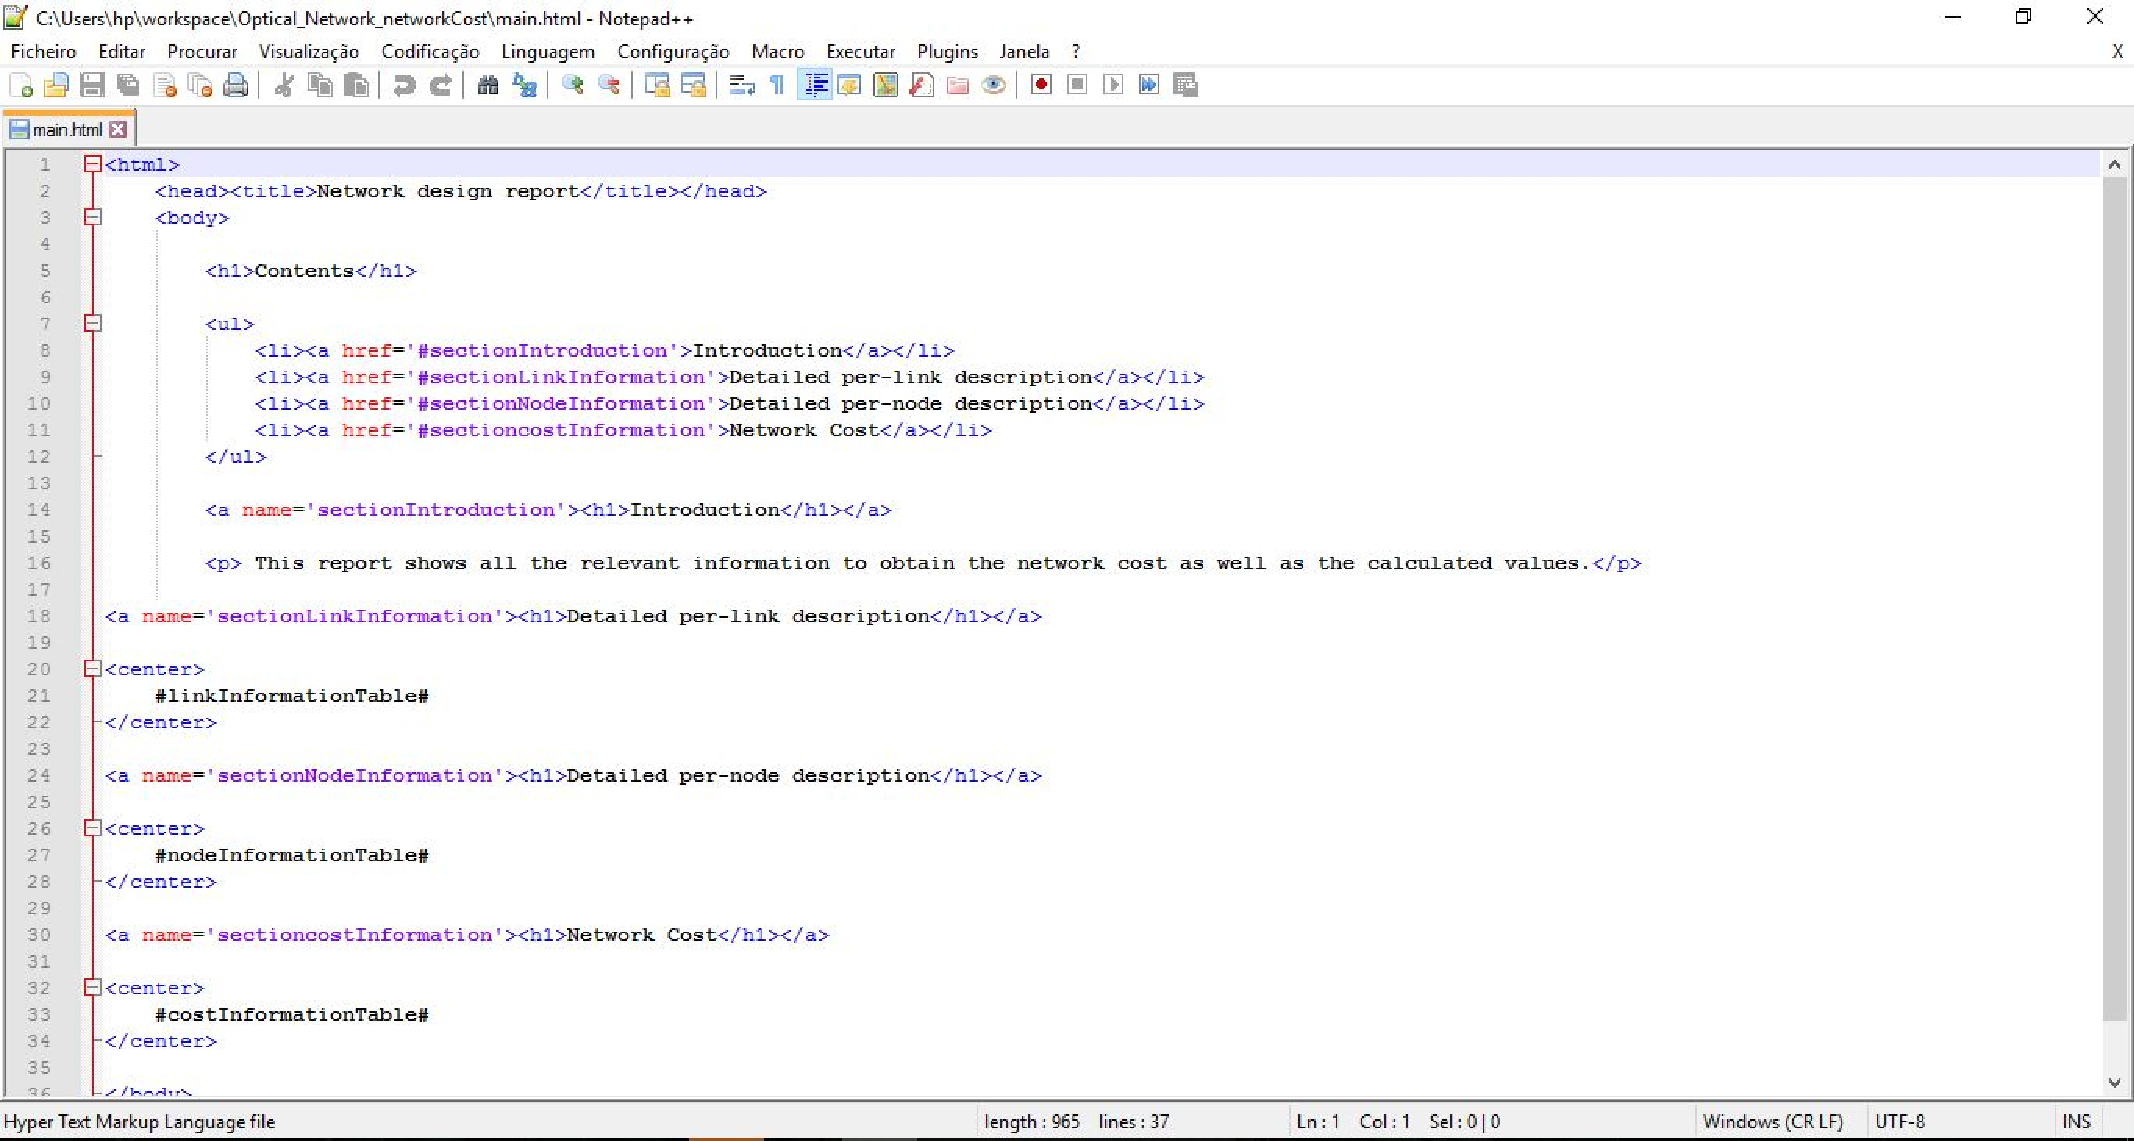
\includegraphics[width = 17cm]{html_report.pdf}
		\caption{html file for Network Cost report}
		\label{html_report}
	\end{figure}	
		
	As can be seen, this is a simple example of an html file since there are only hyper links created to link the contents index to the tables. Other options could be added as for example, hyper links to each of the network costs with the formula describing its calculations by adding the necessary information in this file. These extra options are present on more complex reports such as the "Report\_networkDesign" where the images used are equations showcasing how some of the calculations are done.
	
\clearpage

\clearpage

\section{Installing LPSOLVE for using in MatLab}
\begin{tcolorbox}	
\begin{tabular}{p{2.75cm} p{0.2cm} p{10.5cm}} 	
\textbf{Student Name}  &:& Tiago Esteves        (November 28, 2017 - )\\
\textbf{Goal}          &:& Help other to install lpsolve for using in MatLab.
\end{tabular}
\end{tcolorbox}


In this section will describe how to install lpsolve and how it can be used through matlab. For this it is necessary to follow the following steps:
\begin{enumerate}
  \item Install lpsolve in your computer
  \item Install lpsolve matlab extensions
  \item Install the library
\end{enumerate}

\textbf{Step 1:}\\
The first thing to do is to install lpsolve using the execute file "lp-solve-5.5.2.5-IDE-Setup" that can be found in GitHub through this link \url{https://github.com/netxpto/NetPlanner/tree/Develop/software/lpsolve}. The installation is quite simple and contains few steps for its execution. \\
In case there is any doubt or question you can always use the lpsolve reference guide in link: \url{http://lpsolve.sourceforge.net/5.5/} \\

\textbf{Step 2:}\\
In this step it is necessary to go to GitHub again and download with the name "lp-solve-5.5.2.0-MATLAB-exe-win64" in link \url{https://github.com/netxpto/NetPlanner/tree/Develop/software/lpsolve} and extract all the files. Then you need to put the \textbf{mxlpsolve.mexw64} and \textbf{mxlpsolve.m} files in the same folder as the .m files. \\
In case there is any doubt or question you can always use this guide for help: \url{there is any doubt or question you can always use the lpsolve reference guide in link:} \\

\textbf{Setp 3:}\\
Finally, once again in GitHub through the link \url{https://github.com/netxpto/NetPlanner/tree/Develop/software/lpsolve} we can find the last folder to get the necessary library, thus downloading the folder "lp-solve-5.5.2.0-dev-win64" and then include in the Windows PATH environment. \\


\clearpage

\section{Opaque with 1+1 protection appendices}
\begin{tcolorbox}	
\begin{tabular}{p{2.75cm} p{0.2cm} p{10.5cm}} 	
\textbf{Student Name}  &:& Tiago Esteves    (November 28, 2017 - )\\
\textbf{Goal}          &:& Implement the dimensioning of optical networks in the opaque transport mode.
\end{tabular}
\end{tcolorbox}


\subsection{Script using MatLab}

\subsubsection{Scenario 1}

\qquad RESULTS: Test Network \\

\quad Scenario: Opaque Low Traffic \\

Number of optical channels in the link (1,2): 2 \\
\qquad Number of optical channels in the link (1,3): 2 \\
\qquad Number of optical channels in the link (2,3): 4 \\
\qquad Number of optical channels in the link (2,4): 3 \\
\qquad Number of optical channels in the link (3,5): 3 \\
\qquad Number of optical channels in the link (4,5): 3 \\
\qquad Number of optical channels in the link (4,6): 3 \\
\qquad Number of optical channels in the link (5,6): 3 \\

---------------Demand (1,2)--------------- \\

------Working Path------ \\
Link  (1,2) \\
Number of links: 1 \\

-----Protection Path----- \\
Link  (1,3) \\
Link  (3,2) \\
Number of links: 2 \\

---------------Demand (1,3)--------------- \\

------Working Path------ \\
Link  (1,3) \\
Number of links: 1 \\

-----Protection Path----- \\
Link  (1,2) \\
Link  (2,3) \\
Number of links: 2 \\

---------------Demand (2,3)--------------- \\

------Working Path------ \\
Link  (2,3) \\
Number of links: 1 \\

-----Protection Path----- \\
Link  (2,1) \\
Link  (1,3) \\
Number of links: 2 \\

---------------Demand (2,4)--------------- \\

------Working Path------ \\
Link  (2,4) \\
Number of links: 1 \\

-----Protection Path----- \\
Link  (2,3) \\
Link  (3,5) \\
Link  (5,4) \\
Number of links: 3 \\

---------------Demand (3,5)--------------- \\

------Working Path------ \\
Link  (3,5) \\
Number of links: 1 \\

-----Protection Path----- \\
Link  (3,2) \\
Link  (2,4) \\
Link  (4,5) \\
Number of links: 3 \\

---------------Demand (4,5)--------------- \\

------Working Path------ \\
Link  (4,5) \\
Number of links: 1 \\

-----Protection Path----- \\
Link  (4,6) \\
Link  (6,5) \\
Number of links: 2 \\

---------------Demand (4,6)--------------- \\

------Working Path------ \\
Link  (4,6) \\
Number of links: 1 \\

-----Protection Path----- \\
Link  (4,5) \\
Link  (5,6) \\
Number of links: 2 \\

---------------Demand (5,6)--------------- \\

------Working Path------ \\
Link  (5,6) \\
Number of links: 1 \\

-----Protection Path----- \\
Link  (5,4) \\
Link  (4,6) \\
Number of links: 2 \\

\subsubsection{Scenario 2}

\qquad RESULTS: Test Network \\

\quad Scenario: Opaque High Traffic \\

Number of optical channels in the link (1,2): 12 \\
\qquad Number of optical channels in the link (1,3): 12 \\
\qquad Number of optical channels in the link (2,3): 33 \\
\qquad Number of optical channels in the link (2,4): 28 \\
\qquad Number of optical channels in the link (3,5): 28 \\
\qquad Number of optical channels in the link (4,5): 26 \\
\qquad Number of optical channels in the link (4,6): 30 \\
\qquad Number of optical channels in the link (5,6): 30 \\


---------------Demand (1,2)--------------- \\

------Working Path------ \\
Link  (1,2) \\
Number of links: 1 \\

-----Protection Path----- \\
Link  (1,3) \\
Link  (3,2) \\
Number of links: 2 \\


---------------Demand (1,3)--------------- \\

------Working Path------ \\
Link  (1,3) \\
Number of links: 1 \\

-----Protection Path----- \\
Link  (1,2) \\
Link  (2,3) \\
Number of links: 2 \\


---------------Demand (2,3)--------------- \\

------Working Path------ \\
Link  (2,3) \\
Number of links: 1 \\

-----Protection Path----- \\
Link  (2,1) \\
Link  (1,3) \\
Number of links: 2 \\


---------------Demand (2,4)--------------- \\

------Working Path------ \\
Link  (2,4) \\
Number of links: 1 \\

-----Protection Path----- \\
Link  (2,3) \\
Link  (3,5) \\
Link  (5,4) \\
Number of links: 3 \\


---------------Demand (3,5)--------------- \\

------Working Path------ \\
Link  (3,5) \\
Number of links: 1 \\

-----Protection Path----- \\
Link  (3,2) \\
Link  (2,4) \\
Link  (4,5) \\
Number of links: 3 \\


---------------Demand (4,5)--------------- \\

------Working Path------ \\
Link  (4,5) \\
Number of links: 1 \\

-----Protection Path----- \\
Link  (4,6) \\
Link  (6,5) \\
Number of links: 2 \\


---------------Demand (4,6)--------------- \\

------Working Path------ \\
Link  (4,6) \\
Number of links: 1 \\

-----Protection Path----- \\
Link  (4,5) \\
Link  (5,6) \\
Number of links: 2 \\


---------------Demand (5,6)--------------- \\

------Working Path------ \\
Link  (5,6) \\
Number of links: 1 \\

-----Protection Path----- \\
Link  (5,4) \\
Link  (4,6) \\
Number of links: 2 \\

\subsubsection{Scenario 3}

\subsubsection{Scenario 4}


\subsection{ILP using LPSolve}

\subsubsection{Scenario 1}

/* Objective function */ \\
min: +C1 +C2 +C3 +C4 +C5 +C6 +C7 +C8 +C9 +C10 +C11 +C12 +C13 +C14 +C15 +C16 +C17 +C18 +C19 +C20 +C21 +C22
 +C23 +C24 +C25 +C26 +C27 +C28 +C29 +C30 +C31 +C32 +C33 +C34 +C35 +C36 +C37 +C38 +C39 +C40 +C41 +C42
 +C43 +C44 +C45 +C46 +C47 +C48 +C49 +C50 +C51 +C52 +C53 +C54 +C55 +C56 +C57 +C58 +C59 +C60 +C61 +C62
 +C63 +C64 +C65 +C66 +C67 +C68 +C69 +C70 +C71 +C72 +C73 +C74 +C75 +C76 +C77 +C78 +C79 +C80 +C81 +C82
 +C83 +C84 +C85 +C86 +C87 +C88 +C89 +C90 +C91 +C92 +C93 +C94 +C95 +C96 +C97 +C98 +C99 +C100 +C101 +C102
 +C103 +C104 +C105 +C106 +C107 +C108 +C109 +C110 +C111 +C112 +C113 +C114 +C115 +C116 +C117 +C118 +C119
 +C120 +C121 +C122 +C123 +C124 +C125 +C126 +C127 +C128 +C129 +C130 +C131 +C132 +C133 +C134 +C135 +C136
 +C137 +C138 +C139 +C140 +C141 +C142 +C143 +C144 +C145 +C146 +C147 +C148 +C149 +C150 +C151 +C152 +C153
 +C154 +C155 +C156 +C157 +C158 +C159 +C160 +C161 +C162 +C163 +C164 +C165 +C166 +C167 +C168 +C169 +C170
 +C171 +C172 +C173 +C174 +C175 +C176 +C177 +C178 +C179 +C180 +C181 +C182 +C183 +C184 +C185 +C186 +C187
 +C188 +C189 +C190 +C191 +C192 +C193 +C194 +C195 +C196 +C197 +C198 +C199 +C200 +C201 +C202 +C203 +C204
 +C205 +C206 +C207 +C208 +C209 +C210 +C211 +C212 +C213 +C214 +C215 +C216 +C217 +C218 +C219 +C220 +C221
 +C222 +C223 +C224 +C225 +C226 +C227 +C228 +C229 +C230 +C231 +C232 +C233 +C234 +C235 +C236 +C237 +C238
 +C239 +C240 +C241 +C242 +C243 +C244 +C245 +C246 +C247 +C248 +C249 +C250 +C251 +C252 +C253 +C254 +C255
 +C256 +C257 +C258 +C259 +C260 +C261 +C262 +C263 +C264 +C265 +C266 +C267 +C268 +C269 +C270 +C271 +C272
 +C273 +C274 +C275 +C276 +C277 +C278 +C279 +C280 +C281 +C282 +C283 +C284 +C285 +C286 +C287 +C288 +C289
 +C290 +C291 +C292 +C293 +C294 +C295 +C296 +C297 +C298 +C299 +C300 +C301 +C302 +C303 +C304 +C305 +C306
 +C307 +C308 +C309 +C310 +C311 +C312 +C313 +C314 +C315 +C316 +C317 +C318 +C319 +C320 +C321 +C322 +C323
 +C324 +C325 +C326 +C327 +C328 +C329 +C330 +C331 +C332 +C333 +C334 +C335 +C336 +C337 +C338 +C339 +C340
 +C341 +C342 +C343 +C344 +C345 +C346 +C347 +C348 +C349 +C350 +C351 +C352 +C353 +C354 +C355 +C356 +C357
 +C358 +C359 +C360 +C361 +C362 +C363 +C364 +C365 +C366 +C367 +C368 +C369 +C370 +C371 +C372 +C373 +C374
 +C375 +C376 +C377 +C378 +C379 +C380 +C381 +C382 +C383 +C384 +C385 +C386 +C387 +C388 +C389 +C390 +C391
 +C392 +C393 +C394 +C395 +C396 +C397 +C398 +C399 +C400 +C401 +C402 +C403 +C404 +C405 +C406 +C407 +C408
 +C409 +C410 +C411 +C412 +C413 +C414 +C415 +C416 +C417 +C418 +C419 +C420 +C421 +C422 +C423 +C424 +C425
 +C426 +C427 +C428 +C429 +C430 +C431 +C432 +C433 +C434 +C435 +C436 +C437 +C438 +C439 +C440 +C441 +C442
 +C443 +C444 +C445 +C446 +C447 +C448 +C449 +C450 +C451 +C452 +C453 +C454 +C455 +C456 +C457 +C458 +C459
 +C460 +C461 +C462 +C463 +C464 +C465 +C466 +C467 +C468 +C469 +C470 +C471 +C472 +C473 +C474 +C475 +C476
 +C477 +C478 +C479 +C480 +C481 +C482 +C483 +C484 +C485 +C486 +C487 +C488 +C489 +C490 +C491 +C492 +C493
 +C494 +C495 +C496 +C497 +C498 +C499 +C500 +C501 +C502 +C503 +C504 +C505 +C506 +C507 +C508 +C509 +C510
 +C511 +C512 +C513 +C514 +C515 +C516 +C517 +C518 +C519 +C520 +C521 +C522 +C523 +C524 +C525 +C526 +C527
 +C528 +C529 +C530 +C531 +C532 +C533 +C534 +C535 +C536 +C537 +C538 +C539 +C540 +C541 +C542 +C543 +C544
 +C545 +C546 +C547 +C548 +C549 +C550 +C551 +C552 +C553 +C554 +C555 +C556 +C557 +C558 +C559 +C560 +C561
 +C562 +C563 +C564 +C565 +C566 +C567 +C568 +C569 +C570 +C571 +C572 +C573 +C574 +C575 +C576 +C577 +C578
 +C579 +C580 +C581 +C582 +C583 +C584 +C585 +C586 +C587 +C588 +C589 +C590 +C591 +C592 +C593 +C594 +C595
 +C596 +C597 +C598 +C599 +C600 +C601 +C602 +C603 +C604 +C605 +C606 +C607 +C608 +C609 +C610 +C611 +C612
 +C613 +C614 +C615 +C616 +C617 +C618 +C619 +C620 +C621 +C622 +C623 +C624 +C625 +C626 +C627 +C628 +C629
 +C630 +C631 +C632 +C633 +C634 +C635 +C636 +C637 +C638 +C639 +C640 +C641 +C642 +C643 +C644 +C645 +C646
 +C647 +C648 +C649 +C650 +C651 +C652 +C653 +C654 +C655 +C656 +C657 +C658 +C659 +C660 +C661 +C662 +C663
 +C664 +C665 +C666 +C667 +C668 +C669 +C670 +C671 +C672 +C673 +C674 +C675 +C676 +C677 +C678 +C679 +C680
 +C681 +C682 +C683 +C684 +C685 +C686 +C687 +C688 +C689 +C690 +C691 +C692 +C693 +C694 +C695 +C696 +C697
 +C698 +C699 +C700 +C701 +C702 +C703 +C704 +C705 +C706 +C707 +C708 +C709 +C710 +C711 +C712 +C713 +C714
 +C715 +C716 +C717 +C718 +C719 +C720 +C721 +C722 +C723 +C724 +C725 +C726 +C727 +C728 +C729 +C730 +C731
 +C732 +C733 +C734 +C735 +C736 +C737 +C738 +C739 +C740 +C741 +C742 +C743 +C744 +C745 +C746 +C747 +C748
 +C749 +C750 +C751 +C752 +C753 +C754 +C755 +C756 +C757 +C758 +C759 +C760 +C761 +C762 +C763 +C764 +C765
 +C766 +C767 +C768 +C769 +C770 +C771 +C772 +C773 +C774 +C775 +C776 +C777 +C778 +C779 +C780 +C781 +C782
 +C783 +C784 +C785 +C786 +C787 +C788 +C789 +C790 +C791 +C792 +C793 +C794 +C795 +C796 +C797 +C798 +C799
 +C800 +C801 +C802 +C803 +C804 +C805 +C806 +C807 +C808 +C809 +C810 +C811 +C812 +C813 +C814 +C815 +C816
 +C817 +C818 +C819 +C820 +C821 +C822 +C823 +C824 +C825 +C826 +C827 +C828 +C829 +C830 +C831 +C832 +C833
 +C834 +C835 +C836 +C837 +C838 +C839 +C840 +C841 +C842 +C843 +C844 +C845 +C846 +C847 +C848 +C849 +C850
 +C851 +C852 +C853 +C854 +C855 +C856 +C857 +C858 +C859 +C860 +C861 +C862 +C863 +C864 +C865 +C866 +C867
 +C868 +C869 +C870 +C871 +C872 +C873 +C874 +C875 +C876 +C877 +C878 +C879 +C880 +C881 +C882 +C883 +C884
 +C885 +C886 +C887 +C888 +C889 +C890 +C891 +C892 +C893 +C894 +C895 +C896 +C897 +C898 +C899 +C900 +C901
 +C902 +C903 +C904 +C905 +C906 +C907 +C908 +C909 +C910 +C911 +C912 +C913 +C914 +C915; \\

/* Constraints */ \\
+C1 +C2 = 2;
+C1 +C12 +C17 = 2;
-C2 +C12 +C14 -C23 = 0;
+C17 +C19 +C20 -C24 -C29 = 0;
-C14 -C19 +C23 +C24 +C25 -C30 = 0;
-C20 -C25 +C29 +C30 = 0;
+C31 +C32 = 2;
-C31 +C37 +C38 -C47 = 0;
+C32 +C37 +C53 = 2;
-C38 +C47 +C49 +C50 -C54 -C59 = 0;
-C49 +C53 +C54 +C55 -C60 = 0;
-C50 -C55 +C59 +C60 = 0;
+C61 +C62 = 2;
-C61 +C67 +C68 -C72 = 0;
-C62 -C67 +C72 +C74 -C83 = 0;
+C68 +C84 +C89 = 2;
-C74 +C83 +C84 +C85 -C90 = 0;
-C85 +C89 +C90 = 0;
+C91 +C92 = 2;
-C91 +C97 +C98 -C102 -C107 = 0;
-C92 -C97 +C102 +C104 = 0;
-C98 +C107 +C109 +C110 -C119 = 0;
+C104 +C109 +C120 = 2;
-C110 +C119 +C120 = 0;
+C121 +C122 = 2;
-C121 +C127 +C128 -C132 -C137 = 0;
-C122 -C127 +C132 +C134 -C143 = 0;
-C128 +C137 +C139 +C140 -C144 = 0;
-C134 -C139 +C143 +C144 +C145 = 0;
+C140 +C145 = 2;
+C152 -C156 = 0;
+C156 +C157 +C158 = 2;
+C152 +C157 +C173 = 2;
-C158 +C169 +C170 -C174 -C179 = 0;
-C169 +C173 +C174 +C175 -C180 = 0;
-C170 -C175 +C179 +C180 = 0;
+C182 -C186 -C191 = 0;
+C186 +C187 +C188 = 2;
-C182 -C187 +C191 +C194 -C203 = 0;
+C188 +C204 +C209 = 2;
-C194 +C203 +C204 +C205 -C210 = 0;
-C205 +C209 +C210 = 0;
+C212 -C216 -C221 = 0;
+C216 +C217 +C218 = 2;
-C212 -C217 +C221 +C224 = 0;
-C218 +C229 +C230 -C239 = 0;
+C224 +C229 +C240 = 2;
-C230 +C239 +C240 = 0;
+C242 -C246 -C251 = 0;
+C246 +C247 +C248 = 2;
-C242 -C247 +C251 +C254 -C263 = 0;
-C248 +C259 +C260 -C264 = 0;
-C254 -C259 +C263 +C264 +C265 = 0;
+C260 +C265 = 2;
+C271 -C276 -C281 = 0;
-C271 +C276 +C278 -C282 = 0;
+C281 +C282 +C284 = 2;
+C278 +C294 +C299 = 2;
-C284 +C294 +C295 -C300 = 0;
-C295 +C299 +C300 = 0;
+C301 -C306 -C311 = 0;
-C301 +C306 +C308 -C312 -C317 = 0;
+C311 +C312 +C314 = 2;
-C308 +C317 +C319 +C320 -C329 = 0;
+C314 +C319 +C330 = 2;
-C320 +C329 +C330 = 0;
+C331 -C336 -C341 = 0;
-C331 +C336 +C338 -C342 -C347 = 0;
+C341 +C342 +C344 = 2;
-C338 +C347 +C349 +C350 -C354 = 0;
-C344 -C349 +C354 +C355 = 0;
+C350 +C355 = 2;
+C361 +C362 -C366 -C371 = 0;
-C361 +C366 +C367 -C372 -C377 = 0;
-C362 -C367 +C371 +C372 +C374 = 0;
+C377 +C379 +C380 = 2;
+C374 +C379 +C390 = 2;
-C380 +C390 = 0;
+C391 +C392 -C396 -C401 = 0;
-C391 +C396 +C397 -C402 -C407 = 0;
-C392 -C397 +C401 +C402 +C404 -C413 = 0;
+C407 +C409 +C410 = 2;
-C404 -C409 +C413 +C415 = 0;
+C410 +C415 = 2;
+C421 +C422 -C426 -C431 = 0;
-C421 +C426 +C427 +C428 -C432 -C437 = 0;
-C422 -C427 +C431 +C432 -C443 = 0;
-C428 +C437 +C440 -C444 = 0;
+C443 +C444 +C445 = 2;
+C440 +C445 = 2;
+21.25 C1 +21.25 C6 +21.25 C31 +21.25 C36 +18.75 C61 +18.75 C66 +1.25 C91 +1.25 C96 +16.25 C121 +16.25 C126
 +40 C151 +40 C156 +8.75 C181 +8.75 C186 +18.75 C211 +18.75 C216 +142.5 C241 +142.5 C246 +13.75 C271
 +13.75 C276 +57.5 C301 +57.5 C306 +1.25 C331 +1.25 C336 +13.75 C361 +13.75 C366 +8.75 C391 +8.75 C396
 +116.25 C421 +116.25 C426 -100 C901 <= 0;
+21.25 C2 +21.25 C11 +21.25 C32 +21.25 C41 +18.75 C62 +18.75 C71 +1.25 C92 +1.25 C101 +16.25 C122 +16.25 C131
 +40 C152 +40 C161 +8.75 C182 +8.75 C191 +18.75 C212 +18.75 C221 +142.5 C242 +142.5 C251 +13.75 C272
 +13.75 C281 +57.5 C302 +57.5 C311 +1.25 C332 +1.25 C341 +13.75 C362 +13.75 C371 +8.75 C392 +8.75 C401
 +116.25 C422 +116.25 C431 -100 C902 <= 0;
+21.25 C3 +21.25 C16 +21.25 C33 +21.25 C46 +18.75 C63 +18.75 C76 +1.25 C93 +1.25 C106 +16.25 C123 +16.25 C136
 +40 C153 +40 C166 +8.75 C183 +8.75 C196 +18.75 C213 +18.75 C226 +142.5 C243 +142.5 C256 +13.75 C273
 +13.75 C286 +57.5 C303 +57.5 C316 +1.25 C333 +1.25 C346 +13.75 C363 +13.75 C376 +8.75 C393 +8.75 C406
 +116.25 C423 +116.25 C436 <= 0;
+21.25 C4 +21.25 C21 +21.25 C34 +21.25 C51 +18.75 C64 +18.75 C81 +1.25 C94 +1.25 C111 +16.25 C124 +16.25 C141
 +40 C154 +40 C171 +8.75 C184 +8.75 C201 +18.75 C214 +18.75 C231 +142.5 C244 +142.5 C261 +13.75 C274
 +13.75 C291 +57.5 C304 +57.5 C321 +1.25 C334 +1.25 C351 +13.75 C364 +13.75 C381 +8.75 C394 +8.75 C411
 +116.25 C424 +116.25 C441 <= 0;
+21.25 C5 +21.25 C26 +21.25 C35 +21.25 C56 +18.75 C65 +18.75 C86 +1.25 C95 +1.25 C116 +16.25 C125 +16.25 C146
 +40 C155 +40 C176 +8.75 C185 +8.75 C206 +18.75 C215 +18.75 C236 +142.5 C245 +142.5 C266 +13.75 C275
 +13.75 C296 +57.5 C305 +57.5 C326 +1.25 C335 +1.25 C356 +13.75 C365 +13.75 C386 +8.75 C395 +8.75 C416
 +116.25 C425 +116.25 C446 <= 0;
+21.25 C7 +21.25 C12 +21.25 C37 +21.25 C42 +18.75 C67 +18.75 C72 +1.25 C97 +1.25 C102 +16.25 C127 +16.25 C132
 +40 C157 +40 C162 +8.75 C187 +8.75 C192 +18.75 C217 +18.75 C222 +142.5 C247 +142.5 C252 +13.75 C277
 +13.75 C282 +57.5 C307 +57.5 C312 +1.25 C337 +1.25 C342 +13.75 C367 +13.75 C372 +8.75 C397 +8.75 C402
 +116.25 C427 +116.25 C432 -100 C906 <= 0;
+21.25 C8 +21.25 C17 +21.25 C38 +21.25 C47 +18.75 C68 +18.75 C77 +1.25 C98 +1.25 C107 +16.25 C128 +16.25 C137
 +40 C158 +40 C167 +8.75 C188 +8.75 C197 +18.75 C218 +18.75 C227 +142.5 C248 +142.5 C257 +13.75 C278
 +13.75 C287 +57.5 C308 +57.5 C317 +1.25 C338 +1.25 C347 +13.75 C368 +13.75 C377 +8.75 C398 +8.75 C407
 +116.25 C428 +116.25 C437 -100 C907 <= 0;
+21.25 C9 +21.25 C22 +21.25 C39 +21.25 C52 +18.75 C69 +18.75 C82 +1.25 C99 +1.25 C112 +16.25 C129 +16.25 C142
 +40 C159 +40 C172 +8.75 C189 +8.75 C202 +18.75 C219 +18.75 C232 +142.5 C249 +142.5 C262 +13.75 C279
 +13.75 C292 +57.5 C309 +57.5 C322 +1.25 C339 +1.25 C352 +13.75 C369 +13.75 C382 +8.75 C399 +8.75 C412
 +116.25 C429 +116.25 C442 <= 0;
+21.25 C10 +21.25 C27 +21.25 C40 +21.25 C57 +18.75 C70 +18.75 C87 +1.25 C100 +1.25 C117 +16.25 C130 +16.25 C147
 +40 C160 +40 C177 +8.75 C190 +8.75 C207 +18.75 C220 +18.75 C237 +142.5 C250 +142.5 C267 +13.75 C280
 +13.75 C297 +57.5 C310 +57.5 C327 +1.25 C340 +1.25 C357 +13.75 C370 +13.75 C387 +8.75 C400 +8.75 C417
 +116.25 C430 +116.25 C447 <= 0;
+21.25 C13 +21.25 C18 +21.25 C43 +21.25 C48 +18.75 C73 +18.75 C78 +1.25 C103 +1.25 C108 +16.25 C133 +16.25 C138
 +40 C163 +40 C168 +8.75 C193 +8.75 C198 +18.75 C223 +18.75 C228 +142.5 C253 +142.5 C258 +13.75 C283
 +13.75 C288 +57.5 C313 +57.5 C318 +1.25 C343 +1.25 C348 +13.75 C373 +13.75 C378 +8.75 C403 +8.75 C408
 +116.25 C433 +116.25 C438 <= 0;
+21.25 C14 +21.25 C23 +21.25 C44 +21.25 C53 +18.75 C74 +18.75 C83 +1.25 C104 +1.25 C113 +16.25 C134 +16.25 C143
 +40 C164 +40 C173 +8.75 C194 +8.75 C203 +18.75 C224 +18.75 C233 +142.5 C254 +142.5 C263 +13.75 C284
 +13.75 C293 +57.5 C314 +57.5 C323 +1.25 C344 +1.25 C353 +13.75 C374 +13.75 C383 +8.75 C404 +8.75 C413
 +116.25 C434 +116.25 C443 -100 C911 <= 0;
+21.25 C15 +21.25 C28 +21.25 C45 +21.25 C58 +18.75 C75 +18.75 C88 +1.25 C105 +1.25 C118 +16.25 C135 +16.25 C148
 +40 C165 +40 C178 +8.75 C195 +8.75 C208 +18.75 C225 +18.75 C238 +142.5 C255 +142.5 C268 +13.75 C285
 +13.75 C298 +57.5 C315 +57.5 C328 +1.25 C345 +1.25 C358 +13.75 C375 +13.75 C388 +8.75 C405 +8.75 C418
 +116.25 C435 +116.25 C448 <= 0;
+21.25 C19 +21.25 C24 +21.25 C49 +21.25 C54 +18.75 C79 +18.75 C84 +1.25 C109 +1.25 C114 +16.25 C139 +16.25 C144
 +40 C169 +40 C174 +8.75 C199 +8.75 C204 +18.75 C229 +18.75 C234 +142.5 C259 +142.5 C264 +13.75 C289
 +13.75 C294 +57.5 C319 +57.5 C324 +1.25 C349 +1.25 C354 +13.75 C379 +13.75 C384 +8.75 C409 +8.75 C414
 +116.25 C439 +116.25 C444 -100 C913 <= 0;
+21.25 C20 +21.25 C29 +21.25 C50 +21.25 C59 +18.75 C80 +18.75 C89 +1.25 C110 +1.25 C119 +16.25 C140 +16.25 C149
 +40 C170 +40 C179 +8.75 C200 +8.75 C209 +18.75 C230 +18.75 C239 +142.5 C260 +142.5 C269 +13.75 C290
 +13.75 C299 +57.5 C320 +57.5 C329 +1.25 C350 +1.25 C359 +13.75 C380 +13.75 C389 +8.75 C410 +8.75 C419
 +116.25 C440 +116.25 C449 -100 C914 <= 0;
+21.25 C25 +21.25 C30 +21.25 C55 +21.25 C60 +18.75 C85 +18.75 C90 +1.25 C115 +1.25 C120 +16.25 C145 +16.25 C150
 +40 C175 +40 C180 +8.75 C205 +8.75 C210 +18.75 C235 +18.75 C240 +142.5 C265 +142.5 C270 +13.75 C295
 +13.75 C300 +57.5 C325 +57.5 C330 +1.25 C355 +1.25 C360 +13.75 C385 +13.75 C390 +8.75 C415 +8.75 C420
 +116.25 C445 +116.25 C450 -100 C915 <= 0; \\
R106: +C901 <= 80;
R107: +C902 <= 80;
R108: +C903 <= 80;
R109: +C904 <= 80;
R110: +C905 <= 80;
R111: +C906 <= 80;
R112: +C907 <= 80;
R113: +C908 <= 80;
R114: +C909 <= 80;
R115: +C910 <= 80;
R116: +C911 <= 80;
R117: +C912 <= 80;
R118: +C913 <= 80;
R119: +C914 <= 80;
R120: +C915 <= 80; \\

/* Variable bounds */ \\
C1 <= 1;
C2 <= 1;
C3 <= 1;
C4 <= 1;
C5 <= 1;
C6 <= 1;
C7 <= 1;
C8 <= 1;
C9 <= 1;
C10 <= 1;
C11 <= 1;
C12 <= 1;
C13 <= 1;
C14 <= 1;
C15 <= 1;
C16 <= 1;
C17 <= 1;
C18 <= 1;
C19 <= 1;
C20 <= 1;
C21 <= 1;
C22 <= 1;
C23 <= 1;
C24 <= 1;
C25 <= 1;
C26 <= 1;
C27 <= 1;
C28 <= 1;
C29 <= 1;
C30 <= 1;
C31 <= 1;
C32 <= 1;
C33 <= 1;
C34 <= 1;
C35 <= 1;
C36 <= 1;
C37 <= 1;
C38 <= 1;
C39 <= 1;
C40 <= 1;
C41 <= 1;
C42 <= 1;
C43 <= 1;
C44 <= 1;
C45 <= 1;
C46 <= 1;
C47 <= 1;
C48 <= 1;
C49 <= 1;
C50 <= 1;
C51 <= 1;
C52 <= 1;
C53 <= 1;
C54 <= 1;
C55 <= 1;
C56 <= 1;
C57 <= 1;
C58 <= 1;
C59 <= 1;
C60 <= 1;
C61 <= 1;
C62 <= 1;
C63 <= 1;
C64 <= 1;
C65 <= 1;
C66 <= 1;
C67 <= 1;
C68 <= 1;
C69 <= 1;
C70 <= 1;
C71 <= 1;
C72 <= 1;
C73 <= 1;
C74 <= 1;
C75 <= 1;
C76 <= 1;
C77 <= 1;
C78 <= 1;
C79 <= 1;
C80 <= 1;
C81 <= 1;
C82 <= 1;
C83 <= 1;
C84 <= 1;
C85 <= 1;
C86 <= 1;
C87 <= 1;
C88 <= 1;
C89 <= 1;
C90 <= 1;
C91 <= 1;
C92 <= 1;
C93 <= 1;
C94 <= 1;
C95 <= 1;
C96 <= 1;
C97 <= 1;
C98 <= 1;
C99 <= 1;
C100 <= 1;
C101 <= 1;
C102 <= 1;
C103 <= 1;
C104 <= 1;
C105 <= 1;
C106 <= 1;
C107 <= 1;
C108 <= 1;
C109 <= 1;
C110 <= 1;
C111 <= 1;
C112 <= 1;
C113 <= 1;
C114 <= 1;
C115 <= 1;
C116 <= 1;
C117 <= 1;
C118 <= 1;
C119 <= 1;
C120 <= 1;
C121 <= 1;
C122 <= 1;
C123 <= 1;
C124 <= 1;
C125 <= 1;
C126 <= 1;
C127 <= 1;
C128 <= 1;
C129 <= 1;
C130 <= 1;
C131 <= 1;
C132 <= 1;
C133 <= 1;
C134 <= 1;
C135 <= 1;
C136 <= 1;
C137 <= 1;
C138 <= 1;
C139 <= 1;
C140 <= 1;
C141 <= 1;
C142 <= 1;
C143 <= 1;
C144 <= 1;
C145 <= 1;
C146 <= 1;
C147 <= 1;
C148 <= 1;
C149 <= 1;
C150 <= 1;
C151 <= 1;
C152 <= 1;
C153 <= 1;
C154 <= 1;
C155 <= 1;
C156 <= 1;
C157 <= 1;
C158 <= 1;
C159 <= 1;
C160 <= 1;
C161 <= 1;
C162 <= 1;
C163 <= 1;
C164 <= 1;
C165 <= 1;
C166 <= 1;
C167 <= 1;
C168 <= 1;
C169 <= 1;
C170 <= 1;
C171 <= 1;
C172 <= 1;
C173 <= 1;
C174 <= 1;
C175 <= 1;
C176 <= 1;
C177 <= 1;
C178 <= 1;
C179 <= 1;
C180 <= 1;
C181 <= 1;
C182 <= 1;
C183 <= 1;
C184 <= 1;
C185 <= 1;
C186 <= 1;
C187 <= 1;
C188 <= 1;
C189 <= 1;
C190 <= 1;
C191 <= 1;
C192 <= 1;
C193 <= 1;
C194 <= 1;
C195 <= 1;
C196 <= 1;
C197 <= 1;
C198 <= 1;
C199 <= 1;
C200 <= 1;
C201 <= 1;
C202 <= 1;
C203 <= 1;
C204 <= 1;
C205 <= 1;
C206 <= 1;
C207 <= 1;
C208 <= 1;
C209 <= 1;
C210 <= 1;
C211 <= 1;
C212 <= 1;
C213 <= 1;
C214 <= 1;
C215 <= 1;
C216 <= 1;
C217 <= 1;
C218 <= 1;
C219 <= 1;
C220 <= 1;
C221 <= 1;
C222 <= 1;
C223 <= 1;
C224 <= 1;
C225 <= 1;
C226 <= 1;
C227 <= 1;
C228 <= 1;
C229 <= 1;
C230 <= 1;
C231 <= 1;
C232 <= 1;
C233 <= 1;
C234 <= 1;
C235 <= 1;
C236 <= 1;
C237 <= 1;
C238 <= 1;
C239 <= 1;
C240 <= 1;
C241 <= 1;
C242 <= 1;
C243 <= 1;
C244 <= 1;
C245 <= 1;
C246 <= 1;
C247 <= 1;
C248 <= 1;
C249 <= 1;
C250 <= 1;
C251 <= 1;
C252 <= 1;
C253 <= 1;
C254 <= 1;
C255 <= 1;
C256 <= 1;
C257 <= 1;
C258 <= 1;
C259 <= 1;
C260 <= 1;
C261 <= 1;
C262 <= 1;
C263 <= 1;
C264 <= 1;
C265 <= 1;
C266 <= 1;
C267 <= 1;
C268 <= 1;
C269 <= 1;
C270 <= 1;
C271 <= 1;
C272 <= 1;
C273 <= 1;
C274 <= 1;
C275 <= 1;
C276 <= 1;
C277 <= 1;
C278 <= 1;
C279 <= 1;
C280 <= 1;
C281 <= 1;
C282 <= 1;
C283 <= 1;
C284 <= 1;
C285 <= 1;
C286 <= 1;
C287 <= 1;
C288 <= 1;
C289 <= 1;
C290 <= 1;
C291 <= 1;
C292 <= 1;
C293 <= 1;
C294 <= 1;
C295 <= 1;
C296 <= 1;
C297 <= 1;
C298 <= 1;
C299 <= 1;
C300 <= 1;
C301 <= 1;
C302 <= 1;
C303 <= 1;
C304 <= 1;
C305 <= 1;
C306 <= 1;
C307 <= 1;
C308 <= 1;
C309 <= 1;
C310 <= 1;
C311 <= 1;
C312 <= 1;
C313 <= 1;
C314 <= 1;
C315 <= 1;
C316 <= 1;
C317 <= 1;
C318 <= 1;
C319 <= 1;
C320 <= 1;
C321 <= 1;
C322 <= 1;
C323 <= 1;
C324 <= 1;
C325 <= 1;
C326 <= 1;
C327 <= 1;
C328 <= 1;
C329 <= 1;
C330 <= 1;
C331 <= 1;
C332 <= 1;
C333 <= 1;
C334 <= 1;
C335 <= 1;
C336 <= 1;
C337 <= 1;
C338 <= 1;
C339 <= 1;
C340 <= 1;
C341 <= 1;
C342 <= 1;
C343 <= 1;
C344 <= 1;
C345 <= 1;
C346 <= 1;
C347 <= 1;
C348 <= 1;
C349 <= 1;
C350 <= 1;
C351 <= 1;
C352 <= 1;
C353 <= 1;
C354 <= 1;
C355 <= 1;
C356 <= 1;
C357 <= 1;
C358 <= 1;
C359 <= 1;
C360 <= 1;
C361 <= 1;
C362 <= 1;
C363 <= 1;
C364 <= 1;
C365 <= 1;
C366 <= 1;
C367 <= 1;
C368 <= 1;
C369 <= 1;
C370 <= 1;
C371 <= 1;
C372 <= 1;
C373 <= 1;
C374 <= 1;
C375 <= 1;
C376 <= 1;
C377 <= 1;
C378 <= 1;
C379 <= 1;
C380 <= 1;
C381 <= 1;
C382 <= 1;
C383 <= 1;
C384 <= 1;
C385 <= 1;
C386 <= 1;
C387 <= 1;
C388 <= 1;
C389 <= 1;
C390 <= 1;
C391 <= 1;
C392 <= 1;
C393 <= 1;
C394 <= 1;
C395 <= 1;
C396 <= 1;
C397 <= 1;
C398 <= 1;
C399 <= 1;
C400 <= 1;
C401 <= 1;
C402 <= 1;
C403 <= 1;
C404 <= 1;
C405 <= 1;
C406 <= 1;
C407 <= 1;
C408 <= 1;
C409 <= 1;
C410 <= 1;
C411 <= 1;
C412 <= 1;
C413 <= 1;
C414 <= 1;
C415 <= 1;
C416 <= 1;
C417 <= 1;
C418 <= 1;
C419 <= 1;
C420 <= 1;
C421 <= 1;
C422 <= 1;
C423 <= 1;
C424 <= 1;
C425 <= 1;
C426 <= 1;
C427 <= 1;
C428 <= 1;
C429 <= 1;
C430 <= 1;
C431 <= 1;
C432 <= 1;
C433 <= 1;
C434 <= 1;
C435 <= 1;
C436 <= 1;
C437 <= 1;
C438 <= 1;
C439 <= 1;
C440 <= 1;
C441 <= 1;
C442 <= 1;
C443 <= 1;
C444 <= 1;
C445 <= 1;
C446 <= 1;
C447 <= 1;
C448 <= 1;
C449 <= 1;
C450 <= 1;
C451 <= 1;
C452 <= 1;
C453 <= 1;
C454 <= 1;
C455 <= 1;
C456 <= 1;
C457 <= 1;
C458 <= 1;
C459 <= 1;
C460 <= 1;
C461 <= 1;
C462 <= 1;
C463 <= 1;
C464 <= 1;
C465 <= 1;
C466 <= 1;
C467 <= 1;
C468 <= 1;
C469 <= 1;
C470 <= 1;
C471 <= 1;
C472 <= 1;
C473 <= 1;
C474 <= 1;
C475 <= 1;
C476 <= 1;
C477 <= 1;
C478 <= 1;
C479 <= 1;
C480 <= 1;
C481 <= 1;
C482 <= 1;
C483 <= 1;
C484 <= 1;
C485 <= 1;
C486 <= 1;
C487 <= 1;
C488 <= 1;
C489 <= 1;
C490 <= 1;
C491 <= 1;
C492 <= 1;
C493 <= 1;
C494 <= 1;
C495 <= 1;
C496 <= 1;
C497 <= 1;
C498 <= 1;
C499 <= 1;
C500 <= 1;
C501 <= 1;
C502 <= 1;
C503 <= 1;
C504 <= 1;
C505 <= 1;
C506 <= 1;
C507 <= 1;
C508 <= 1;
C509 <= 1;
C510 <= 1;
C511 <= 1;
C512 <= 1;
C513 <= 1;
C514 <= 1;
C515 <= 1;
C516 <= 1;
C517 <= 1;
C518 <= 1;
C519 <= 1;
C520 <= 1;
C521 <= 1;
C522 <= 1;
C523 <= 1;
C524 <= 1;
C525 <= 1;
C526 <= 1;
C527 <= 1;
C528 <= 1;
C529 <= 1;
C530 <= 1;
C531 <= 1;
C532 <= 1;
C533 <= 1;
C534 <= 1;
C535 <= 1;
C536 <= 1;
C537 <= 1;
C538 <= 1;
C539 <= 1;
C540 <= 1;
C541 <= 1;
C542 <= 1;
C543 <= 1;
C544 <= 1;
C545 <= 1;
C546 <= 1;
C547 <= 1;
C548 <= 1;
C549 <= 1;
C550 <= 1;
C551 <= 1;
C552 <= 1;
C553 <= 1;
C554 <= 1;
C555 <= 1;
C556 <= 1;
C557 <= 1;
C558 <= 1;
C559 <= 1;
C560 <= 1;
C561 <= 1;
C562 <= 1;
C563 <= 1;
C564 <= 1;
C565 <= 1;
C566 <= 1;
C567 <= 1;
C568 <= 1;
C569 <= 1;
C570 <= 1;
C571 <= 1;
C572 <= 1;
C573 <= 1;
C574 <= 1;
C575 <= 1;
C576 <= 1;
C577 <= 1;
C578 <= 1;
C579 <= 1;
C580 <= 1;
C581 <= 1;
C582 <= 1;
C583 <= 1;
C584 <= 1;
C585 <= 1;
C586 <= 1;
C587 <= 1;
C588 <= 1;
C589 <= 1;
C590 <= 1;
C591 <= 1;
C592 <= 1;
C593 <= 1;
C594 <= 1;
C595 <= 1;
C596 <= 1;
C597 <= 1;
C598 <= 1;
C599 <= 1;
C600 <= 1;
C601 <= 1;
C602 <= 1;
C603 <= 1;
C604 <= 1;
C605 <= 1;
C606 <= 1;
C607 <= 1;
C608 <= 1;
C609 <= 1;
C610 <= 1;
C611 <= 1;
C612 <= 1;
C613 <= 1;
C614 <= 1;
C615 <= 1;
C616 <= 1;
C617 <= 1;
C618 <= 1;
C619 <= 1;
C620 <= 1;
C621 <= 1;
C622 <= 1;
C623 <= 1;
C624 <= 1;
C625 <= 1;
C626 <= 1;
C627 <= 1;
C628 <= 1;
C629 <= 1;
C630 <= 1;
C631 <= 1;
C632 <= 1;
C633 <= 1;
C634 <= 1;
C635 <= 1;
C636 <= 1;
C637 <= 1;
C638 <= 1;
C639 <= 1;
C640 <= 1;
C641 <= 1;
C642 <= 1;
C643 <= 1;
C644 <= 1;
C645 <= 1;
C646 <= 1;
C647 <= 1;
C648 <= 1;
C649 <= 1;
C650 <= 1;
C651 <= 1;
C652 <= 1;
C653 <= 1;
C654 <= 1;
C655 <= 1;
C656 <= 1;
C657 <= 1;
C658 <= 1;
C659 <= 1;
C660 <= 1;
C661 <= 1;
C662 <= 1;
C663 <= 1;
C664 <= 1;
C665 <= 1;
C666 <= 1;
C667 <= 1;
C668 <= 1;
C669 <= 1;
C670 <= 1;
C671 <= 1;
C672 <= 1;
C673 <= 1;
C674 <= 1;
C675 <= 1;
C676 <= 1;
C677 <= 1;
C678 <= 1;
C679 <= 1;
C680 <= 1;
C681 <= 1;
C682 <= 1;
C683 <= 1;
C684 <= 1;
C685 <= 1;
C686 <= 1;
C687 <= 1;
C688 <= 1;
C689 <= 1;
C690 <= 1;
C691 <= 1;
C692 <= 1;
C693 <= 1;
C694 <= 1;
C695 <= 1;
C696 <= 1;
C697 <= 1;
C698 <= 1;
C699 <= 1;
C700 <= 1;
C701 <= 1;
C702 <= 1;
C703 <= 1;
C704 <= 1;
C705 <= 1;
C706 <= 1;
C707 <= 1;
C708 <= 1;
C709 <= 1;
C710 <= 1;
C711 <= 1;
C712 <= 1;
C713 <= 1;
C714 <= 1;
C715 <= 1;
C716 <= 1;
C717 <= 1;
C718 <= 1;
C719 <= 1;
C720 <= 1;
C721 <= 1;
C722 <= 1;
C723 <= 1;
C724 <= 1;
C725 <= 1;
C726 <= 1;
C727 <= 1;
C728 <= 1;
C729 <= 1;
C730 <= 1;
C731 <= 1;
C732 <= 1;
C733 <= 1;
C734 <= 1;
C735 <= 1;
C736 <= 1;
C737 <= 1;
C738 <= 1;
C739 <= 1;
C740 <= 1;
C741 <= 1;
C742 <= 1;
C743 <= 1;
C744 <= 1;
C745 <= 1;
C746 <= 1;
C747 <= 1;
C748 <= 1;
C749 <= 1;
C750 <= 1;
C751 <= 1;
C752 <= 1;
C753 <= 1;
C754 <= 1;
C755 <= 1;
C756 <= 1;
C757 <= 1;
C758 <= 1;
C759 <= 1;
C760 <= 1;
C761 <= 1;
C762 <= 1;
C763 <= 1;
C764 <= 1;
C765 <= 1;
C766 <= 1;
C767 <= 1;
C768 <= 1;
C769 <= 1;
C770 <= 1;
C771 <= 1;
C772 <= 1;
C773 <= 1;
C774 <= 1;
C775 <= 1;
C776 <= 1;
C777 <= 1;
C778 <= 1;
C779 <= 1;
C780 <= 1;
C781 <= 1;
C782 <= 1;
C783 <= 1;
C784 <= 1;
C785 <= 1;
C786 <= 1;
C787 <= 1;
C788 <= 1;
C789 <= 1;
C790 <= 1;
C791 <= 1;
C792 <= 1;
C793 <= 1;
C794 <= 1;
C795 <= 1;
C796 <= 1;
C797 <= 1;
C798 <= 1;
C799 <= 1;
C800 <= 1;
C801 <= 1;
C802 <= 1;
C803 <= 1;
C804 <= 1;
C805 <= 1;
C806 <= 1;
C807 <= 1;
C808 <= 1;
C809 <= 1;
C810 <= 1;
C811 <= 1;
C812 <= 1;
C813 <= 1;
C814 <= 1;
C815 <= 1;
C816 <= 1;
C817 <= 1;
C818 <= 1;
C819 <= 1;
C820 <= 1;
C821 <= 1;
C822 <= 1;
C823 <= 1;
C824 <= 1;
C825 <= 1;
C826 <= 1;
C827 <= 1;
C828 <= 1;
C829 <= 1;
C830 <= 1;
C831 <= 1;
C832 <= 1;
C833 <= 1;
C834 <= 1;
C835 <= 1;
C836 <= 1;
C837 <= 1;
C838 <= 1;
C839 <= 1;
C840 <= 1;
C841 <= 1;
C842 <= 1;
C843 <= 1;
C844 <= 1;
C845 <= 1;
C846 <= 1;
C847 <= 1;
C848 <= 1;
C849 <= 1;
C850 <= 1;
C851 <= 1;
C852 <= 1;
C853 <= 1;
C854 <= 1;
C855 <= 1;
C856 <= 1;
C857 <= 1;
C858 <= 1;
C859 <= 1;
C860 <= 1;
C861 <= 1;
C862 <= 1;
C863 <= 1;
C864 <= 1;
C865 <= 1;
C866 <= 1;
C867 <= 1;
C868 <= 1;
C869 <= 1;
C870 <= 1;
C871 <= 1;
C872 <= 1;
C873 <= 1;
C874 <= 1;
C875 <= 1;
C876 <= 1;
C877 <= 1;
C878 <= 1;
C879 <= 1;
C880 <= 1;
C881 <= 1;
C882 <= 1;
C883 <= 1;
C884 <= 1;
C885 <= 1;
C886 <= 1;
C887 <= 1;
C888 <= 1;
C889 <= 1;
C890 <= 1;
C891 <= 1;
C892 <= 1;
C893 <= 1;
C894 <= 1;
C895 <= 1;
C896 <= 1;
C897 <= 1;
C898 <= 1;
C899 <= 1;
C900 <= 1; \\

/* Integer definitions */ \\
int C1,C2,C3,C4,C5,C6,C7,C8,C9,C10,C11,C12,C13,C14,C15,C16, C17,C18,C19,C20,C21,C22,C23,C24,C25,C26, C27,C28,C29,C30,C31,C32,C33,C34,C35,C36,C37,C38,C39,C40,C41,C42,C43,C44,C45,C46,C47,C48,C49,C50,C51, C52,C53,C54,C55,C56,C57,C58,C59,C60,C61,C62,C63,C64,C65,C66,C67,C68,C69,C70,C71,C72,C73,C74,C75,C76,
C77,C78,C79,C80,C81,C82,C83,C84,C85,C86,C87,C88,C89,C90,C91,C92,C93,C94,C95,C96,C97,C98,C99,C100,C101,
C102,C103,C104,C105,C106,C107,C108,C109,C110,C111,C112,C113,C114,C115,C116,C117,C118,C119,C120,C121,C122,
C123,C124,C125,C126,C127,C128,C129,C130,C131,C132,C133,C134,C135,C136,C137,C138,C139,C140,C141,C142,C143,
C144,C145,C146,C147,C148,C149,C150,C151,C152,C153,C154,C155,C156,C157,C158, C159,C160,C161,C162,C163,
C164,C165,C166,C167,C168,C169,C170,C171,C172,C173,C174,C175,C176,C177,C178,C179,C180,C181,C182,C183, C184,C185,C186,C187,C188,C189,C190,C191,C192,C193,C194,C195,C196,C197,C198,C199,C200,C201,C202,C203,
C204,C205,C206,C207,C208,C209,C210,C211,C212,C213,C214,C215,C216,C217,C218,C219,C220,C221,C222,C223,C224,
C225,C226,C227,C228,C229,C230,C231,C232,C233, C234,C235,C236,C237,C238,C239,C240,C241,C242,
C243,C244,C245,C246,C247,C248,C249,C250,C251,C252,C253,C254,C255,C256,C257,C258,C259,C260,C261,C262, C263,C264,C265,C266,C267,C268,C269,C270,C271,C272,C273,C274,C275,C276,C277,C278,C279,C280, C281,C282,C283,C284,C285,C286,C287,C288,C289,C290,C291,C292,C293,C294,C295,C296,C297,C298,C299,C300,C301,
C302,C303,C304,C305,C306,C307,C308,C309,C310,C311,C312,C313,C314,C315,C316,C317,C318,C319,C320,C321,C322,
C323,C324,C325,C326,C327,C328,C329,C330,C331,C332,C333,C334,C335,C336,C337,C338,C339,C340,C341,
C342,C343,C344,C345,C346,C347,C348,C349,C350,C351,C352,C353,C354,C355,C356,C357,C358,C359,C360,
C361,C362,C363,C364,C365,C366,C367,C368,C369,C370,C371,C372,C373,C374,C375,C376,C377,C378,C379,C380,
C381,C382,C383,C384,C385,C386,C387,C388,C389,C390,C391,C392,C393,C394,C395, C396,C397,C398,C399,C400,
C401,C402,C403,C404,C405,C406,C407,C408,C409,C410,C411,C412,C413,C414,C415,C416,C417,C418,C419,C420, C421,C422,C423,C424,C425,C426,C427,C428,C429,C430,C431,C432,C433,C434,C435,C436,C437,C438,C439,C440,C441,
C442,C443,C444,C445,C446,C447,C448,C449,C450,C451,C452,C453,C454,C455,C456,C457,C458,C459,C460,C461,
C462,C463,C464,C465,C466,C467,C468,C469,C470, C471,C472,C473,C474,C475,
C476,C477,C478,C479,C480,C481,C482,C483,C484,C485,C486,C487,C488,C489,C490,C491,C492,C493,C494,C495, C496,C497,C498,C499,C500,
C501,C502,C503,C504,C505,C506,C507,C508,C509,C510,C511,C512,C513,C514,C515,C516,C517,C518,C519,C520, C521,C522,C523,C524,C525,
C526,C527,C528,C529,C530,C531,C532,C533,C534,C535,C536,C537,C538,C539,C540,C541,C542,C543,C544,
C545,C546, C547,C548,C549,C550,C551,C552,C553,C554,C555,C556,C557,C558,C559,C560,C561,C562, C563,C564,C565,C566,C567,C568,C569,C570,C571,C572,C573,C574,C575,C576,C577,C578,C579,
C580,C581,C582,C583,C584,C585,C586,C587,C588,C589,C590,C591,C592,C593,C594,C595,C596,C597,C598,
C599,C600,C601,C602,C603,C604,C605,C606,C607,C608,C609,C610,C611,C612,C613,C614,C615,C616,C617,
C618,C619,C620,C621,C622,C623,C624, C625,C626,C627,C628,C629,C630,C631,C632,C633,C634,C635,C636,
C637,C638,C639,C640,C641,C642,C643,C644,C645,C646,C647,C648,C649,C650,C651,C652,C653,C654,C655,
C656,C657,C658,C659,C660,C661,C662,C663,C664,C665,C666,C667,C668,C669,C670,C671,C672, C673,C674,C675,
C676,C677,C678,C679,C680,C681,C682,C683,C684,C685,C686,C687,C688,C689,C690,C691,C692,C693,C694,
C695,C696,C697,C698,C699,C700,C701,C702,C703,C704,C705,C706,C707,C708,C709,C710,C711, C712,C713,C714,C715,C716,C717,C718,C719,C720,C721,C722,C723,C724,C725,C726,C727,C728,C729,
C730,C731,C732,C733,C734,C735,C736,C737,C738,C739,C740,C741,C742,C743,C744, C745,C746,C747,
C748,C749,C750,C751,C752,C753,C754,C755,C756,C757,C758,C759,C760,C761,C762,C763,C764,C765, C766,C767,C768,C769,C770,C771,C772,C773,C774,C775,C776,C777,C778,C779,C780,C781,C782,C783, C784,C785,C786,C787,C788,C789,C790,C791,C792,C793,C794,C795,C796,C797,C798,C799,C800,C801,C802,
C803,C804,C805,C806,C807,C808,C809,C810,C811,C812,C813 ,C814,C815,C816,C817,C818,C819,
C820,C821,C822,C823,C824,C825,C826,C827,C828,C829,C830,C831,C832,C833,C834,C835,C836,C837, C838,C839,C840,C841,C842,C843,C844,C845,C846,C847,C848,C849,C850,C851,C852,C853,C854,C855, C856,C857,C858,C859,C860,C861,C862,C863,C864,C865,C866,C867,C868,C869,C870,C871,C872,C873,
C874,C875,C876,C877,C878,C879, C880,C881,C882,C883,C884,C885,C886,C887,C888,C889,C890,C891,
C892,C893,C894,C895,C896,C897,C898,C899,C900,C901,C902,C903,C904,C905,C906,C907,C908,C909,
C910,C911,C912,C913,C914,C915;


\subsection{Results using LPSolve}


\clearpage

\section{Transparent with 1+1 protection appendices}
\begin{tcolorbox}	
\begin{tabular}{p{2.75cm} p{0.2cm} p{10.5cm}} 	
\textbf{Student Name}  &:& Tiago Esteves    (November 28, 2017 - )\\
\textbf{Goal}          &:& Implement the dimensioning of optical networks in the transparent transport mode.
\end{tabular}
\end{tcolorbox}


\subsection{Script using MatLab}

\subsubsection{Scenario 1}

\qquad RESULTS: Reference Network \\

\quad Scenario: Transparent Low Traffic \\

LINKS \\

Number of optical channels in link (1,2): 3\\
\qquad Number of optical channels in link (1,3): 2\\
\qquad Number of optical channels in link (2,3): 4\\
\qquad Number of optical channels in link (2,4): 5\\
\qquad Number of optical channels in link (3,5): 5\\
\qquad Number of optical channels in link (4,5): 2\\
\qquad Number of optical channels in link (4,6): 4\\
\qquad Number of optical channels in link (5,6): 3\\

--------------------------------------------------- \\
NODES \\


Tributary  Ports = \\


\begin{tabular}{|c|c|c|c|c|c|}
  \hline
  Node & ODU0 & ODU1 & ODU2 & ODU3 & ODU4 \\
  \hline\hline
  1 & 13 & 13 & 3 & 0 & 0 \\
  2 & 11 & 7 & 2 & 2 & 1 \\
  3 & 7 & 6 & 3 & 2 & 0 \\
  4 & 7 & 10 & 3 & 0 & 0 \\
  5 & 14 & 4 & 4 & 1 & 1 \\
  6 & 8 & 10 & 1 & 1 & 2 \\
  \hline
\end{tabular}

\vspace{11pt}

Line Ports =\\


\begin{tabular}{|c|c|}
  \hline
  Node & ODU4 \\
  \hline\hline
  1 & 5 \\
  2 & 6 \\
  3 & 5 \\
  4 & 5 \\
  5 & 6 \\
  6 & 7 \\
  \hline
\end{tabular}

\vspace{11pt}

Through Ports = \\


\begin{tabular}{|c|c|}
  \hline
  Node & ODU4 \\
  \hline\hline
  1 & 5 \\
  2 & 12 \\
  3 & 11 \\
  4 & 11 \\
  5 & 10 \\
  6 & 7 \\
  \hline
\end{tabular}
   
-------------------------------------------------- \\

PATHS\\
Link (1,2)---------------------------------\\
Path between node (1,2)\\
Path between node (1,4)\\
Path between node (1,6)\\
Link (1,3)---------------------------------\\
Path between node (1,3)\\
Path between node (1,5)\\
Link (2,3)---------------------------------\\
Path between node (2,3)\\
Path between node (2,5)\\
Path between node (2,6)\\
Path between node (3,4)\\
Link (2,4)---------------------------------\\
Path between node (1,4)\\
Path between node (1,6)\\
Path between node (2,4)\\
Path between node (2,6)\\
Path between node (3,4)\\
Link (3,5)---------------------------------\\
Path between node (1,5)\\
Path between node (2,5)\\
Path between node (2,6)\\
Path between node (3,5)\\
Path between node (3,6)\\
Link (4,5)---------------------------------\\
Path between node (4,5)\\
Path between node (5,6)\\
Link (4,6)---------------------------------\\
Path between node (1,6)\\
Path between node (2,6)\\
Path between node (4,6)\\
Path between node (5,6)\\
Link (5,6)---------------------------------\\
Path between node (2,6)\\
Path between node (3,6)\\
Path between node (5,6)\\



\subsubsection{Scenario 2}

\subsubsection{Scenario 3}

\subsubsection{Scenario 4}


\subsection{ILP using LPSolve}

\subsubsection{Scenario 1}

/* Objective function */ \\
min: +C1 +C2 +C3 +C4 +C5 +C6 +C7 +C8 +C9 +C10 +C11 +C12 +C13 +C14 +C15 +C16 +C17 +C18 +C19 +C20 +C21 +C22
 +C23 +C24 +C25 +C26 +C27 +C28 +C29 +C30 +C31 +C32 +C33 +C34 +C35 +C36 +C37 +C38 +C39 +C40 +C41 +C42
 +C43 +C44 +C45 +C46 +C47 +C48 +C49 +C50 +C51 +C52 +C53 +C54 +C55 +C56 +C57 +C58 +C59 +C60 +C61 +C62
 +C63 +C64 +C65 +C66 +C67 +C68 +C69 +C70 +C71 +C72 +C73 +C74 +C75 +C76 +C77 +C78 +C79 +C80 +C81 +C82
 +C83 +C84 +C85 +C86 +C87 +C88 +C89 +C90 +C91 +C92 +C93 +C94 +C95 +C96 +C97 +C98 +C99 +C100 +C101 +C102
 +C103 +C104 +C105 +C106 +C107 +C108 +C109 +C110 +C111 +C112 +C113 +C114 +C115 +C116 +C117 +C118 +C119
 +C120 +C121 +C122 +C123 +C124 +C125 +C126 +C127 +C128 +C129 +C130 +C131 +C132 +C133 +C134 +C135 +C136
 +C137 +C138 +C139 +C140 +C141 +C142 +C143 +C144 +C145 +C146 +C147 +C148 +C149 +C150 +C151 +C152 +C153
 +C154 +C155 +C156 +C157 +C158 +C159 +C160 +C161 +C162 +C163 +C164 +C165 +C166 +C167 +C168 +C169 +C170
 +C171 +C172 +C173 +C174 +C175 +C176 +C177 +C178 +C179 +C180 +C181 +C182 +C183 +C184 +C185 +C186 +C187
 +C188 +C189 +C190 +C191 +C192 +C193 +C194 +C195 +C196 +C197 +C198 +C199 +C200 +C201 +C202 +C203 +C204
 +C205 +C206 +C207 +C208 +C209 +C210 +C211 +C212 +C213 +C214 +C215 +C216 +C217 +C218 +C219 +C220 +C221
 +C222 +C223 +C224 +C225 +C226 +C227 +C228 +C229 +C230 +C231 +C232 +C233 +C234 +C235 +C236 +C237 +C238
 +C239 +C240 +C241 +C242 +C243 +C244 +C245 +C246 +C247 +C248 +C249 +C250 +C251 +C252 +C253 +C254 +C255
 +C256 +C257 +C258 +C259 +C260 +C261 +C262 +C263 +C264 +C265 +C266 +C267 +C268 +C269 +C270 +C271 +C272
 +C273 +C274 +C275 +C276 +C277 +C278 +C279 +C280 +C281 +C282 +C283 +C284 +C285 +C286 +C287 +C288 +C289
 +C290 +C291 +C292 +C293 +C294 +C295 +C296 +C297 +C298 +C299 +C300 +C301 +C302 +C303 +C304 +C305 +C306
 +C307 +C308 +C309 +C310 +C311 +C312 +C313 +C314 +C315 +C316 +C317 +C318 +C319 +C320 +C321 +C322 +C323
 +C324 +C325 +C326 +C327 +C328 +C329 +C330 +C331 +C332 +C333 +C334 +C335 +C336 +C337 +C338 +C339 +C340
 +C341 +C342 +C343 +C344 +C345 +C346 +C347 +C348 +C349 +C350 +C351 +C352 +C353 +C354 +C355 +C356 +C357
 +C358 +C359 +C360 +C361 +C362 +C363 +C364 +C365 +C366 +C367 +C368 +C369 +C370 +C371 +C372 +C373 +C374
 +C375 +C376 +C377 +C378 +C379 +C380 +C381 +C382 +C383 +C384 +C385 +C386 +C387 +C388 +C389 +C390 +C391
 +C392 +C393 +C394 +C395 +C396 +C397 +C398 +C399 +C400 +C401 +C402 +C403 +C404 +C405 +C406 +C407 +C408
 +C409 +C410 +C411 +C412 +C413 +C414 +C415 +C416 +C417 +C418 +C419 +C420 +C421 +C422 +C423 +C424 +C425
 +C426 +C427 +C428 +C429 +C430 +C431 +C432 +C433 +C434 +C435 +C436 +C437 +C438 +C439 +C440 +C441 +C442
 +C443 +C444 +C445 +C446 +C447 +C448 +C449 +C450 +C451 +C452 +C453 +C454 +C455 +C456 +C457 +C458 +C459
 +C460 +C461 +C462 +C463 +C464 +C465 +C466 +C467 +C468 +C469 +C470 +C471 +C472 +C473 +C474 +C475 +C476
 +C477 +C478 +C479 +C480 +C481 +C482 +C483 +C484 +C485 +C486 +C487 +C488 +C489 +C490 +C491 +C492 +C493
 +C494 +C495 +C496 +C497 +C498 +C499 +C500 +C501 +C502 +C503 +C504 +C505 +C506 +C507 +C508 +C509 +C510
 +C511 +C512 +C513 +C514 +C515 +C516 +C517 +C518 +C519 +C520 +C521 +C522 +C523 +C524 +C525 +C526 +C527
 +C528 +C529 +C530 +C531 +C532 +C533 +C534 +C535 +C536 +C537 +C538 +C539 +C540 +C541 +C542 +C543 +C544
 +C545 +C546 +C547 +C548 +C549 +C550 +C551 +C552 +C553 +C554 +C555 +C556 +C557 +C558 +C559 +C560 +C561
 +C562 +C563 +C564 +C565 +C566 +C567 +C568 +C569 +C570 +C571 +C572 +C573 +C574 +C575 +C576 +C577 +C578
 +C579 +C580 +C581 +C582 +C583 +C584 +C585 +C586 +C587 +C588 +C589 +C590 +C591 +C592 +C593 +C594 +C595
 +C596 +C597 +C598 +C599 +C600 +C601 +C602 +C603 +C604 +C605 +C606 +C607 +C608 +C609 +C610 +C611 +C612
 +C613 +C614 +C615 +C616 +C617 +C618 +C619 +C620 +C621 +C622 +C623 +C624 +C625 +C626 +C627 +C628 +C629
 +C630 +C631 +C632 +C633 +C634 +C635 +C636 +C637 +C638 +C639 +C640 +C641 +C642 +C643 +C644 +C645 +C646
 +C647 +C648 +C649 +C650 +C651 +C652 +C653 +C654 +C655 +C656 +C657 +C658 +C659 +C660 +C661 +C662 +C663
 +C664 +C665 +C666 +C667 +C668 +C669 +C670 +C671 +C672 +C673 +C674 +C675 +C676 +C677 +C678 +C679 +C680
 +C681 +C682 +C683 +C684 +C685 +C686 +C687 +C688 +C689 +C690 +C691 +C692 +C693 +C694 +C695 +C696 +C697
 +C698 +C699 +C700 +C701 +C702 +C703 +C704 +C705 +C706 +C707 +C708 +C709 +C710 +C711 +C712 +C713 +C714
 +C715 +C716 +C717 +C718 +C719 +C720 +C721 +C722 +C723 +C724 +C725 +C726 +C727 +C728 +C729 +C730 +C731
 +C732 +C733 +C734 +C735 +C736 +C737 +C738 +C739 +C740 +C741 +C742 +C743 +C744 +C745 +C746 +C747 +C748
 +C749 +C750 +C751 +C752 +C753 +C754 +C755 +C756 +C757 +C758 +C759 +C760 +C761 +C762 +C763 +C764 +C765
 +C766 +C767 +C768 +C769 +C770 +C771 +C772 +C773 +C774 +C775 +C776 +C777 +C778 +C779 +C780 +C781 +C782
 +C783 +C784 +C785 +C786 +C787 +C788 +C789 +C790 +C791 +C792 +C793 +C794 +C795 +C796 +C797 +C798 +C799
 +C800 +C801 +C802 +C803 +C804 +C805 +C806 +C807 +C808 +C809 +C810 +C811 +C812 +C813 +C814 +C815 +C816
 +C817 +C818 +C819 +C820 +C821 +C822 +C823 +C824 +C825 +C826 +C827 +C828 +C829 +C830 +C831 +C832 +C833
 +C834 +C835 +C836 +C837 +C838 +C839 +C840 +C841 +C842 +C843 +C844 +C845 +C846 +C847 +C848 +C849 +C850
 +C851 +C852 +C853 +C854 +C855 +C856 +C857 +C858 +C859 +C860 +C861 +C862 +C863 +C864 +C865 +C866 +C867
 +C868 +C869 +C870 +C871 +C872 +C873 +C874 +C875 +C876 +C877 +C878 +C879 +C880 +C881 +C882 +C883 +C884
 +C885 +C886 +C887 +C888 +C889 +C890 +C891 +C892 +C893 +C894 +C895 +C896 +C897 +C898 +C899 +C900 +C901
 +C902 +C903 +C904 +C905 +C906 +C907 +C908 +C909 +C910 +C911 +C912 +C913 +C914 +C915 +C916 +C917 +C918
 +C919 +C920 +C921 +C922 +C923 +C924 +C925 +C926 +C927 +C928 +C929 +C930; \\

/* Constraints */ \\
R1: +100 C901 >= 21.25;
R2: +100 C902 >= 21.25;
R3: +100 C903 >= 18.75;
R4: +100 C904 >= 1.25;
R5: +100 C905 >= 16.25;
R6: +100 C906 >= 40;
R7: +100 C907 >= 8.75;
R8: +100 C908 >= 18.75;
R9: +100 C909 >= 142.5;
R10: +100 C910 >= 13.75;
R11: +100 C911 >= 57.5;
R12: +100 C912 >= 1.25;
R13: +100 C913 >= 13.75;
R14: +100 C914 >= 8.75;
R15: +100 C915 >= 116.25;
+C1 +C2 -C901 = 0;
+C1 +C12 +C17 -C901 = 0;
-C2 +C12 +C14 -C23 = 0;
+C17 +C19 +C20 -C24 -C29 = 0;
-C14 -C19 +C23 +C24 +C25 -C30 = 0;
-C20 -C25 +C29 +C30 = 0;
+C31 +C32 -C902 = 0;
-C31 +C37 +C38 -C47 = 0;
+C32 +C37 +C53 -C902 = 0;
-C38 +C47 +C49 +C50 -C54 -C59 = 0;
-C49 +C53 +C54 +C55 -C60 = 0;
-C50 -C55 +C59 +C60 = 0;
+C61 +C62 -C903 = 0;
-C61 +C67 +C68 -C72 = 0;
-C62 -C67 +C72 +C74 -C83 = 0;
+C68 +C84 +C89 -C903 = 0;
-C74 +C83 +C84 +C85 -C90 = 0;
-C85 +C89 +C90 = 0;
+C91 +C92 -C904 = 0;
-C91 +C97 +C98 -C102 -C107 = 0;
-C92 -C97 +C102 +C104 = 0;
-C98 +C107 +C109 +C110 -C119 = 0;
+C104 +C109 +C120 -C904 = 0;
-C110 +C119 +C120 = 0;
+C121 +C122 -C905 = 0;
-C121 +C127 +C128 -C132 -C137 = 0;
-C122 -C127 +C132 +C134 -C143 = 0;
-C128 +C137 +C139 +C140 -C144 = 0;
-C134 -C139 +C143 +C144 +C145 = 0;
+C140 +C145 -C905 = 0;
+C152 -C156 = 0;
+C156 +C157 +C158 -C906 = 0;
+C152 +C157 +C173 -C906 = 0;
-C158 +C169 +C170 -C174 -C179 = 0;
-C169 +C173 +C174 +C175 -C180 = 0;
-C170 -C175 +C179 +C180 = 0;
+C182 -C186 -C191 = 0;
+C186 +C187 +C188 -C907 = 0;
-C182 -C187 +C191 +C194 -C203 = 0;
+C188 +C204 +C209 -C907 = 0;
-C194 +C203 +C204 +C205 -C210 = 0;
-C205 +C209 +C210 = 0;
+C212 -C216 -C221 = 0;
+C216 +C217 +C218 -C908 = 0;
-C212 -C217 +C221 +C224 = 0;
-C218 +C229 +C230 -C239 = 0;
+C224 +C229 +C240 -C908 = 0;
-C230 +C239 +C240 = 0;
+C242 -C246 -C251 = 0;
+C246 +C247 +C248 -C909 = 0;
-C242 -C247 +C251 +C254 -C263 = 0;
-C248 +C259 +C260 -C264 = 0;
-C254 -C259 +C263 +C264 +C265 = 0;
+C260 +C265 -C909 = 0;
+C271 -C276 -C281 = 0;
-C271 +C276 +C278 -C282 = 0;
+C281 +C282 +C284 -C910 = 0;
+C278 +C294 +C299 -C910 = 0;
-C284 +C294 +C295 -C300 = 0;
-C295 +C299 +C300 = 0;
+C301 -C306 -C311 = 0;
-C301 +C306 +C308 -C312 -C317 = 0;
+C311 +C312 +C314 -C911 = 0;
-C308 +C317 +C319 +C320 -C329 = 0;
+C314 +C319 +C330 -C911 = 0;
-C320 +C329 +C330 = 0;
+C331 -C336 -C341 = 0;
-C331 +C336 +C338 -C342 -C347 = 0;
+C341 +C342 +C344 -C912 = 0;
-C338 +C347 +C349 +C350 -C354 = 0;
-C344 -C349 +C354 +C355 = 0;
+C350 +C355 -C912 = 0;
+C361 +C362 -C366 -C371 = 0;
-C361 +C366 +C367 -C372 -C377 = 0;
-C362 -C367 +C371 +C372 +C374 = 0;
+C377 +C379 +C380 -C913 = 0;
+C374 +C379 +C390 -C913 = 0;
-C380 +C390 = 0;
+C391 +C392 -C396 -C401 = 0;
-C391 +C396 +C397 -C402 -C407 = 0;
-C392 -C397 +C401 +C402 +C404 -C413 = 0;
+C407 +C409 +C410 -C914 = 0;
-C404 -C409 +C413 +C415 = 0;
+C410 +C415 -C914 = 0;
+C421 +C422 -C426 -C431 = 0;
-C421 +C426 +C427 +C428 -C432 -C437 = 0;
-C422 -C427 +C431 +C432 -C443 = 0;
-C428 +C437 +C440 -C444 = 0;
+C443 +C444 +C445 -C915 = 0;
+C440 +C445 -C915 = 0;
+C451 +C452 -C916 = 0;
+C451 +C462 +C467 -C916 = 0;
-C452 +C462 +C464 -C473 = 0;
+C467 +C469 +C470 -C474 -C479 = 0;
-C464 -C469 +C473 +C474 +C475 -C480 = 0;
-C470 -C475 +C479 +C480 = 0;
+C481 +C482 -C917 = 0;
-C481 +C487 +C488 -C497 = 0;
+C482 +C487 +C503 -C917 = 0;
-C488 +C497 +C499 +C500 -C504 -C509 = 0;
-C499 +C503 +C504 +C505 -C510 = 0;
-C500 -C505 +C509 +C510 = 0;
+C511 +C512 -C918 = 0;
-C511 +C517 +C518 -C522 = 0;
-C512 -C517 +C522 +C524 -C533 = 0;
+C518 +C534 +C539 -C918 = 0;
-C524 +C533 +C534 +C535 -C540 = 0;
-C535 +C539 +C540 = 0;
+C541 +C542 -C919 = 0;
-C541 +C547 +C548 -C552 -C557 = 0;
-C542 -C547 +C552 +C554 = 0;
-C548 +C557 +C559 +C560 -C569 = 0;
+C554 +C559 +C570 -C919 = 0;
-C560 +C569 +C570 = 0;
+C571 +C572 -C920 = 0;
-C571 +C577 +C578 -C582 -C587 = 0;
-C572 -C577 +C582 +C584 -C593 = 0;
-C578 +C587 +C589 +C590 -C594 = 0;
-C584 -C589 +C593 +C594 +C595 = 0;
+C590 +C595 -C920 = 0;
+C602 -C606 = 0;
+C606 +C607 +C608 -C921 = 0;
+C602 +C607 +C623 -C921 = 0;
-C608 +C619 +C620 -C624 -C629 = 0;
-C619 +C623 +C624 +C625 -C630 = 0;
-C620 -C625 +C629 +C630 = 0;
+C632 -C636 -C641 = 0;
+C636 +C637 +C638 -C922 = 0;
-C632 -C637 +C641 +C644 -C653 = 0;
+C638 +C654 +C659 -C922 = 0;
-C644 +C653 +C654 +C655 -C660 = 0;
-C655 +C659 +C660 = 0;
+C662 -C666 -C671 = 0;
+C666 +C667 +C668 -C923 = 0;
-C662 -C667 +C671 +C674 = 0;
-C668 +C679 +C680 -C689 = 0;
+C674 +C679 +C690 -C923 = 0;
-C680 +C689 +C690 = 0;
+C692 -C696 -C701 = 0;
+C696 +C697 +C698 -C924 = 0;
-C692 -C697 +C701 +C704 -C713 = 0;
-C698 +C709 +C710 -C714 = 0;
-C704 -C709 +C713 +C714 +C715 = 0;
+C710 +C715 -C924 = 0;
+C721 -C726 -C731 = 0;
-C721 +C726 +C728 -C732 = 0;
+C731 +C732 +C734 -C925 = 0;
+C728 +C744 +C749 -C925 = 0;
-C734 +C744 +C745 -C750 = 0;
-C745 +C749 +C750 = 0;
+C751 -C756 -C761 = 0;
-C751 +C756 +C758 -C762 -C767 = 0;
+C761 +C762 +C764 -C926 = 0;
-C758 +C767 +C769 +C770 -C779 = 0;
+C764 +C769 +C780 -C926 = 0;
-C770 +C779 +C780 = 0;
+C781 -C786 -C791 = 0;
-C781 +C786 +C788 -C792 -C797 = 0;
+C791 +C792 +C794 -C927 = 0;
-C788 +C797 +C799 +C800 -C804 = 0;
-C794 -C799 +C804 +C805 = 0;
+C800 +C805 -C927 = 0;
+C811 +C812 -C816 -C821 = 0;
-C811 +C816 +C817 -C822 -C827 = 0;
-C812 -C817 +C821 +C822 +C824 = 0;
+C827 +C829 +C830 -C928 = 0;
+C824 +C829 +C840 -C928 = 0;
-C830 +C840 = 0;
+C841 +C842 -C846 -C851 = 0;
-C841 +C846 +C847 -C852 -C857 = 0;
-C842 -C847 +C851 +C852 +C854 -C863 = 0;
+C857 +C859 +C860 -C929 = 0;
-C854 -C859 +C863 +C865 = 0;
+C860 +C865 -C929 = 0;
+C871 +C872 -C876 -C881 = 0;
-C871 +C876 +C877 +C878 -C882 -C887 = 0;
-C872 -C877 +C881 +C882 -C893 = 0;
-C878 +C887 +C890 -C894 = 0;
+C893 +C894 +C895 -C930 = 0;
+C890 +C895 -C930 = 0;
+C1 +C451 <= 1;
+C2 +C452 <= 1;
+C3 +C453 <= 1;
+C4 +C454 <= 1;
+C5 +C455 <= 1;
+C7 +C457 <= 1;
+C8 +C458 <= 1;
+C9 +C459 <= 1;
+C10 +C460 <= 1;
+C13 +C463 <= 1;
+C14 +C464 <= 1;
+C15 +C465 <= 1;
+C19 +C469 <= 1;
+C20 +C470 <= 1;
+C25 +C475 <= 1;
+C31 +C481 <= 1;
+C32 +C482 <= 1;
+C33 +C483 <= 1;
+C34 +C484 <= 1;
+C35 +C485 <= 1;
+C37 +C487 <= 1;
+C38 +C488 <= 1;
+C39 +C489 <= 1;
+C40 +C490 <= 1;
+C43 +C493 <= 1;
+C44 +C494 <= 1;
+C45 +C495 <= 1;
+C49 +C499 <= 1;
+C50 +C500 <= 1;
+C55 +C505 <= 1;
+C61 +C511 <= 1;
+C62 +C512 <= 1;
+C63 +C513 <= 1;
+C64 +C514 <= 1;
+C65 +C515 <= 1;
+C67 +C517 <= 1;
+C68 +C518 <= 1;
+C69 +C519 <= 1;
+C70 +C520 <= 1;
+C73 +C523 <= 1;
+C74 +C524 <= 1;
+C75 +C525 <= 1;
+C79 +C529 <= 1;
+C80 +C530 <= 1;
+C85 +C535 <= 1;
+C91 +C541 <= 1;
+C92 +C542 <= 1;
+C93 +C543 <= 1;
+C94 +C544 <= 1;
+C95 +C545 <= 1;
+C97 +C547 <= 1;
+C98 +C548 <= 1;
+C99 +C549 <= 1;
+C100 +C550 <= 1;
+C103 +C553 <= 1;
+C104 +C554 <= 1;
+C105 +C555 <= 1;
+C109 +C559 <= 1;
+C110 +C560 <= 1;
+C115 +C565 <= 1;
+C121 +C571 <= 1;
+C122 +C572 <= 1;
+C123 +C573 <= 1;
+C124 +C574 <= 1;
+C125 +C575 <= 1;
+C127 +C577 <= 1;
+C128 +C578 <= 1;
+C129 +C579 <= 1;
+C130 +C580 <= 1;
+C133 +C583 <= 1;
+C134 +C584 <= 1;
+C135 +C585 <= 1;
+C139 +C589 <= 1;
+C140 +C590 <= 1;
+C145 +C595 <= 1;
+C151 +C601 <= 1;
+C152 +C602 <= 1;
+C153 +C603 <= 1;
+C154 +C604 <= 1;
+C155 +C605 <= 1;
+C157 +C607 <= 1;
+C158 +C608 <= 1;
+C159 +C609 <= 1;
+C160 +C610 <= 1;
+C163 +C613 <= 1;
+C164 +C614 <= 1;
+C165 +C615 <= 1;
+C169 +C619 <= 1;
+C170 +C620 <= 1;
+C175 +C625 <= 1;
+C181 +C631 <= 1;
+C182 +C632 <= 1;
+C183 +C633 <= 1;
+C184 +C634 <= 1;
+C185 +C635 <= 1;
+C187 +C637 <= 1;
+C188 +C638 <= 1;
+C189 +C639 <= 1;
+C190 +C640 <= 1;
+C193 +C643 <= 1;
+C194 +C644 <= 1;
+C195 +C645 <= 1;
+C199 +C649 <= 1;
+C200 +C650 <= 1;
+C205 +C655 <= 1;
+C211 +C661 <= 1;
+C212 +C662 <= 1;
+C213 +C663 <= 1;
+C214 +C664 <= 1;
+C215 +C665 <= 1;
+C217 +C667 <= 1;
+C218 +C668 <= 1;
+C219 +C669 <= 1;
+C220 +C670 <= 1;
+C223 +C673 <= 1;
+C224 +C674 <= 1;
+C225 +C675 <= 1;
+C229 +C679 <= 1;
+C230 +C680 <= 1;
+C235 +C685 <= 1;
+C241 +C691 <= 1;
+C242 +C692 <= 1;
+C243 +C693 <= 1;
+C244 +C694 <= 1;
+C245 +C695 <= 1;
+C247 +C697 <= 1;
+C248 +C698 <= 1;
+C249 +C699 <= 1;
+C250 +C700 <= 1;
+C253 +C703 <= 1;
+C254 +C704 <= 1;
+C255 +C705 <= 1;
+C259 +C709 <= 1;
+C260 +C710 <= 1;
+C265 +C715 <= 1;
+C271 +C721 <= 1;
+C272 +C722 <= 1;
+C273 +C723 <= 1;
+C274 +C724 <= 1;
+C275 +C725 <= 1;
+C277 +C727 <= 1;
+C278 +C728 <= 1;
+C279 +C729 <= 1;
+C280 +C730 <= 1;
+C283 +C733 <= 1;
+C284 +C734 <= 1;
+C285 +C735 <= 1;
+C289 +C739 <= 1;
+C290 +C740 <= 1;
+C295 +C745 <= 1;
+C301 +C751 <= 1;
+C302 +C752 <= 1;
+C303 +C753 <= 1;
+C304 +C754 <= 1;
+C305 +C755 <= 1;
+C307 +C757 <= 1;
+C308 +C758 <= 1;
+C309 +C759 <= 1;
+C310 +C760 <= 1;
+C313 +C763 <= 1;
+C314 +C764 <= 1;
+C315 +C765 <= 1;
+C319 +C769 <= 1;
+C320 +C770 <= 1;
+C325 +C775 <= 1;
+C331 +C781 <= 1;
+C332 +C782 <= 1;
+C333 +C783 <= 1;
+C334 +C784 <= 1;
+C335 +C785 <= 1;
+C337 +C787 <= 1;
+C338 +C788 <= 1;
+C339 +C789 <= 1;
+C340 +C790 <= 1;
+C343 +C793 <= 1;
+C344 +C794 <= 1;
+C345 +C795 <= 1;
+C349 +C799 <= 1;
+C350 +C800 <= 1;
+C355 +C805 <= 1;
+C361 +C811 <= 1;
+C362 +C812 <= 1;
+C363 +C813 <= 1;
+C364 +C814 <= 1;
+C365 +C815 <= 1;
+C367 +C817 <= 1;
+C368 +C818 <= 1;
+C369 +C819 <= 1;
+C370 +C820 <= 1;
+C373 +C823 <= 1;
+C374 +C824 <= 1;
+C375 +C825 <= 1;
+C379 +C829 <= 1;
+C380 +C830 <= 1;
+C385 +C835 <= 1;
+C391 +C841 <= 1;
+C392 +C842 <= 1;
+C393 +C843 <= 1;
+C394 +C844 <= 1;
+C395 +C845 <= 1;
+C397 +C847 <= 1;
+C398 +C848 <= 1;
+C399 +C849 <= 1;
+C400 +C850 <= 1;
+C403 +C853 <= 1;
+C404 +C854 <= 1;
+C405 +C855 <= 1;
+C409 +C859 <= 1;
+C410 +C860 <= 1;
+C415 +C865 <= 1;
+C421 +C871 <= 1;
+C422 +C872 <= 1;
+C423 +C873 <= 1;
+C424 +C874 <= 1;
+C425 +C875 <= 1;
+C427 +C877 <= 1;
+C428 +C878 <= 1;
+C429 +C879 <= 1;
+C430 +C880 <= 1;
+C433 +C883 <= 1;
+C434 +C884 <= 1;
+C435 +C885 <= 1;
+C439 +C889 <= 1;
+C440 +C890 <= 1;
+C445 +C895 <= 1;
+C1 +C6 +C31 +C36 +C61 +C66 +C91 +C96 +C121 +C126 +C151 +C156 +C181 +C186 +C211 +C216 +C241 +C246 +C271
 +C276 +C301 +C306 +C331 +C336 +C361 +C366 +C391 +C396 +C421 +C426 +C451 +C456 +C481 +C486 +C511 +C516
 +C541 +C546 +C571 +C576 +C601 +C606 +C631 +C636 +C661 +C666 +C691 +C696 +C721 +C726 +C751 +C756 +C781
 +C786 +C811 +C816 +C841 +C846 +C871 +C876 <= 80;
+C2 +C11 +C32 +C41 +C62 +C71 +C92 +C101 +C122 +C131 +C152 +C161 +C182 +C191 +C212 +C221 +C242 +C251 +C272
 +C281 +C302 +C311 +C332 +C341 +C362 +C371 +C392 +C401 +C422 +C431 +C452 +C461 +C482 +C491 +C512 +C521
 +C542 +C551 +C572 +C581 +C602 +C611 +C632 +C641 +C662 +C671 +C692 +C701 +C722 +C731 +C752 +C761 +C782
 +C791 +C812 +C821 +C842 +C851 +C872 +C881 <= 80;
+C3 +C16 +C33 +C46 +C63 +C76 +C93 +C106 +C123 +C136 +C153 +C166 +C183 +C196 +C213 +C226 +C243 +C256 +C273
 +C286 +C303 +C316 +C333 +C346 +C363 +C376 +C393 +C406 +C423 +C436 +C453 +C466 +C483 +C496 +C513 +C526
 +C543 +C556 +C573 +C586 +C603 +C616 +C633 +C646 +C663 +C676 +C693 +C706 +C723 +C736 +C753 +C766 +C783
 +C796 +C813 +C826 +C843 +C856 +C873 +C886 <= 0;
+C4 +C21 +C34 +C51 +C64 +C81 +C94 +C111 +C124 +C141 +C154 +C171 +C184 +C201 +C214 +C231 +C244 +C261 +C274
 +C291 +C304 +C321 +C334 +C351 +C364 +C381 +C394 +C411 +C424 +C441 +C454 +C471 +C484 +C501 +C514 +C531
 +C544 +C561 +C574 +C591 +C604 +C621 +C634 +C651 +C664 +C681 +C694 +C711 +C724 +C741 +C754 +C771 +C784
 +C801 +C814 +C831 +C844 +C861 +C874 +C891 <= 0;
+C5 +C26 +C35 +C56 +C65 +C86 +C95 +C116 +C125 +C146 +C155 +C176 +C185 +C206 +C215 +C236 +C245 +C266 +C275
 +C296 +C305 +C326 +C335 +C356 +C365 +C386 +C395 +C416 +C425 +C446 +C455 +C476 +C485 +C506 +C515 +C536
 +C545 +C566 +C575 +C596 +C605 +C626 +C635 +C656 +C665 +C686 +C695 +C716 +C725 +C746 +C755 +C776 +C785
 +C806 +C815 +C836 +C845 +C866 +C875 +C896 <= 0;
+C7 +C12 +C37 +C42 +C67 +C72 +C97 +C102 +C127 +C132 +C157 +C162 +C187 +C192 +C217 +C222 +C247 +C252 +C277
 +C282 +C307 +C312 +C337 +C342 +C367 +C372 +C397 +C402 +C427 +C432 +C457 +C462 +C487 +C492 +C517 +C522
 +C547 +C552 +C577 +C582 +C607 +C612 +C637 +C642 +C667 +C672 +C697 +C702 +C727 +C732 +C757 +C762 +C787
 +C792 +C817 +C822 +C847 +C852 +C877 +C882 <= 80;
+C8 +C17 +C38 +C47 +C68 +C77 +C98 +C107 +C128 +C137 +C158 +C167 +C188 +C197 +C218 +C227 +C248 +C257 +C278
 +C287 +C308 +C317 +C338 +C347 +C368 +C377 +C398 +C407 +C428 +C437 +C458 +C467 +C488 +C497 +C518 +C527
 +C548 +C557 +C578 +C587 +C608 +C617 +C638 +C647 +C668 +C677 +C698 +C707 +C728 +C737 +C758 +C767 +C788
 +C797 +C818 +C827 +C848 +C857 +C878 +C887 <= 80;
+C9 +C22 +C39 +C52 +C69 +C82 +C99 +C112 +C129 +C142 +C159 +C172 +C189 +C202 +C219 +C232 +C249 +C262 +C279
 +C292 +C309 +C322 +C339 +C352 +C369 +C382 +C399 +C412 +C429 +C442 +C459 +C472 +C489 +C502 +C519 +C532
 +C549 +C562 +C579 +C592 +C609 +C622 +C639 +C652 +C669 +C682 +C699 +C712 +C729 +C742 +C759 +C772 +C789
 +C802 +C819 +C832 +C849 +C862 +C879 +C892 <= 0;
+C10 +C27 +C40 +C57 +C70 +C87 +C100 +C117 +C130 +C147 +C160 +C177 +C190 +C207 +C220 +C237 +C250 +C267
 +C280 +C297 +C310 +C327 +C340 +C357 +C370 +C387 +C400 +C417 +C430 +C447 +C460 +C477 +C490 +C507 +C520
 +C537 +C550 +C567 +C580 +C597 +C610 +C627 +C640 +C657 +C670 +C687 +C700 +C717 +C730 +C747 +C760 +C777
 +C790 +C807 +C820 +C837 +C850 +C867 +C880 +C897 <= 0;
+C13 +C18 +C43 +C48 +C73 +C78 +C103 +C108 +C133 +C138 +C163 +C168 +C193 +C198 +C223 +C228 +C253 +C258
 +C283 +C288 +C313 +C318 +C343 +C348 +C373 +C378 +C403 +C408 +C433 +C438 +C463 +C468 +C493 +C498 +C523
 +C528 +C553 +C558 +C583 +C588 +C613 +C618 +C643 +C648 +C673 +C678 +C703 +C708 +C733 +C738 +C763 +C768
 +C793 +C798 +C823 +C828 +C853 +C858 +C883 +C888 <= 0;
+C14 +C23 +C44 +C53 +C74 +C83 +C104 +C113 +C134 +C143 +C164 +C173 +C194 +C203 +C224 +C233 +C254 +C263
 +C284 +C293 +C314 +C323 +C344 +C353 +C374 +C383 +C404 +C413 +C434 +C443 +C464 +C473 +C494 +C503 +C524
 +C533 +C554 +C563 +C584 +C593 +C614 +C623 +C644 +C653 +C674 +C683 +C704 +C713 +C734 +C743 +C764 +C773
 +C794 +C803 +C824 +C833 +C854 +C863 +C884 +C893 <= 80;
+C15 +C28 +C45 +C58 +C75 +C88 +C105 +C118 +C135 +C148 +C165 +C178 +C195 +C208 +C225 +C238 +C255 +C268
 +C285 +C298 +C315 +C328 +C345 +C358 +C375 +C388 +C405 +C418 +C435 +C448 +C465 +C478 +C495 +C508 +C525
 +C538 +C555 +C568 +C585 +C598 +C615 +C628 +C645 +C658 +C675 +C688 +C705 +C718 +C735 +C748 +C765 +C778
 +C795 +C808 +C825 +C838 +C855 +C868 +C885 +C898 <= 0;
+C19 +C24 +C49 +C54 +C79 +C84 +C109 +C114 +C139 +C144 +C169 +C174 +C199 +C204 +C229 +C234 +C259 +C264
 +C289 +C294 +C319 +C324 +C349 +C354 +C379 +C384 +C409 +C414 +C439 +C444 +C469 +C474 +C499 +C504 +C529
 +C534 +C559 +C564 +C589 +C594 +C619 +C624 +C649 +C654 +C679 +C684 +C709 +C714 +C739 +C744 +C769 +C774
 +C799 +C804 +C829 +C834 +C859 +C864 +C889 +C894 <= 80;
+C20 +C29 +C50 +C59 +C80 +C89 +C110 +C119 +C140 +C149 +C170 +C179 +C200 +C209 +C230 +C239 +C260 +C269
 +C290 +C299 +C320 +C329 +C350 +C359 +C380 +C389 +C410 +C419 +C440 +C449 +C470 +C479 +C500 +C509 +C530
 +C539 +C560 +C569 +C590 +C599 +C620 +C629 +C650 +C659 +C680 +C689 +C710 +C719 +C740 +C749 +C770 +C779
 +C800 +C809 +C830 +C839 +C860 +C869 +C890 +C899 <= 80;
+C25 +C30 +C55 +C60 +C85 +C90 +C115 +C120 +C145 +C150 +C175 +C180 +C205 +C210 +C235 +C240 +C265 +C270
 +C295 +C300 +C325 +C330 +C355 +C360 +C385 +C390 +C415 +C420 +C445 +C450 +C475 +C480 +C505 +C510 +C535
 +C540 +C565 +C570 +C595 +C600 +C625 +C630 +C655 +C660 +C685 +C690 +C715 +C720 +C745 +C750 +C775 +C780
 +C805 +C810 +C835 +C840 +C865 +C870 +C895 +C900 <= 80; \\

/* Integer definitions */ \\
int C1, C2, C3, C4, C5, C6, C7, C8, C9, C10, C11, C12, C13, C14, C15, C16, C17, C18, C19, C20, C21, C22, C23, C24, C25, C26, C27, C28, C29, C30, C31, C32, C33, C34, C35, C36, C37, C38, C39, C40, C41, C42, C43, C44, C45, C46, C47, C48, C49, C50, C51, C52, C53, C54, C55, C56, C57, C58, C59, C60, C61, C62, C63, C64, C65, C66, C67, C68, C69, C70, C71, C72, C73,C74,C75,C76,C77,C78,C79,C80,C81,C82,C83,C84,C85,C86,C87,C88,C89,C90,C91,C92,C93,C94,C95,C96,C97,C98,C99,C100,C101, C102,C103,C104,C105,C106,C107,C108,C109,C110,C111,C112,C113,C114,C115,C116,C117,C118,C119,C120,C121,C122,C123,C124,C125, C126,C127,C128,C129,C130,C131,C132,C133,C134,C135,C136,C137,C138,C139,C140,C141,C142,C143,C144,C145,C146,C147,C148, C149,C150,C151,C152,C153,C154,C155,C156,C157,C158,C159,C160,C161,C162,C163,C164,C165,C166,C167,C168,C169,C170,C171, C172,C173,C174,C175,C176,C177,C178,C179,C180,C181,C182,C183,C184,C185,C186,C187,C188,C189,C190,C191,C192,C193,C194, C195,C196,C197,C198,C199,C200,C201,C202,C203,C204,C205,C206,C207,C208,C209,C210,C211,C212,C213,C214,C215,C216,C217,
C218,C219,C220,C221,C222,C223,C224,C225,C226,C227,C228,C229,C230,C231,C232,C233,C234,C235,C236,C237,C238,C239,C240,
C241,C242,C243,C244,C245,C246,C247,C248,C249,C250,C251,C252,C253,C254,C255,C256,C257,C258,C259,C260,C261,C262,C263,
C264,C265,C266,C267,C268,C269,C270,C271,C272,C273,C274,C275,C276,C277,C278,C279,C280,C281,C282,C283,C284,C285,C286,
C287,C288,C289,C290,C291,C292,C293,C294,C295,C296,C297,C298,C299,C300,C301,C302,C303,C304,C305,C306,C307,C308,C309,
C310,C311,C312,C313,C314,C315,C316,C317,C318,C319,C320,C321,C322,C323,C324,C325,C326,C327,C328,C329,C330,C331,C332,
C333,C334,C335,C336,C337,C338,C339,C340,C341,C342,C343,C344,C345,C346,C347,C348,C349,C350,C351,C352,C353,C354,C355,
C356,C357,C358,C359,C360,C361,C362,C363,C364,C365,C366,C367,C368,C369,C370,C371,C372,C373,C374,C375,C376,C377,C378,
C379,C380,C381,C382,C383,C384,C385,C386,C387,C388,C389,C390,C391,C392,C393,C394,C395,C396,C397,C398,C399,C400,C401,
C402,C403,C404,C405,C406,C407,C408,C409,C410,C411,C412,C413,C414,C415,C416,C417,C418,C419,C420,C421,C422,C423,C424,
C425,C426,C427,C428,C429,C430,C431,C432,C433,C434,C435,C436,C437,C438,C439,C440,C441,C442,C443,C444,C445,C446,C447,
C448,C449,C450,C451,C452,C453,C454,C455,C456,C457,C458,C459,C460,C461,C462,C463,C464,C465,C466,C467,C468,C469,C470,
C471,C472,C473,C474,C475,C476,C477,C478,C479,C480,C481,C482,C483,C484,C485,C486,C487,C488,C489,C490,C491,C492,C493,
C494,C495,C496,C497,C498,C499,C500,C501,C502,C503,C504,C505,C506,C507,C508,C509,C510,C511,C512,C513,C514,C515,C516,
C517,C518,C519,C520,C521,C522,C523,C524,C525,C526,C527,C528,C529,C530,C531,C532,C533,C534,C535,C536,C537,C538,C539,
C540,C541,C542,C543,C544,C545,C546,C547,C548,C549,C550,C551,C552,C553,C554,C555,C556,C557,C558,C559,C560,C561,C562,
C563,C564,C565,C566,C567,C568,C569,C570,C571,C572,C573,C574,C575,C576,C577,C578,C579,C580,C581,C582,C583,C584,C585,
C586,C587,C588,C589,C590,C591,C592,C593,C594,C595,C596,C597,C598,C599,C600,C601,C602,C603,C604,C605,C606,C607,C608,
C609,C610,C611,C612,C613,C614,C615,C616,C617,C618,C619,C620,C621,C622,C623,C624,C625,C626,C627,C628,C629,C630,C631,
C632,C633,C634,C635,C636,C637,C638,C639,C640,C641,C642,C643,C644,C645,C646,C647,C648,C649,C650,C651,C652,C653,C654,
C655,C656,C657,C658,C659,C660,C661,C662,C663,C664,C665,C666,C667,C668,C669,C670,C671,C672,C673,C674,C675,C676,C677,
C678,C679,C680,C681,C682,C683,C684,C685,C686,C687,C688,C689,C690,C691,C692,C693,C694,C695,C696,C697, C698,C699,C700,C701,C702,C703,C704,C705,C706,C707,C708,C709, C710,C711,C712,C713,C714,C715,C716,C717,C718,C719,C720,C721, C722,C723,C724,C725,C726,C727,C728,C729,C730,C731,C732,C733, C734,C735,C736,C737,C738,C739,C740,C741,C742,C743,C744,C745, C746,C747,C748,C749,C750,C751,C752,C753,C754,C755,C756,C757, C758,C759,C760,C761,C762,C763,C764,C765,C766,C767,C768,C769, C770,C771,C772,C773,C774,C775,C776,C777,C778,C779,C780,C781, C782,C783,C784,C785,C786,C787,C788,C789,C790,C791,C792,C793, C794,C795,C796,C797,C798,C799,C800,C801,C802,C803,C804,C805, C806,C807,C808,C809,C810,C811,C812,C813,C814,C815,C816,C817, C818,C819,C820,C821,C822,C823,C824,C825,C826,C827,C828,C829, C830,C831,C832,C833,C834,C835,C836,C837,C838,C839,C840,C841, C842,C843,C844,C845,C846,C847,C848,C849,C850,C851,C852,C853, C854,C855,C856,C857,C858,C859,C860,C861,C862,C863,C864,C865, C866,C867,C868,C869,C870,C871,C872,C873,C874,C875,C876,C877, C878,C879,C880,C881,C882,C883,C884,C885,C886,C887,C888, C889,C890,C891,C892,C893,C894,C895,C896,C897,C898,C899, C900,C901,C902,C903,C904,C905,C906,C907,C908,C909,C910, C911,C912,C913,C914,C915,C916,C917,C918,C919,C920,C921,C922,C923,C924,C925,C926,C927,C928,C929,C930;

\subsection{Results using LPSolve}

\clearpage

\section{Translucent with 1+1 protection appendices}
\begin{tcolorbox}	
\begin{tabular}{p{2.75cm} p{0.2cm} p{10.5cm}} 	
\textbf{Student Name}  &:& Tiago Esteves    (November 28, 2017 - )\\
\textbf{Goal}          &:& Implement the dimensioning of optical networks in the translucent transport mode.
\end{tabular}
\end{tcolorbox}


\subsection{Script using MatLab}

\subsubsection{Scenario 1}

\subsubsection{Scenario 2}

\subsubsection{Scenario 3}

\subsubsection{Scenario 4}


\subsection{ILP using LPSolve}

\subsection{Results using LPSolve}




%\section{Continuous Variable Quantum Transmission System}
%
%\subfile{./sdf/cv_system/cv_system}


%\include{sdf/cv_system/cv_system}
%\include{../sdf/TexFiles/EnquadramentoVHDL}
%\include{CapacidadeTeoriacadeTransmitirInformacao}
%\include{SistemasCoerentesComDSP}
%\include{SistemasMultiMode}
%\include{SistemasComunicacaoQuanticos}
%\include{Conclusao}
%\appendix
%\include{Acronymous}
%\printindex

%   create the appendix and include it


\pagebreak

%--------------------------------- SECTION ----------------------------------
\bibliographystyle{ieeetr}
% argument is your BibTeX string definitions and bibliography database(s)
%\bibliography{../../../Computadores/Bibtex/IEEEabrv,../../../Computadores/Bibtex/AnpBib}


\printglossaries

\end{document}
